\documentclass[master=ecws,english]{kulemt}
\newcommand\myworries[1]{\textcolor{red}{#1}}

% === Thesis info ===
\setup{
  title={RekenRangers: A configurable arithmetic learning tool designed for classroom use and educational research},
  author={Naten Kindekens},
  promotor={Prof.\,dr.\,Tom Schrijvers},
  promotor={Dr.\,Elien Bellon},
  assessor={Dr.\,Jessa Bekker},
  assessor={Murat Kocak},
  assistant={Prof.\,dr.\,Tom Schrijvers},
  assistant={Dr.\,Elien Bellon}
}


% === PDF and hyperlink setup ===
\usepackage[pdfusetitle,colorlinks,plainpages=false]{hyperref}
\usepackage{float}
\usepackage[most]{tcolorbox}
\usepackage[numbers]{natbib}
\usepackage{subcaption}
\usepackage{pgfplots}
\usepackage{pdfpages}


\raggedbottom
\begin{document}


% === Preface (optional, can remove later) ===
\begin{preface}
  I would like to thank everyone who supported me throughout this thesis process,
  especially my promoter and co-promoter for their guidance.
\end{preface}

% === Table of contents ===
\tableofcontents*

% === Abstract (required) ===
\begin{abstract}
This thesis explores how child-driven personalization in arithmetic learning applications
can foster metacognitive awareness and improve mathematical performance.
A prototype web application will be developed to experimentally test this concept.
\end{abstract}




% === Main content ===
\mainmatter
\chapter*{List of Abbreviations}
\addcontentsline{toc}{chapter}{List of Symbols and Abbreviations}

\section*{Abbreviations}
\begin{tabular}{p{1.5cm}p{10cm}}
PISA & Programme for International Student Assessment \\
OECD & Organisation for Economic Co-operation and Development \\
GUI & Graphical User Interface \\
RQ & Research question \\ 
ZPD & Zone of proximal development \\
AI & Artificial Intelligence
\end{tabular}

% !TeX root = ../thesis.tex
\chapter{Introduction}

Digital tools have become a standard part of education. From primary school to university, students interact with adaptive practice platforms, intelligent tutoring systems, learning management environments, and a growing number of AI-driven applications \cite{dancsa_digital_2023}. In primary school arithmetic alone, platforms such as Automatus \cite{automatus} and Rekentuin \cite{rekentuin} are used daily by hundreds of thousands of children across the Netherlands and Flanders. These tools have shown that \textbf{adaptive practice, gamification, and child-friendly design} can sustain engagement and support the development of arithmetic fluency.

In parallel, educational psychology researchers rely on a different category of digital tools to investigate \emph{how} children learn arithmetic. Platforms such as OpenSesame \cite{mathot_opensesame_2012} and PsychoPy \cite{peirce2019psychopy2} are designed to support experimental research, offering \textbf{precise control over stimulus presentation, complete data logging, and reproducible study configurations.} These tools have made it possible to study aspects of arithmetic development such as fact retrieval, strategy use, and metacognitive monitoring \cite{bellon_more_2019, rinne_knowing_2014}.

The problem is that \textbf{these two categories of tools have evolved in isolation.} Classroom tools are built to engage children but are not built for research. Research tools are built for scientific control but are not built for classrooms. A researcher who wants to study arithmetic learning in a real classroom, often across a training period of several sessions rather than a single visit, is therefore forced to choose between two unsatisfactory options. The first is to use a research tool: in principle these tools can be extended with stories, rewards, and adaptivity, but doing so requires substantial programming, and in practice children are left with a sparse interface. The second is to use a classroom tool and accept that the experimental conditions cannot be controlled and the relevant data cannot be collected. Neither choice is good, and the compromise that results is rarely satisfactory.

This compromise is not just inconvenient. It directly affects the quality of the research that comes out of these studies. Arithmetic research with primary school children typically takes place over several sessions, spread across days or weeks, and depends on children staying motivated and focused throughout. When the tool used is unfamiliar and visually bare, three things tend to go wrong. First, children waste time and mental energy figuring out how the tool works rather than focusing on the actual exercises. Second, sitting in front of a screen with no rewards, no story, and no sense of progress is exhausting, and children's performance drops as the sessions go on \cite{sievertsen2016cognitive, hopstaken2015role}. Third, the artificial setting of a stripped-down experiment looks nothing like the classroom the research is ultimately trying to understand, which limits how much the findings actually transfer back to real-world learning \cite{bronfenbrenner1977toward}. \textbf{A better tool, in short, means better research.}

This thesis introduces \textbf{RekenRangers (MathRangers)}, a web-based arithmetic learning platform designed to bridge the gap between classroom exercise tools and controlled research software. RekenRangers offers a gamified, child-friendly environment built around a safari theme, while also giving researchers fine-grained control over experimental conditions, complete data logging, and the ability to configure studies \textbf{without writing a single line of code.} The goal is a single tool that children enjoy using and that researchers can rely on for their scientific work.

RekenRangers was developed in close collaboration with the co-supervisor of this thesis, Elien Bellon, and with two master's students in pedagogical sciences at KU Leuven, Eline T'joen and Kiara Willems. Their thesis project required exactly the kind of tool this work set out to build: a platform that could run a multi-condition arithmetic study in real classrooms while keeping children motivated across multiple training sessions. This collaboration shaped many of the design decisions and made it possible to evaluate the tool in practice, not just in theory.

To test whether RekenRangers actually delivers on its promise, the platform was deployed in a real classroom study with 107 third-grade children across seven primary schools in Flanders. Children worked with the tool over four training days, and afterwards filled in a short questionnaire about their experience. The two researchers who ran the study also provided written feedback on what it was like to use RekenRangers to set up, run, and monitor a real experiment. Together, the data, the questionnaire results, and the researcher feedback form the basis for the evaluation presented later in this thesis.

The results of this evaluation are encouraging, but with clear caveats. RekenRangers proved capable of supporting a real multi-session classroom experiment from start to finish: 21,522 exercise records were collected across four experimental conditions, the data was structured and exportable without preprocessing, and children remained visibly engaged with the tool throughout. The behavioural data shows that 98.5\% of earned coins were spent voluntarily on puzzles and that 99\% of participants completed at least one puzzle, both of which suggest that the gamification system was not just decoration but a genuine source of motivation. The questionnaire results support this picture, with children rating the tool positively on engagement and user friendliness.

At the same time, not everything worked as designed. The adaptive difficulty system differentiated between children of different ability levels but did not converge on its intended target accuracy, indicating that the algorithm needs further calibration. Two related issues surfaced in the difficulty data: a ceiling effect, with several children reaching the maximum rating because the exercise pool did not extend far enough at the top end, and a plateau, with a sizeable group of children getting stuck around the boundary between two difficulty zones because the step in difficulty between those zones was too large. A submission bug led to a small number of duplicate records that had to be cleaned during analysis. And while the configuration of an experiment can be done without writing code, the interface for doing so still has room for improvement, particularly in helping researchers see and verify the experiment they are setting up.

Some properties of the tool are present but underdeveloped. Personalisation is functional but lacks the visual elements (avatars, personal dashboards) that would make the experience feel truly personal. The feedback system is minimal, providing only correctness information. And the flexibility of the tool, while sufficient for arithmetic studies that fit its built-in templates, cannot match the open-ended configurability of a programming environment. These are the natural directions for future work.

Taken together, the work shows that bridging the gap between classroom exercise tools and controlled research software is achievable in principle, while making the remaining trade-offs and open problems explicit. RekenRangers is not a finished product, but it is \textbf{a working demonstration that the two worlds can be brought closer than they currently are.}

The remainder of this thesis is structured as follows. Chapter~\ref{chp:background} reviews arithmetic research and existing research tools. Chapter~\ref{chp:exercise-tools} does the same for classroom exercise tools. Chapter~\ref{chp:problem-statement} formalises the gap and defines the research questions. Chapter~\ref{chp:rekenrangers} introduces RekenRangers and its design. Chapter~\ref{chp:experimental-setup} describes the classroom deployment. Chapter~\ref{chp:results} presents the evaluation results. Chapter~\ref{chp:discussion} interprets these results and discusses the limitations. Chapter~\ref{chp:conclusions} answers the research questions and outlines future work.

\vspace{5em}
\noindent
\begin{tcolorbox}[
    colback=gray!5!white,
    colframe=gray!50!black,
    title=Note on the use of generative AI
]
Generative AI tools were used in the preparation of this thesis. Their use was limited to assisting with writing, specifically the reformulation and stylistic refinement of text that had already been drafted by the author, and to support the search for relevant scientific literature. Any sources surfaced in this way were always retrieved, read, and critically assessed by the author before being cited, and no claim or reference was included on the basis of generative AI output alone. All scientific content, design decisions, analyses, and conclusions are the author's own. Generative AI was also used during the development of RekenRangers to assist with implementation tasks such as generating boilerplate code and debugging, as well as to create the visual assets used in the safari theme.
\end{tcolorbox}


% !TeX root = ../thesis.tex
\chapter{Background and Motivation: The State of Arithmetic Research Tools}
\label{chp:background}
This chapter sets the stage for the rest of the thesis. It begins by establishing that arithmetic learning in primary school children is an active and relevant research field, then asks what kind of tools that research requires. Six properties of a good research tool are defined and used to evaluate two widely used platforms in the field: OpenSesame and PsychoPy. The chapter closes by examining what happens when these tools fall short, and why the consequences go beyond inconvenience for the researcher.

\section{Arithmetic research in primary school children: an active field}
Most people learn to count before they learn to read, and few skills follow a child further through life than the ability to do arithmetic. Yet despite its seemingly basic nature, how primary school children learn arithmetic remains one of the most actively studied topics in educational psychology. The reason for this is simple: we still do not fully understand how children learn it, why some struggle so much more than others, and what we can do about it.

Part of what makes this field relevant today is that the numbers coming out of large-scale assessments keep raising questions. Belgium's average PISA mathematics score dropped from 508 in 2018 to 489 in 2022, the lowest since the country began participating \cite{globaleconomy2022belgium}, and the trend was already downward before the pandemic (Figure \ref{fig:pisa_scores_belgium}). The same pattern plays out internationally: As the OECD reports, ``mean performance in mathematics across OECD countries fell by a record 15 points'' between 2018 and 2022 \cite{oecd2023pisa}. Something is going wrong, and it is going wrong early.

The stakes are higher than just test scores. As McNeil et al. \cite{ansari2025arithmetic} put it: ``High-quality mathematics education not only improves life outcomes for individuals but also drives innovation and progress across society''. They show that the arithmetic skills a child builds in primary school are not just useful for that year, but they form the foundation for everything that comes after \cite{ansari2025arithmetic}. Early numeracy skills are robust predictors of later mathematical achievement \cite{ansari2025arithmetic}, with strong correlations observed between early assessments and standardized test scores in later years. Children who fall behind in arithmetic early tend to stay behind, and catching up becomes progressively harder as the curriculum moves on \cite{ansari2025arithmetic}.

\begin{figure}
    \centering

    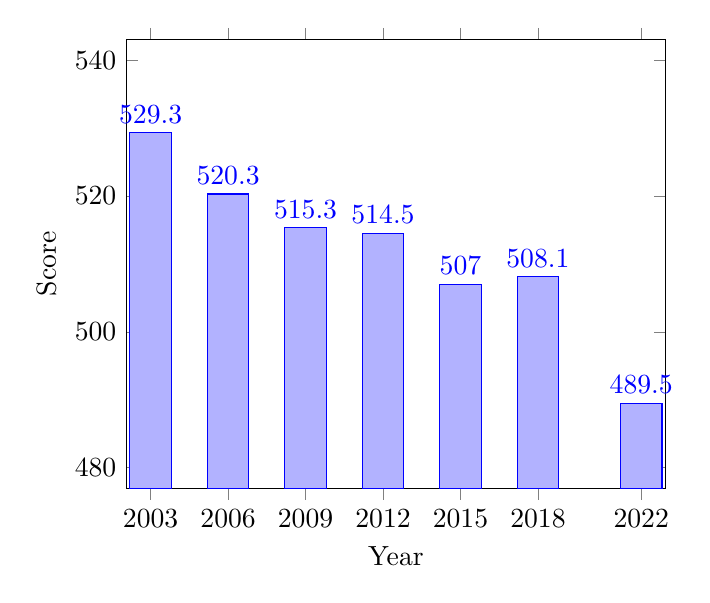
\begin{tikzpicture}
    \begin{axis}[
        xtick=data,
        x tick label style={
            /pgf/number format/1000 sep=},
        xlabel={Year},
        ylabel={Score},
        enlargelimits=0.05,
        ymin=480,
        ymax=540,
        ybar,
        bar width=15pt,
        nodes near coords,
        nodes near coords align={vertical},
    ]

    \addplot coordinates {
        (2003,529.3)
        (2006,520.3)
        (2009,515.3)
        (2012,514.5)
        (2015,507.0)
        (2018,508.1)
        (2022,489.5)
    };

    \end{axis}
    \end{tikzpicture}

    \caption{Evolution of Belgium's PISA mathematics scores from 2003 to 2022, showing a clear downward trend in average performance over time. \cite{globaleconomy2022belgium}}
    \label{fig:pisa_scores_belgium}
\end{figure}

What makes this field particularly active is that arithmetic turns out to be far more complex than it looks from the outside. On the surface, solving a sum seems straightforward. But decades of research have made clear that children bring a whole collection of cognitive skills to the table when they do arithmetic \cite{geary_chapter_2016}. These skills are still developing throughout primary school and that differ substantially from one child to the next. Some of these are specific to numbers: how well children process numerical quantities, or how quickly they retrieve arithmetic facts from memory \cite{vanbinst_chapter_2016}. Others are more general: how well they can hold information in mind \cite{zhang2022working}, how flexibly they switch between strategies \cite{hickendorff2022flexibility}, and perhaps most interestingly, how accurately they judge whether their own answers are correct \cite{rinne_knowing_2014}. De Smedt \cite{desmedt2022} provides an overview of this landscape, noting that individual differences in mathematical performance are remarkably stable and already visible before children enter formal education. Understanding which factors drive these differences, and how they interact across development, remains an open and active research question. 

Researchers at KU Leuven have been prominent contributors to this effort, particularly on the role of metacognitive monitoring in arithmetic achievement \cite{bellon_more_2019, bellon2020, bellon2021} and on individual differences in numerical magnitude processing \cite{vanbinst_chapter_2016}. These are not isolated efforts. Similar questions are being pursued by research groups internationally, each approaching the problem from a different angle \cite{geary_chapter_2016, ansari2025arithmetic, zhang2022working, hickendorff2022flexibility}.

All of this research depends on something practical: tools. Every study in this field depends on being able to observe children doing arithmetic under controlled conditions. Measuring not just whether they get the right answer, but how long it takes, how confident they are, and how their performance evolves over multiple sessions. The quality of that data depends directly on the quality of the tools used to collect it. As this thesis will argue, the tools currently available leave a significant gap between what researchers need and what is currently available. That gap is the starting point for this work.


\section{What a good research tool needs}
\label{sec:research-properties}
Before looking at what is currently available, it is worth being precise about what we are actually looking for. The previous section established that arithmetic research in primary school children is an active field with real scientific stakes. But good research questions can only produce good answers if the tools used to collect the data are up to the job. This section defines what that means in practice.

The six properties described below were developed through a combination of discussions with researchers in the field and a reading of how existing tools are evaluated in the literature on experimental software for educational psychology \cite{peirce_psychopypsychophysics_2007,mathot_opensesame_2012}. They are not claimed to be exhaustive, but together they capture the core requirements that a tool must meet if it is to support rigorous\footnote{In the context of this thesis, ``rigorous'' research is understood in the sense of Shadish, Cook, and Campbell \cite{shadish2002experimental}: research whose design, data collection, and analysis are controlled tightly enough to support valid causal inferences. In practice, this means controlling extraneous variables, collecting complete and accurate data, and producing results that generalise beyond the specific experimental session.}, classroom-based research with children. Each property is introduced and briefly motivated here. The question of how well existing tools satisfy them is taken up in the following section.

\paragraph{Data Tracking}
The most basic requirement of any research tool is that it records what happens. In arithmetic research this means logging not just whether a child answered correctly, but also the response time, the exact answer given, the confidence rating if applicable, and the precise timestamp of each event. Without clean, structured, and complete data, no analysis is possible. This sounds obvious, but in practice many tools either do not log enough detail, make the export process too complex, or produce formats that require preprocessing before they can be used. A good research tool must make data collection automatic, complete, and straightforward to access.

\paragraph{Experimental control}
Research designs in educational psychology typically involve comparing groups under different conditions. For example, children who receive metacognitive prompts versus those who do not. To draw valid conclusions from such a comparison, the researcher must be able to control precisely what each group sees and experiences. This includes controlling the type of exercises presented, the order in which they appear, which items are excluded, whether adaptive difficulty is active or not, and so on. Without this level of control, confounding variables (an outside, often hidden, third variable \cite{salkind2010encyclopedia}) creep in and the internal validity of the study (the extent to which observed effects are caused by the manipulation rather than to other factors \cite{campbell1963experimental}) is compromised.

\paragraph{Reproducibility}
A finding is only scientifically meaningful if it can be replicated. For a tool to support reproducible research, it must be possible to save the complete configuration of an experiment and share it with other researchers so they can run the exact same study. This is closely tied to broader discussions in the open science community about transparency and replication \cite{opensciencecollaboration2015}.

\paragraph{Flexibility}
A research tool is rarely used for a single study. Experiments differ from each other in countless ways, and the same tool needs to support all of them without having to be rebuilt from scratch.

In practice, this means that the parameters a researcher might want to vary need to live outside the source code. This goes beyond simple settings like the number of trials or the timing of how long an item is shown. It also includes structural choices: what kind of stimuli appear (sums, comparisons, word problems, images), how those stimuli are presented and in what order, which prompts the child sees, what counts as feedback, and how a session is organised. If these aspects are hard-coded, the tool does not just become inconvenient to adapt. It becomes impossible for a researcher (or a teacher building their own experiment) to set up the study they actually want. Hard-coded choices turn into real limitations on the study design, which is why flexibility has to be designed in from the start.

\paragraph{Reliability}
Reliability is the property that is easiest to take for granted and most damaging to lose. A research tool is reliable when it behaves the same way for every participant, every session, every time. Timings are accurate (precision), inputs are captured without loss, the interface does not stutter at unpredictable moments (stability), and a crash during session three of a four-session study does not destroy the data from sessions one and two (robustness). None of this is optional. The moment a tool becomes unreliable, the data it produces becomes hard to interpret: ``was that slow response time a real cognitive effect, or was the screen just slow to refresh that trial?'' The concern is not theoretical, millisecond-scale timing errors in commonly used experimental equipment have been documented as a reason for replication failures in reaction-time research \cite{plant2013millisecond}.

Reliability also means working everywhere the study is run, not just on the researcher's development machine. Classroom research typically spans multiple sessions over days or weeks, on hardware the researcher does not control: the school's laptops, the tablets in the library, a mix of browsers on a mix of operating systems. A tool that performs well only under ideal conditions is, for practical purposes, unreliable.

\paragraph{Ease of setup}
A tool can do everything described above perfectly and still be unusable if setting it up takes three weeks and a degree in computer science. The researchers who drive the field are, with few exceptions, not software engineers. If the tool they are meant to use assumes otherwise, there are really only two outcomes: either studies get delayed while someone else writes the experiment, or the study gets reshaped to fit what is easy to implement rather than what the research question actually requires.

Ease of setup is more than the absence of programming. It is the whole experience of getting from ``I want to run this study'' to ``the first child is doing the first exercise.'' Can the researcher tell, by looking at the interface, what each setting does? Is the navigation between configuration screens clear enough that a teacher could manage it during a short training session? When something is misconfigured, does the tool flag the problem before a classroom full of children is already logged in? Visual clarity and guidance through the setup process are what make the difference between a tool a researcher can use independently and one that requires constant developer support.

\section{Current research tools and their limitations}
\label{sec:research-tools}
With a clear picture of what a good research tool needs to do, the next step is to look at what researchers actually have on their desks today. This section walks through the two tools that came up most often during discussions with the research team at KU Leuven: OpenSesame \cite{mathot_opensesame_2012}, a tool frequently used by my co-supervisor in research projects (including the master's thesis discussed in Section \ref{sec:bellon-studies}), and PsychoPy \cite{peirce2019psychopy2}, which is taught to psychology students. The discussion examines how each of them fares against the six properties introduced in Section \ref{sec:research-properties}. Both tools have been carefully designed and have earned their place in the field. The point of this section is not to argue that they are bad tools; it is to show that even the best tools currently available leave a specific kind of gap, and that this gap becomes critical the moment a study leaves the controlled lab and moves into a classroom.

The discussion starts with OpenSesame, then turns to PsychoPy, and ends by drawing out the limitations that both tools share. That final discussion is what motivates the shift in direction taken in Chapter \ref{chp:exercise-tools}.

\subsection{OpenSesame}
Following its authors, OpenSesame is described as ``an open-source, graphical experiment builder for the social sciences'' \cite{mathot_opensesame_2012}. It was designed to make the construction of experiments in the social sciences more accessible than before by providing a graphical user interface (GUI) on top of a Python back-end. A researcher assembles an experiment by dragging items (trial loops, sketchpads, keyboard response components, inline scripts) into a tree structure that represents the flow of the study (as shown in Figure \ref{fig:opensesame_gui}). For anything the GUI does not cover, OpenSesame exposes an inline Python editor that lets the researcher drop directly into code \cite{mathot_opensesame_2012}. It is cross-platform and free.

Against the six properties from Section \ref{sec:research-properties}, OpenSesame scores well on most of them. \textbf{Data tracking} is handled automatically: every trial produces a row in a structured log file, with response times, accuracy, and any custom variables the experimenter defines. \textbf{Experimental control} is one of its strongest points. The researcher has essentially full authority over what each participant sees, the order of stimuli, the exact timing of each event, and the conditions under which the experiment branches. \textbf{Reproducibility} is built into the format: an OpenSesame experiment is stored as a single file that bundles the configuration, the stimuli, and any inline scripts, which means that sharing the experiment with a collaborator is as simple as sharing that file. \textbf{Flexibility} is high because the inline Python escape hatch means there is almost no experimental design the tool cannot, in principle, express. \textbf{Reliability} is more nuanced. Timing precision was measured in an independent benchmark using a hardware Black Box Toolkit, where OpenSesame fell within a 1--5 ms range across visual, audio, and response measures, and performed consistently across Windows, macOS, and Ubuntu \cite{bridges2020timing}. The broader, practical sense of reliability is harder to pin down. Because OpenSesame is a separate software package that has to be installed and configured correctly on each machine, we have heard of cases where it is awkward to get running on classroom hardware. Overall, though, the tool can be considered reliable.

The property where OpenSesame runs into trouble is \textbf{ease of setup}. On the surface, the GUI looks approachable: drag some items, connect them, press run. But the moment the study steps outside the standard kind of experiment where a stimulus is shown and the participant gives a response, the researcher is pulled into Python. Adding a custom adaptive algorithm, implementing a non-trivial exclusion rule, conditionally showing feedback based on the previous answer, or linking trial sequences across multiple sessions: each of these require inline scripts. These scripts are not decoration, they become critical components of the experiment, and maintaining them demands real programming skill. A researcher without a background in Python is effectively stuck with what the GUI alone can do, which for any non-standard arithmetic study is not enough.

\begin{figure}
  \centering
  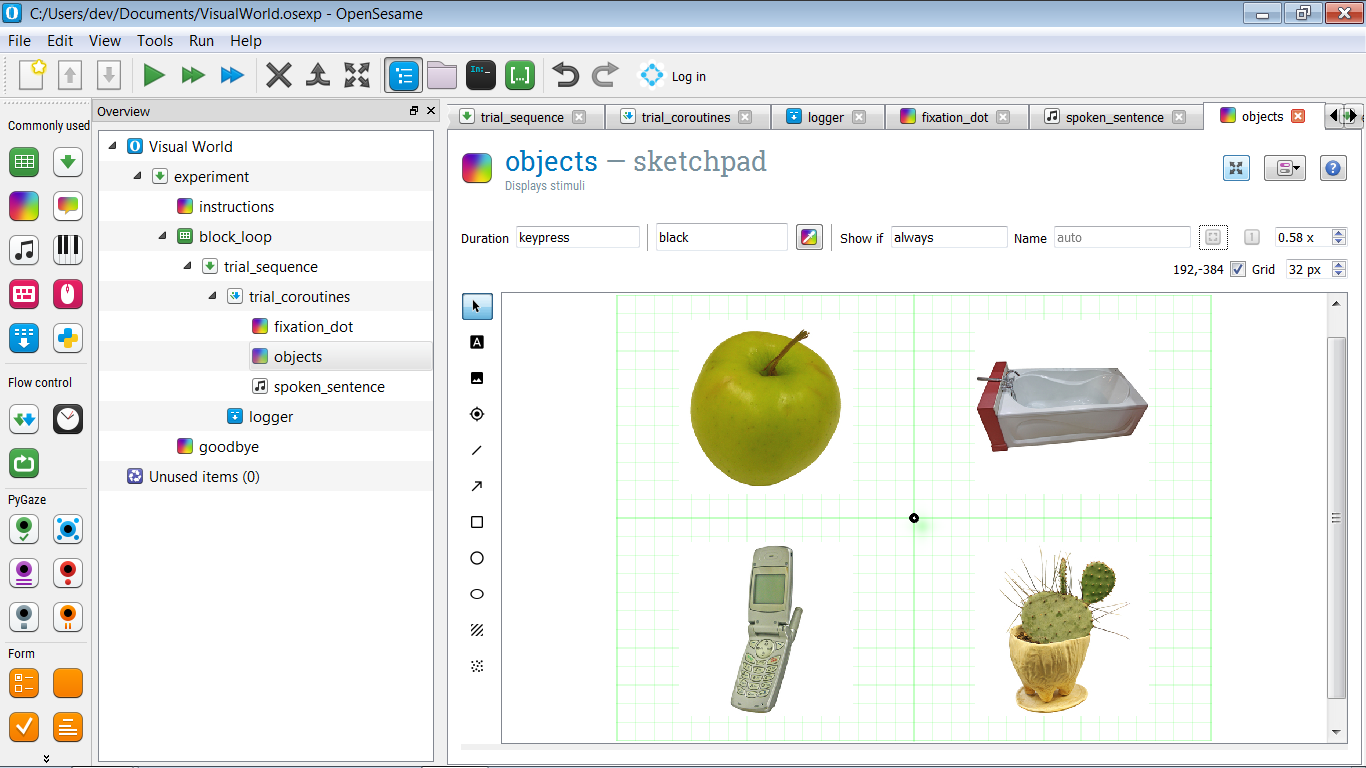
\includegraphics[width=0.85\textwidth]{figures/opensesame_gui.png}
  \caption{Screenshot of the OpenSesame graphical user interface, showing the experiment structure on the left and a sketchpad editor for designing visual stimuli on the right.
  {\cite{mathot_opensesame_2012}}}
  \label{fig:opensesame_gui}
\end{figure}

There is also a second layer to this problem that has little to do with programming. OpenSesame exposes a large number of configuration options across several panels and tabs, with defaults and vocabulary (loops, sketchpads, synchronisation back-ends) that only make sense once the underlying experiment-building model is already familiar. For an experienced user this is manageable, but for someone approaching the tool for the first time the learning curve is steep enough that they will typically need a trained research assistant in the room.

The OpenSesame team continues to develop the project (including a new generative-AI setup assistant \cite{sigmundai} and a web version \cite{mathot2022osweb}), but the underlying picture is unchanged: anything beyond the standard GUI workflow still requires Python. OpenSesame is a powerful tool, but for researchers without a programming background it is limiting.

\subsection{PsychoPy}
PsychoPy is the other open-source tool that comes up frequently in this work. Originally developed by Peirce as a Python library for psychophysics experiments \cite{peirce_psychopypsychophysics_2007}, it has since grown into a full experiment-building environment with its own graphical Builder interface \cite{peirce2019psychopy2}. Where OpenSesame started from the GUI and added Python as an escape hatch, PsychoPy came from the opposite direction: it began as a pure coding library and later wrapped a graphical interface around it. This difference in origin matters because it affects how the tool behaves from a user's perspective.

On the first five properties, PsychoPy performs comparably to OpenSesame. \textbf{Data tracking}, \textbf{experimental control}, \textbf{reproducibility}, and \textbf{flexibility} are all handled at a similar level: logging is automatic and extensible, the researcher has full control over what each participant sees, experiments can be saved and shared as structured files, and the underlying Python library means almost any design can be expressed in code. \textbf{Reliability} is where PsychoPy stands out the most. It was originally developed because existing tools did not offer the timing accuracy that psychophysics research demands \cite{peirce_psychopypsychophysics_2007}, and independent benchmarks confirm that it remains among the most precise lab-based tools available, with mean visual, audio, and response timing under one millisecond \cite{bridges2020timing}. It is also a mature project with a large active community of users and developers \cite{peirce2019psychopy2}, which means bugs tend to be identified and fixed quickly. Like OpenSesame, however, it was designed for controlled lab environments rather than for the hardware mix of a primary school classroom.

That leaves \textbf{ease of setup}, where PsychoPy faces the same fundamental challenge as OpenSesame, but arguably in a more obvious form. The graphical Builder interface offers a drag-and-drop workflow that works well for simple experiments. PsychoPy's own documentation is explicit about the trade-off: the Builder covers standard cases, and for anything more complex the researcher is expected to write raw Python code \cite{peirce2019psychopy2}.

The interface itself reinforces this. A first-time user is confronted with terminology like Routines, Components, Backends, and Monitor configurations: concepts that make sense to someone with a programming background but are not self-evident to a researcher encountering the tool for the first time. The Builder GUI is genuinely well-designed and capable (Figure~\ref{fig:psychopy-ui}), but where OpenSesame attempts to hide the Python layer behind a familiar drag-and-drop tree, PsychoPy keeps it closer to the surface. The result is similar to OpenSesame but shifted further along the technical axis: an excellent tool for a researcher who already knows Python or is willing to learn it, but a steep entry point for anyone else.

\begin{figure}
\centering
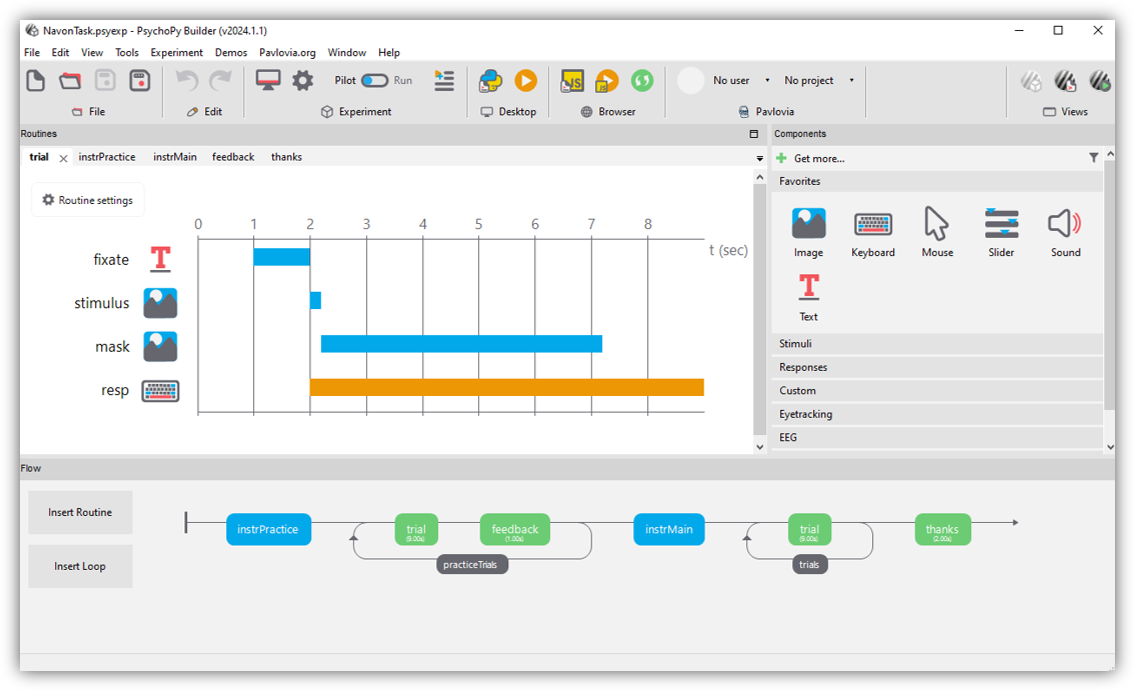
\includegraphics[width=0.85\textwidth]{figures/psychopy_builder.png}
\caption{The PsychoPy Builder interface. Routines are displayed as timelines, and each Component maps onto a set of Python parameters. For experiments that exceed the Builder's built-in Components, researchers insert Code Components containing raw Python, which effectively turns the study into a programming project.}
\label{fig:psychopy-ui}
\end{figure}

At this point, a pattern is becoming visible. Both OpenSesame and PsychoPy satisfy the core research requirements but both run into the same wall when it comes to ease of setup. Figure~\ref{fig:research-tool-grid} summarises this comparison. The six research-tool properties from Section \ref{sec:research-properties} are listed as columns, and each tool is evaluated per property. The first five columns are green; the last one is not. This grid will be extended in Chapter \ref{chp:exercise-tools} when the exercise-tool properties are introduced.

\begin{figure}
\centering
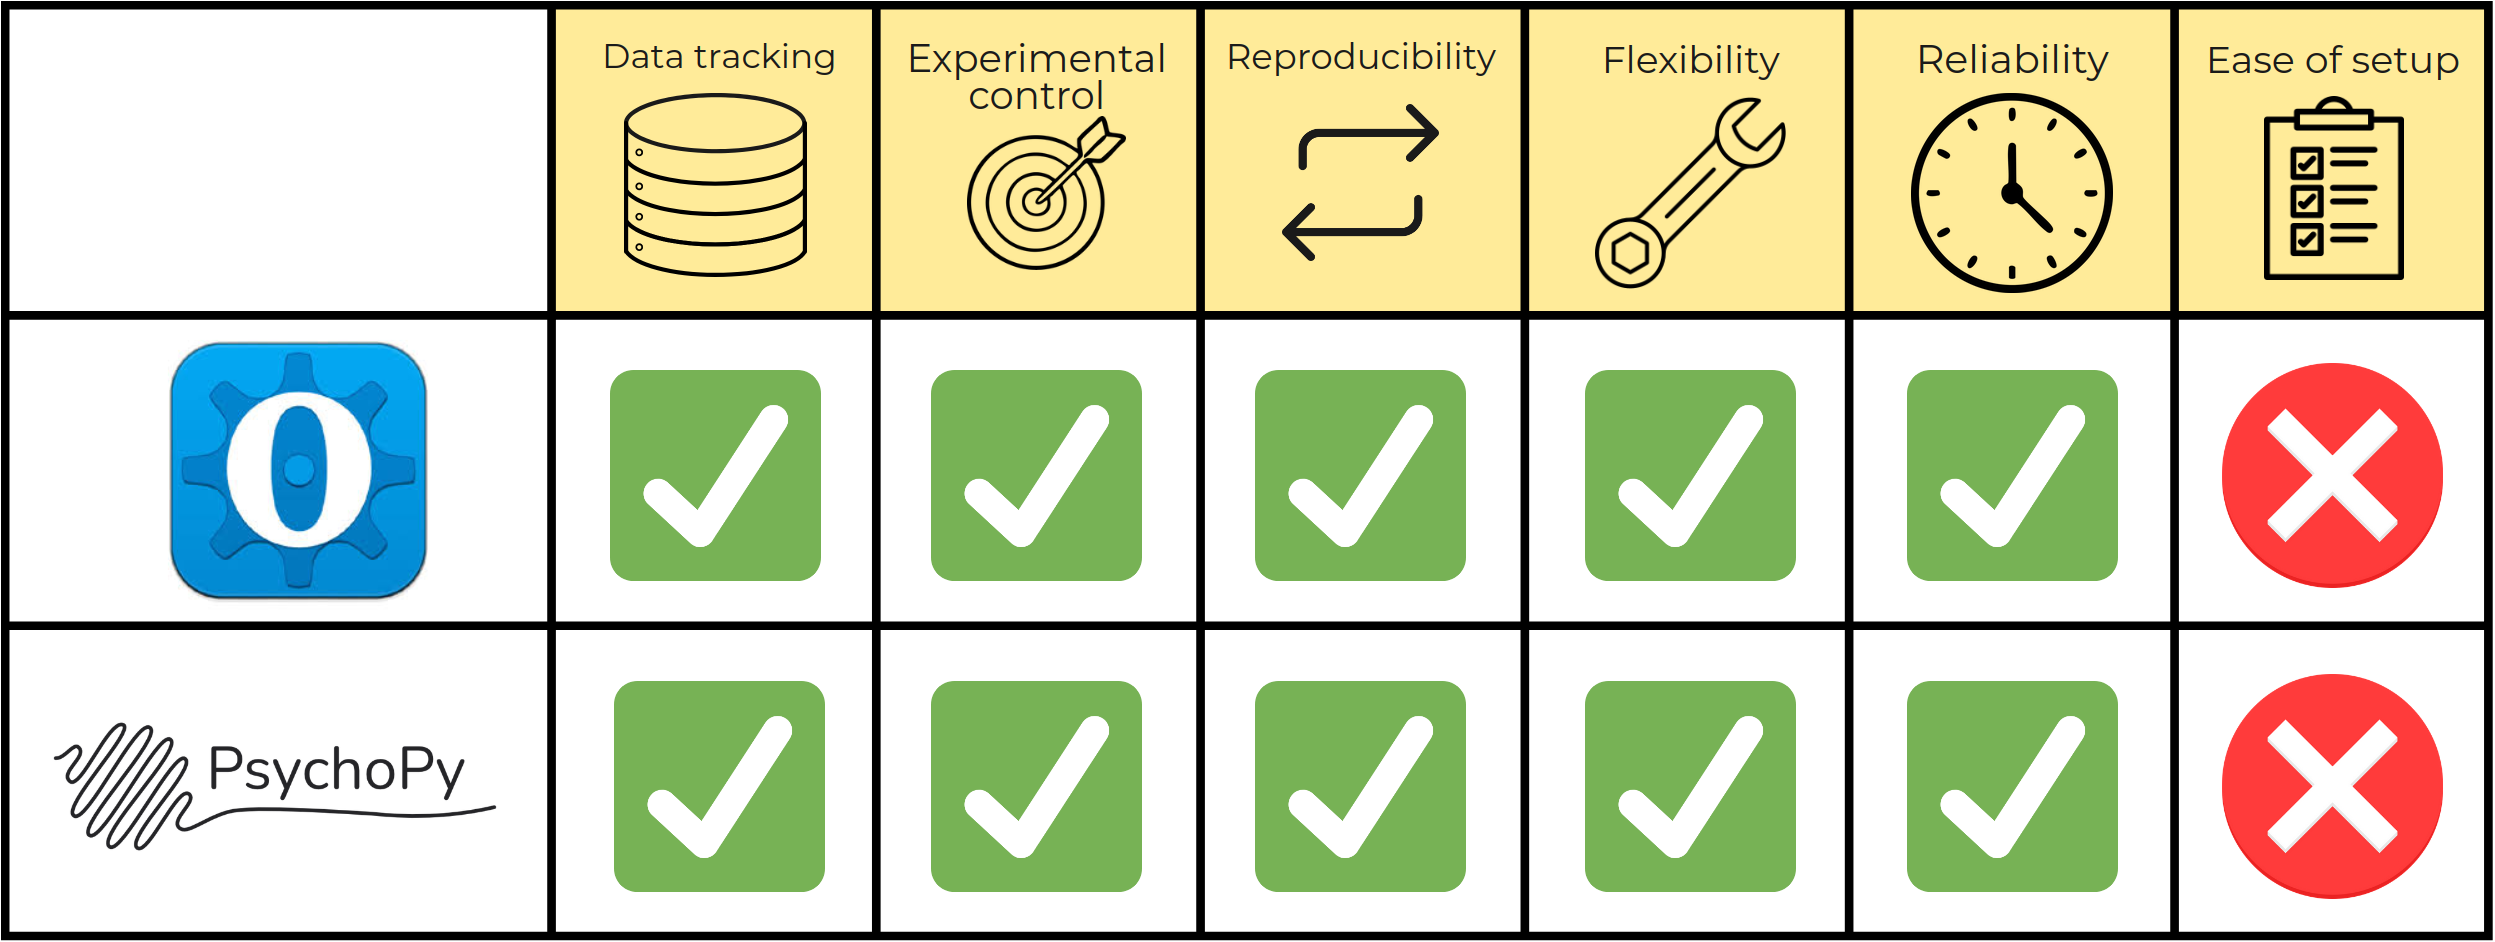
\includegraphics[width=0.85\textwidth]{figures/grid_research_new.png}
\caption{Comparison of OpenSesame and PsychoPy against the six research-tool properties from Section \ref{sec:research-properties}. Both tools satisfy all but the last.}
\label{fig:research-tool-grid}
\end{figure}

\subsection{Shared limitations}
\label{sec:shared-limitations}
The previous sections have shown that OpenSesame and PsychoPy are strong research tools. On five of the six properties defined in Section \ref{sec:research-properties} they deliver exactly what a researcher needs: clean data tracking, full experimental control, reproducible setups, flexible designs, and reliability. But the picture changes completely when you step back and ask a different question: what is it actually like for a child to sit in front of one of these tools?

The answer, in most cases, is that it is not a pleasant experience. A typical arithmetic experiment built in OpenSesame or PsychoPy presents the child with white text on a black screen, one problem at a time, with no story, no colour, no reward, and no sense of progress (see example Figure \ref{fig:black_screen}). There is no character guiding them through the session or puzzle to unlock after ten correct answers. The experiment simply moves from one trial to the next until it is done. For a single short session in a quiet lab, this can work. But arithmetic research often takes place in classrooms, across multiple sessions spread over days or weeks, with children who are seven or eight years old. In that context, a black screen with numbers on it is not enough.

This is not an oversight by the developers of these tools. OpenSesame and PsychoPy were built to be general-purpose experiment builders, and they do that job well. The problem is the one identified in the previous sections: anything beyond the bare stimulus-response loop, gamification, a narrative wrapper, a child-friendly login, has to be built from scratch by the researcher, in Python. Because of the ease-of-setup wall, the researchers who need these features cannot build them. They know exactly what kind of experience they want the child to have, exercises that adapt to the child's level, a colourful interface that feels like a game, metacognitive prompts wrapped in a story. But translating that vision into working code is a skill most of them do not have, and hiring or collaborating with a developer for every study is neither practical nor scalable.

\begin{figure}
\centering
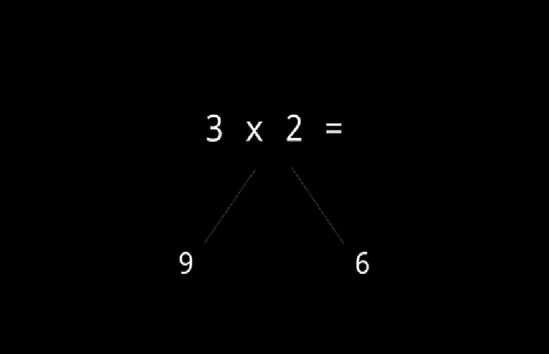
\includegraphics[width=0.65\textwidth]{figures/zwart_scherm.png}
\caption{Example of a stimulus presentation screen created in OpenSesame, showing a simple arithmetic task with multiple-choice response options.}
\label{fig:black_screen}
\end{figure}

This creates a frustrating situation. Researchers who study arithmetic learning in children know their population well. They know what kind of experience would actually serve the child sitting in front of the screen, and how that experience would in turn serve the data they collect. Yet the tools at their disposal make any of that difficult to deliver without significant programming effort. The result is a forced compromise: researchers know what they want, often something that resembles the classroom environment the research is trying to understand, but they cannot deliver it. They end up running studies in conditions stripped of the context they actually care about.

Whether this matters, and how much it matters, is the question taken up in the next section.

\section{Why this matters: the cost of a bad research tool}
\label{sec:why-this-matters}
The limitations described in Section \ref{sec:research-tools} are not just inconveniences for the researcher setting up a study. They have direct consequences for the quality of the research itself. When the tool a child interacts with during an experiment is unfamiliar, visually unappealing, and lacking in motivational features, the data that comes out of that experiment is affected in ways that are hard to control for after the fact. This section discusses three mechanisms through which a poor research tool can compromise a study: reduced ecological validity, motivation drop across sessions, and confounding caused by tool unfamiliarity.

\subsection{Ecological validity}

Ecological validity refers to how well the conditions of a study match the real-world context the research aims to understand \cite{bronfenbrenner1977toward}. Bronfenbrenner argued that studies conducted in artificial laboratory settings, which differ from children's everyday environments, often produce results that are difficult to generalise. Instead, he emphasised the importance of conducting research in natural settings where learning actually occurs, even if these settings are more complex \cite{bronfenbrenner1977toward}.

Shadish, Cook, and Campbell make a similar point in the context of experimental design more broadly: highly controlled lab environments improve internal validity but at the cost of external validity, because the conditions no longer reflect the dynamic nature of real-world learning \cite{shadish2002experimental}.

For arithmetic research with primary school children, this trade-off becomes very concrete. Children today learn arithmetic in environments that adapt to their level, use game-like elements, and let them exercise some control over what they do next. Adaptive difficulty, exercises that get easier or harder based on how the child is doing, keeps learners in a zone where the task is challenging enough to require effort but not so hard that they give up (i.e., zone of proximal development [ZPD]) \cite{murray_zpd_2006}. Adaptive arithmetic learning apps have been shown to improve learning gains and engagement in kindergarten and early primary-school children \cite{bang2023mymathacademy}. Recent systematic reviews have shown that gamification can positively impact the academic performance, motivation, and engagement of primary school children \cite{manzanoleon2021gamification}. A research tool that strips all of these features away does not just produce a less pleasant experience for the child, it produces an experience that no longer resembles the classroom context the research is ultimately trying to study. Whatever is measured under those conditions is, by Bronfenbrenner's definition, less ecologically valid.

\subsection{Motivation drop}
The second cost is more practical and arguably more damaging: children lose motivation. Arithmetic research often spans multiple sessions across days or weeks, and this only works if children stay engaged throughout. Performance on cognitively demanding tasks declines as a function of time on task, and short breaks or changes in activity can partially restore it \cite{sievertsen2016cognitive}. That finding is about fatigue within a single day, but it points to the same underlying issue at the multi-session scale: sustained mental effort produces measurable performance costs, and those costs accumulate when nothing in the task itself works against them.

When the tool itself offers no variation, no rewards, no story, and no sense of progress, the motivation problem is amplified. Research on the role of motivation in mental fatigue has shown that participants who receive motivational incentives are able to maintain performance levels on demanding tasks over extended periods, while those in non-rewarded conditions show clear performance declines \cite{hopstaken2015role}. In the context of arithmetic research with children, this translates to a concrete risk: if the experiment feels boring by session two, the data from sessions three and four may reflect disengagement rather than actual arithmetic ability. The researcher ends up measuring motivation, not mathematics.

The features that could prevent this, gamification, narrative framing, and immediate feedback, are known to support engagement and motivation over time \cite{manzanoleon2021gamification}. They are also precisely the features that most research experiments lack and that the programming barrier described in Section \ref{sec:research-tools} makes difficult to add.

\subsection{The familiarity effect}
The third mechanism is subtler but no less important. When a child encounters a completely unfamiliar tool during a research session, the tool itself becomes a variable in the experiment. The child has to figure out where to type an answer, what the buttons do, how the feedback works, and what is expected of them, all while supposedly demonstrating their arithmetic ability. A related effect is well documented in the testing literature: children tested by a familiar examiner score about 0.28 standard deviations higher than those tested by an unfamiliar one \cite{fuchs1986test}. The same logic plausibly applies to the tool itself: unfamiliarity is a source of irrelevant cognitive load that lowers performance.

If the research tool were also used outside of the experiment, for regular classroom practice or homework, the tool would be invisible during the study in the way a pencil is invisible during a written test: present, but not a source of confusion. The data would more cleanly reflect what the study is actually trying to measure. There is a second advantage too: discoveries made through research, for example that metacognitive prompts improve arithmetic learning, could be fed back into the same tool and reach children as part of their regular practice. The tool would not only serve research but also benefit from it.

\subsection{The bottom line}
All three mechanisms point in the same direction. A research tool that is ecologically valid, motivationally engaging, and familiar to the children who use it is not a luxury or a nice-to-have. It is a prerequisite for producing data that accurately reflects what it claims to measure. In short: a better tool means better research. The question, then, is where to find such a tool. The natural place to look is at the platforms children already use for arithmetic practice in classrooms. That is the direction taken in Chapter \ref{chp:exercise-tools}.

\section{A concrete example}
\label{sec:bellon-studies}
 
The previous section argued, on theoretical and general empirical grounds, that a research tool offering little variation, reward, or sense of progress amplifies the motivation problem across multiple sessions. It is worth grounding that argument in a concrete case. This section looks at one recent master's thesis that ran a multi-session arithmetic training in OpenSesame, the kind of bare stimulus-response setup described in Section~\ref{sec:shared-limitations}. The data from that study are limited, and the patterns described below are at the level of eyeballing rather than formal statistical testing. Still, they offer a concrete illustration of the motivation drop predicted in the previous section.\footnote{The study discussed here is an unpublished master's thesis \cite{baeten2025}. Its results have not undergone peer review, and the patterns reported below should therefore be interpreted with appropriate caution. They are used here as an illustration of a mechanism, not as a definitive empirical claim.}
 
Baeten \cite{baeten2025} studied the relationship between metacognitive monitoring and the arithmetic learning process in 161 third-grade children. To produce a learning process, the children completed a four-day arithmetic training built in OpenSesame, solving the same set of two-digit multiplication exercises once per day across four consecutive school days. Each daily session consisted of 64 items, presented as white text on a black screen with feedback after every answer. This is exactly the type of multi-session, low-engagement experiment that Section~\ref{sec:why-this-matters} identified as being at risk of measuring motivation rather than mathematics.
 
The thesis itself notes this risk. In its discussion of limitations, the author observes that having children complete the same task on four consecutive days can reduce task interest, and that accuracy appeared to stagnate after the second training day rather than continuing to improve \cite{baeten2025}. The thesis also already proposes a partial solution: it suggests that follow-up research could use rewards that depend on the participants' performance, so that children are sufficiently reinforced \cite{baeten2025}. To examine the within-day pattern more closely, the data from the second training day were analysed session by session. Each training day was divided into four successive sessions of sixteen items, and average response time and average accuracy were computed for each session. The result is shown in Figure~\ref{fig:motivation-drop-day2}.
 
\begin{figure}
    \centering
    \begin{subfigure}[t]{0.49\textwidth}
        \centering
        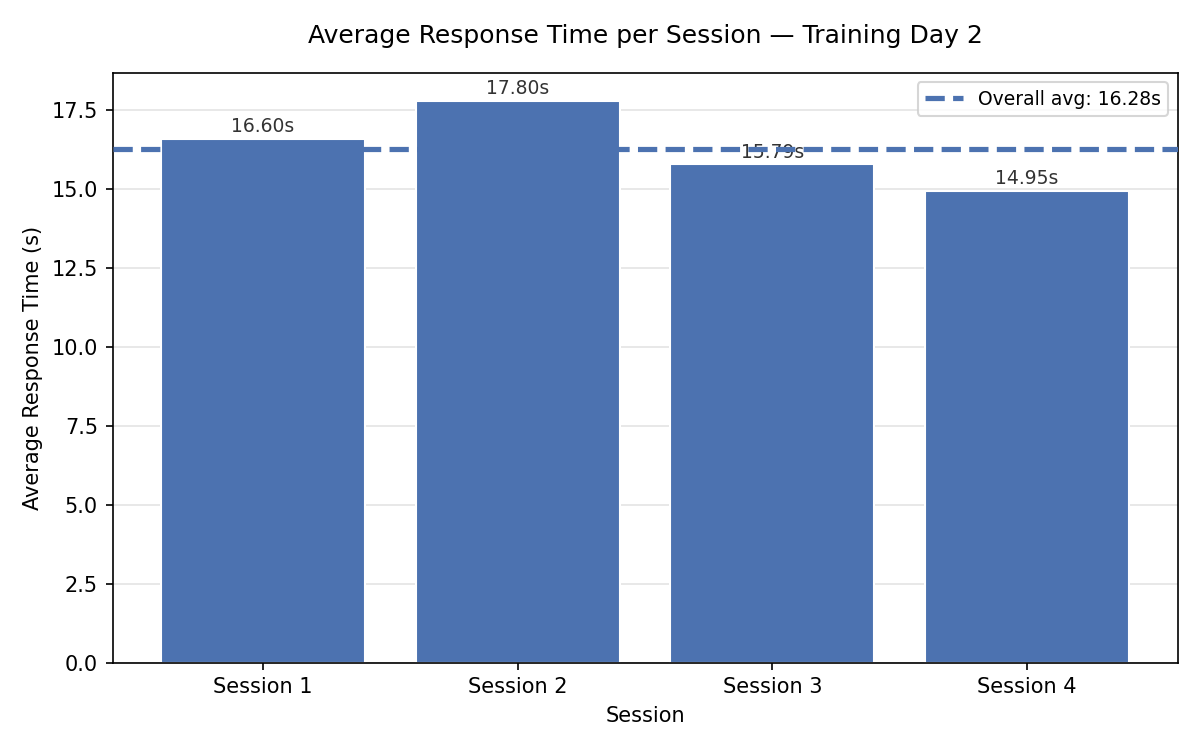
\includegraphics[width=\textwidth]{figures/rt_by_session_day2.png}
        \caption{Average response time per session.}
        \label{fig:rt-day2}
    \end{subfigure}
    \hfill
    \begin{subfigure}[t]{0.49\textwidth}
        \centering
        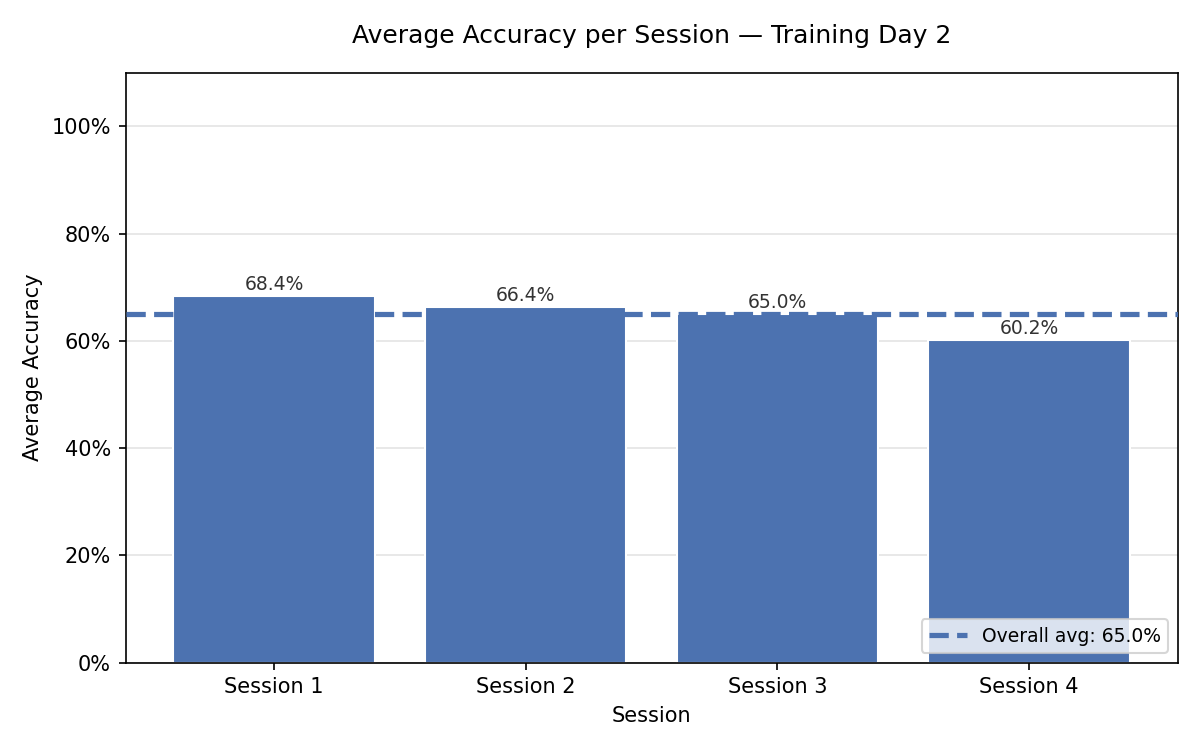
\includegraphics[width=\textwidth]{figures/accuracy_by_session_day2.png}
        \caption{Average accuracy per session.}
        \label{fig:accuracy-day2}
    \end{subfigure}
    \caption{Within-day change across the four sessions of training day~2 in the arithmetic training of Baeten \cite{baeten2025}. As the day progresses, children answer faster while becoming less accurate.}
    \label{fig:motivation-drop-day2}
\end{figure}
 
The two panels point in the same direction. After a small initial rise, the children's average response time falls steadily over the day, from 17.80 seconds in the second session down to 14.95 seconds in the fourth. If this were the only trend, it could be read as a sign of practice or growing fluency. But it is accompanied by the opposite movement in accuracy: the proportion of correct answers drops from 68.4\% in the first session to 60.2\% in the fourth. Children are not getting faster because they are getting better; they are getting faster while getting worse. That combination, shorter response times together with falling accuracy, is consistent with children rushing through the task: clicking quickly to reach the end rather than working through each problem. It appears to be the within-day counterpart of the motivation drop discussed in Section~\ref{sec:why-this-matters}, and it shows up already on the second of four training days.
 
This reading fits what experienced arithmetic researchers report seeing in practice. Bellon (personal communication, 2025) describes three converging signals of waning engagement in this kind of multi-session study. The first is observational: testers notice changes in children's attitude and involvement, such as less task-focused behaviour and less sustained effort. The second is in the behavioural data itself, where disengagement leaves traces such as sudden drops in accuracy, exercises skipped by clicking through quickly, very short response times, and sometimes nonsense answers. The third concerns the learning trajectories: where one would ideally expect gradual progress across training days, that progress is often absent or only weak. The faster-but-less-accurate pattern in Figure~\ref{fig:motivation-drop-day2} is broadly in line with these signals.
 
The lesson here is not that the study was poorly designed. The training was carefully constructed and ran on a capable, widely used research platform, and the thesis itself anticipated the motivation problem and proposed a reward-based fix. The point is rather that delivering such a fix is left entirely to the researcher. A research tool that provided engagement and performance-based rewards by default would lower that barrier, so that addressing the motivation drop does not depend on the individual researcher's programming effort.
 


% !TeX root = ../thesis.tex
\chapter{Exercise Tools}
\label{chp:exercise-tools}
The previous chapter established that the tools currently used for arithmetic research do their job as research instruments but fail as experiences for the children who use them. They lack the motivational, adaptive, and visual qualities that keep children engaged across multiple sessions, and the programming barrier makes it impractical for researchers to add these qualities themselves. The question that follows naturally is: where do these qualities already exist?

The answer is not far away. Across primary schools in Belgium and the Netherlands, children already use digital tools for arithmetic practice on a daily basis. Platforms like Automatus \cite{automatus} and Rekentuin \cite{rekentuin} are designed from the ground up to be engaging, adaptive, and easy for children to use. They look like games, they feel like games, and children are willing to spend time on them without being asked twice. In other words, these tools already solve many of the problems identified in Section \ref{sec:why-this-matters}: they offer the ecological validity, the sustained motivation, and the familiarity that research experiments lack.

This chapter examines exercise tools as a possible solution direction. It begins by defining what makes a good exercise tool, then walks through two prominent examples in the field, and ends by asking the inevitable follow-up question: if exercise tools solve the engagement problem, can they also serve as research tools? The answer, as will become clear, is not quite.

\section{What a good exercise tool needs}
\label{sec:exercise-properties}
Where Section \ref{sec:research-properties} asked what a research tool needs, this section asks the same question for the other side: what makes a good tool for arithmetic practice in the classroom? The properties listed below were developed through discussions with primary school teachers, educational researchers, and the co-supervisor of this thesis. They are not claimed to be exhaustive, but together they capture what practitioners in the field consistently identify as important. Where possible, connections to the educational psychology literature are drawn to ground these observations in theory.

\paragraph{Adaptivity}
Perhaps the single most important property of a good exercise tool is that it adapts to the child using it. Not every child in a classroom is at the same level, and a tool that presents the same exercises to everyone will inevitably bore the strongest students and frustrate the weakest ones. 

This idea has deep theoretical roots: Vygotsky's zone of proximal development (ZPD) is the gap between what a child can do on their own and what they can do with a little help \cite{vygotsky1978mind}. Csikszentmihalyi's flow theory makes a closely related point about engagement more generally, namely that people concentrate best when the difficulty of a task is well-matched to their skill level \cite{csikszentmihalyi1990flow}. In the specific case of arithmetic learning apps for young children, this is more than theory: Bang, Li, and Flynn showed that an adaptive arithmetic app produced significantly larger learning gains and stronger engagement than a non-adaptive control \cite{bang2023mymathacademy}. An exercise tool that does not adapt is, in effect, guaranteeing that most of the children using it will be working below or above their level most of the time.

\paragraph{Engagement}
Adaptivity keeps the difficulty right, but it does not on its own make a child want to open the tool again tomorrow. Engagement is about everything else that makes the experience feel worthwhile: a story that gives context to the exercises, visual rewards for progress, puzzles to unlock, a character to interact with. These are gamification elements, and systematic reviews of gamification in education consistently find that elements such as points, levels, narrative framing, and immediate feedback improve motivation and engagement in mathematics \cite{manzanoleon2021gamification}. For an exercise tool aimed at primary school children, engagement is not optional. A tool that children do not want to use is a tool that does not get used, regardless of how well-designed its exercises are.

\paragraph{Feedback}
Children need to know whether they got the answer right, and ideally they need to know it immediately. Delayed or absent feedback leaves the child uncertain about whether they are learning, and it removes one of the most natural drivers of improvement: the desire to correct a mistake you just made. Meta-analyses of educational feedback confirm that corrective, computer-delivered feedback is among the most effective forms, particularly for new skills \cite{wisniewski2020power}. Interestingly, more is not always better: in a recent study with elementary children, feedback that simply showed the correct answer led to greater persistence and more flexible strategy use than feedback that also added an explicit ``right/wrong'' verification cue \cite{merrick2024feedback}. The key is that feedback is timely, clear, and meaningful.

\paragraph{Personalisation}
Personalisation gives the child the feeling that the tool is theirs. This has two sides. The first is functional: letting children choose which type of exercise to practise, whether they want to see a timer, or what difficulty level they prefer. This kind of choice can give children a sense of ownership: a child who decides to practise multiplication because they know it is their weakest area is doing something more valuable than just answering another question. The second side is personal identity: an avatar, a nickname, a progress tracker that shows their journey, a customised home screen. These elements may seem cosmetic, but they transform a generic program into something that feels like it belongs to the child, which in turn makes the child more likely to come back to it \cite{cordova1996intrinsic}.

\paragraph{Accessibility}
An exercise tool is only useful if children can actually reach it. In practice this means the tool should run in a web browser, work on the devices that schools actually have (laptops, tablets, Chromebooks), and not require any software installation. It also means the tool should be available outside the classroom, so that children can practise at home if they want to. 

\paragraph{User friendliness}
Finally, the tool has to be usable by its target audience, which in this case is children between roughly seven and eleven years old. This means large buttons, clear icons, simple navigation, and a visual language that children understand without needing instructions. Every unnecessary interface element adds extraneous cognitive load, the kind of mental effort that does not contribute to learning, and so takes working memory away from the actual exercise \cite{mayer2003nine}. 

\section{Existing exercise tools: Automatus and Rekentuin}
\label{sec:exercise-tools}

\subsection{Automatus}
Automatus \cite{automatus} is a web-based arithmetic practice platform used in primary schools across Flanders and the Netherlands. It was designed with a clear purpose: to help children automate their arithmetic skills through repeated, structured practice. Teachers assemble customised ``lands'' consisting out of tiles, where each tile corresponds to a specific type of problem (for example, additions up to 20, or the multiplication table of 7). Children then work their way through these tiles, with the map giving each session a visible sense of direction and progression. Figure~\ref{fig:automatus_ui} shows the tile screen children encounter while practising.

\begin{figure}
\centering
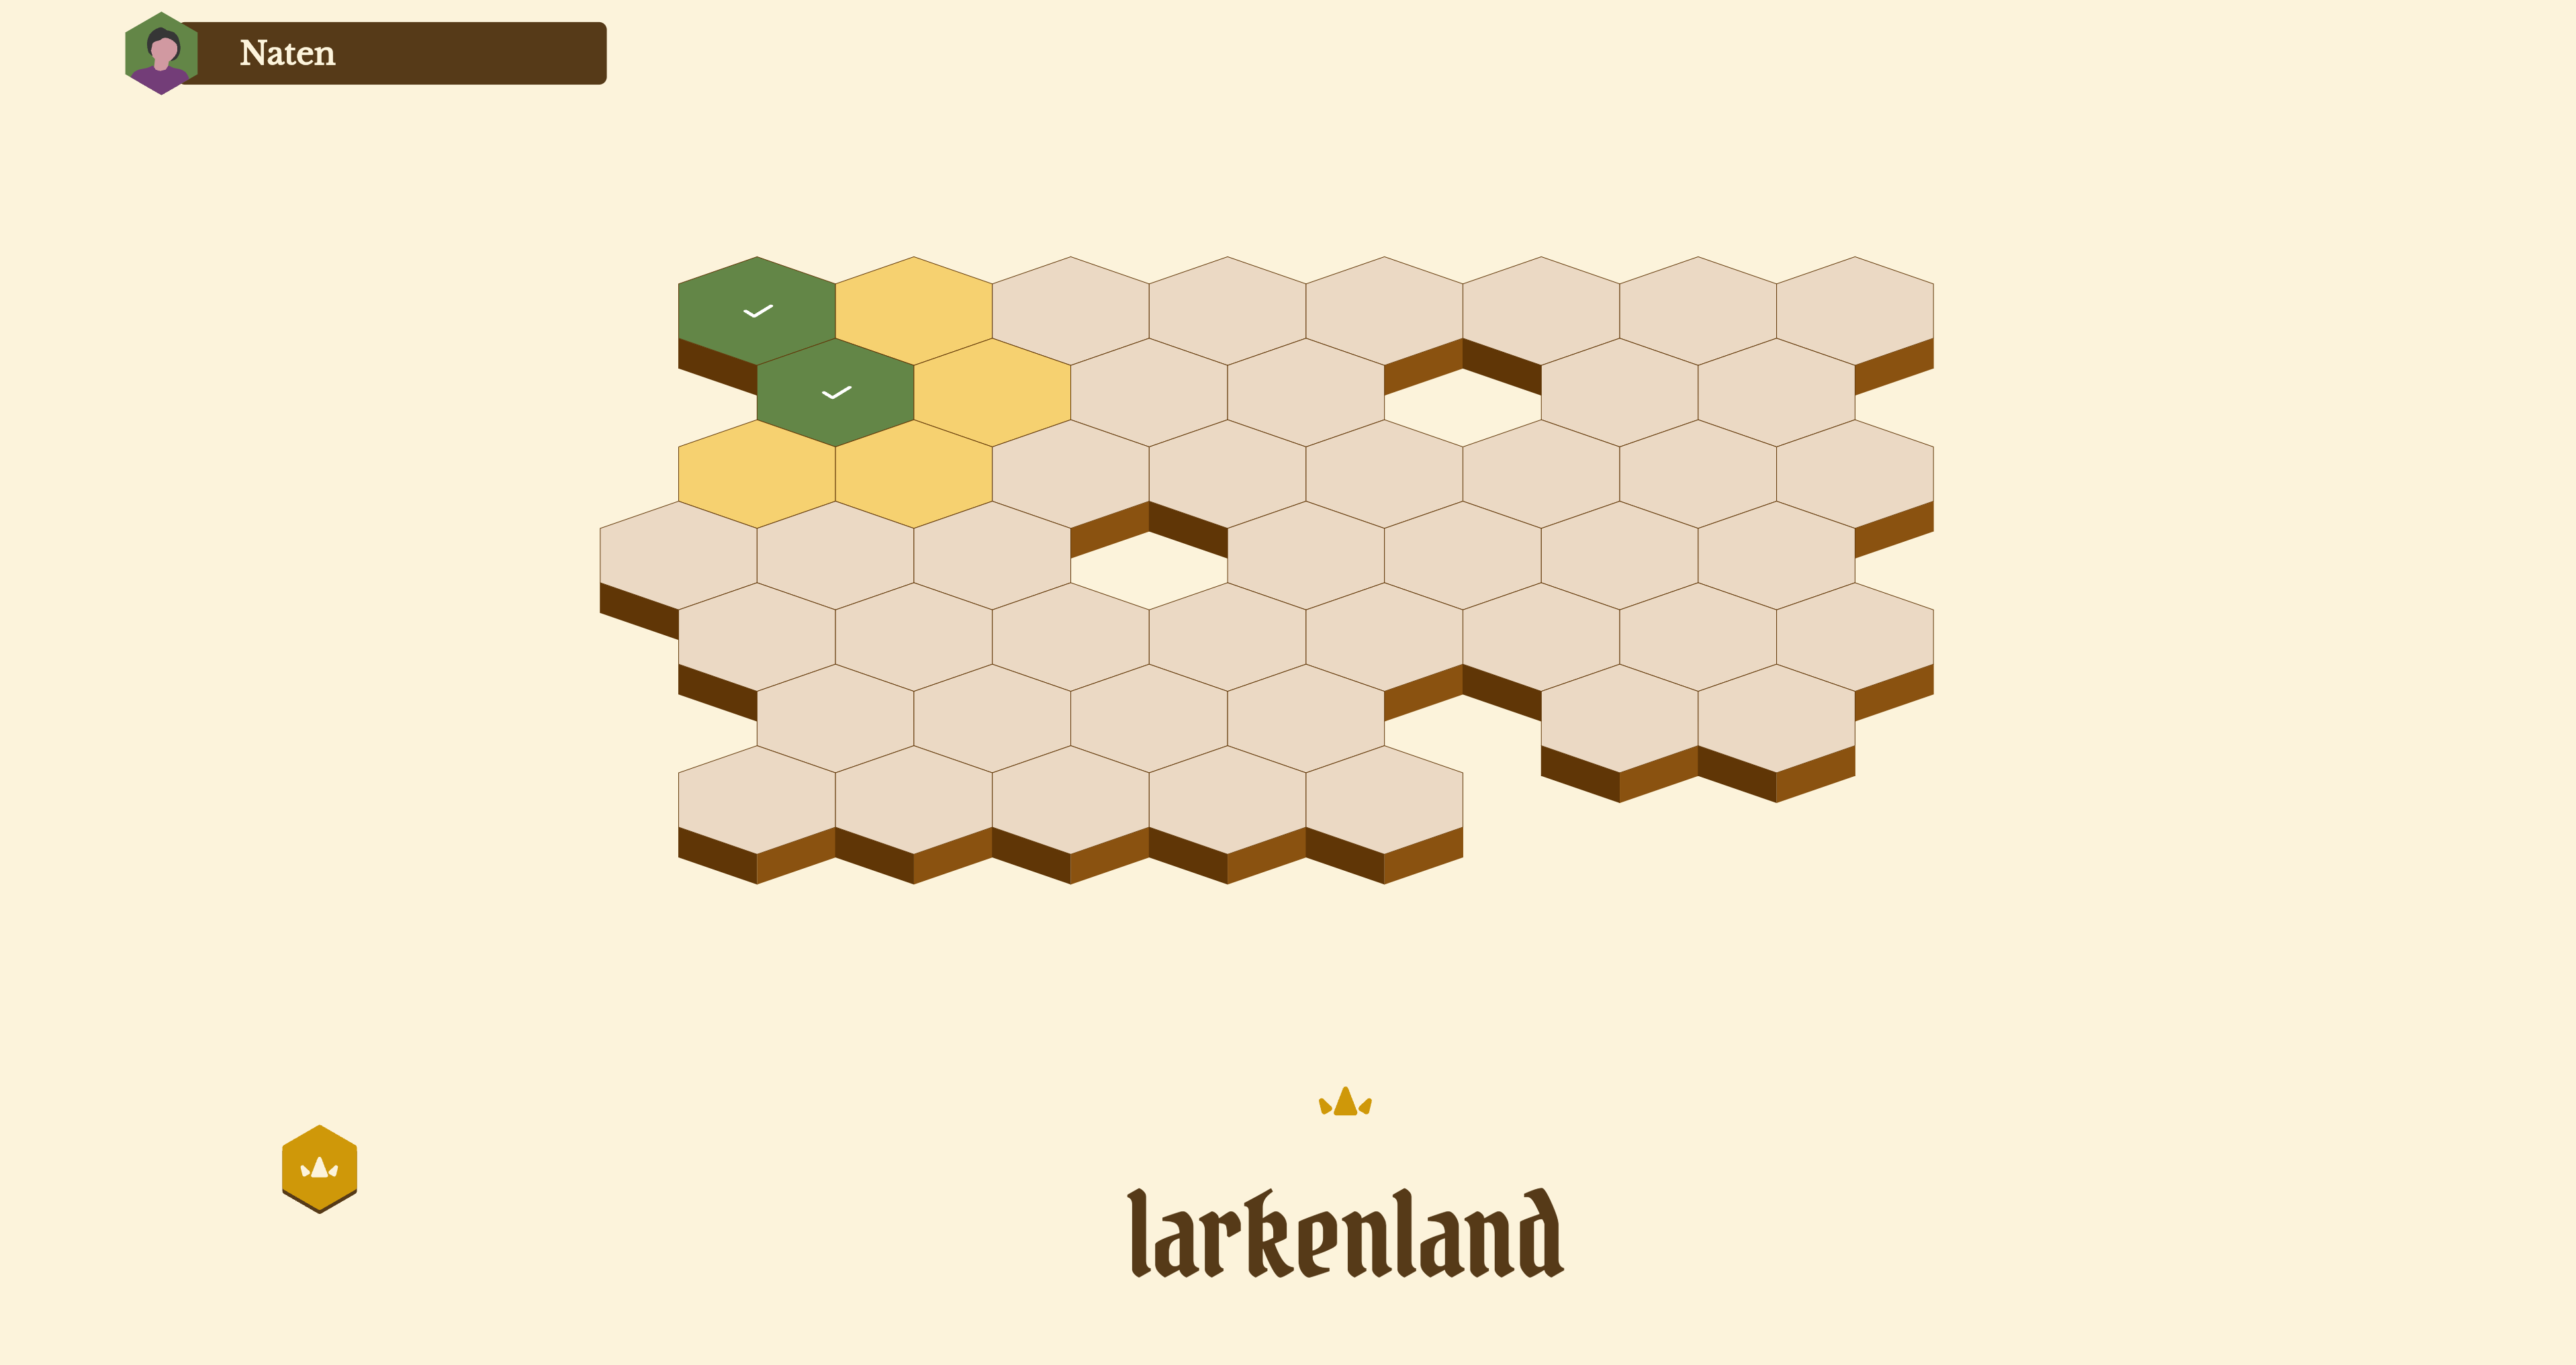
\includegraphics[width=0.85\textwidth]{figures/automatus_ui.png}
\caption{Screenshot of the Automatus interface from the pupil's perspective, showing the tile-based landscape through which learners navigate exercises.}
\label{fig:automatus_ui}
\end{figure}

On the six exercise-tool properties from Section \ref{sec:exercise-properties}, Automatus scores well on five of them. \textbf{Adaptivity} is handled in a specific way: rather than adjusting the difficulty of the exercises, Automatus adapts the goal time the child has to answer them. This is what the platform calls \textit{adaptive automatisation} as opposed to \textit{adaptive practice}, and it positions itself as one of the first platforms built around this distinction\footnote{\url{https://automatus.be/scholen/faq/wat-is-adaptief-automatiseren/}}. \textbf{Engagement} is supported by the map-and-tile structure, which gives children a visible sense of progress, and by response-time tracking that lets them compare their current attempt against their personal best, adding a layer of self-competition. \textbf{Feedback} is well-handled: when a child answers incorrectly, the exercise progress pauses and the platform shows a short explanation of the correct approach. \textbf{Accessibility} is excellent: Automatus runs in any browser and is also available as a tablet application, so it works on the devices schools and families actually have. \textbf{User friendliness} is equally strong: the interface is clean and intuitive enough that children can navigate it without adult help.

The one property where Automatus does not fully deliver is \textbf{personalisation}. The functional side is partially present: children can in some cases choose which exercises they want to work on, and the performance tracking gives a sense of individual progress. But the identity side is missing: there is no avatar, no personal profile beyond a name, no visual element that makes the tool feel like it belongs to the child rather than to the classroom. This is a minor gap in an otherwise very well-designed tool.

\subsection{Rekentuin}
Rekentuin (Math Garden) is a web-based arithmetic learning environment developed at the University of Amsterdam by Straatemeier, Klinkenberg, and van der Maas \cite{straatemeier2014mathgarden}. From the start it was built with a dual purpose: serving children as a practice platform and serving researchers as a scientific instrument for studying arithmetic development \cite{straatemeier2014mathgarden}. It has grown into one of the most widely used arithmetic tools in the Netherlands, with more than 400,000 primary school children practising on it \cite{brinkhuis2018learning}, and is now maintained and distributed as part of the Prowise Learn \cite{prowiselearn}.

The platform organises its content around a world map with multiple thematic islands, each representing a different mathematical domain. Children navigate between islands and work through exercises that range from basic addition to fractions and percentages. Figure~\ref{fig:rekentuin_ui} shows the main interface.

\begin{figure}
\centering
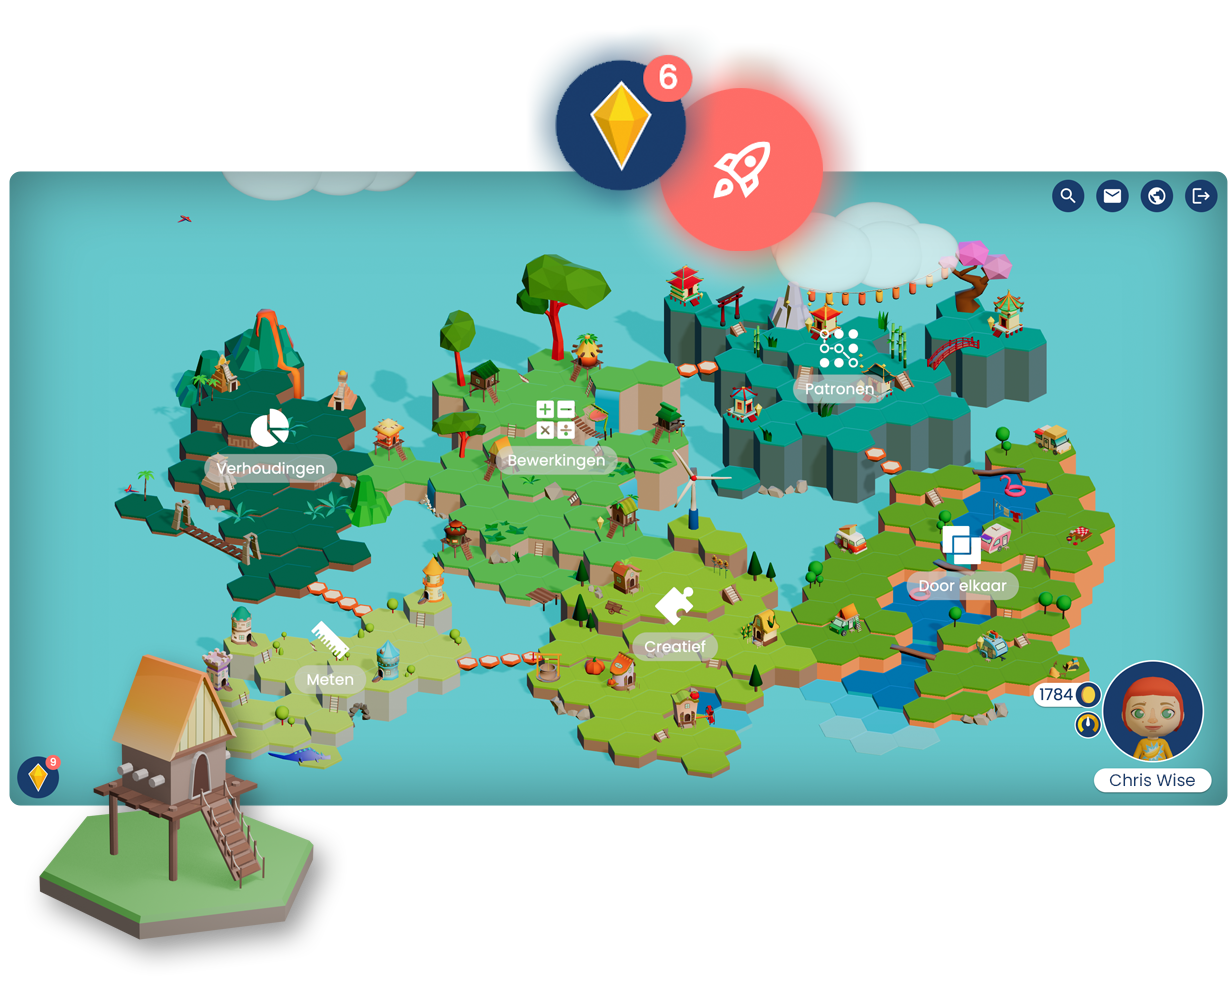
\includegraphics[width=0.85\textwidth]{figures/Rekentuin.png}
\caption{Screenshot of the Rekentuin interface from the pupil's perspective, showing the different continents from which learners can select different exercises.}
\label{fig:rekentuin_ui}
\end{figure}

On the six properties, Rekentuin delivers strongly across the board. \textbf{Adaptivity} is the cornerstone of the platform's design. Rekentuin's adaptive engine combines the Elo rating system with an item response model, continuously estimating how able each child is and how hard each item is, and then choosing items so that the child answers correctly with a probability of roughly 75\% \cite{klinkenberg2011computer}. Children can also choose between three difficulty levels within each game, adding a layer of self-regulation on top of the algorithm. \textbf{Engagement} is sustained through the island-based world, a variety of games across different mathematical topics, and a coin system: faster and more accurate answers earn more coins. The platform also highlights recommended games and ``super games'' based on the child's performance, gently steering practice toward areas that need attention. \textbf{Feedback} is immediate. Children see whether their answer was correct after each problem, and the coin reward provides a secondary signal of how well they performed relative to the time limit. \textbf{Personalisation} is where Rekentuin distinguishes itself most clearly from Automatus. The coins children earn are tied to an avatar that they can dress, decorate, and customise, giving every child a visible, personal identity within the platform. Combined with the personalised game recommendations and the self-selected difficulty levels, the experience feels suited to each individual. \textbf{Accessibility} is strong: Rekentuin runs in any web browser, including on mobile devices, and data from Klinkenberg et al. show that children completed roughly a third of their exercises outside school hours \cite{klinkenberg2011computer}, indicating that the platform is genuinely used at home as well as in the classroom. \textbf{User friendliness} is well-designed for the target age group, with large interactive elements, colourful visuals, and a navigation structure built around the world and islands that children understand intuitively.

At this point, a similar comparison to the one drawn for OpenSesame and PsychoPy in Section \ref{sec:research-tools} is useful. Figure~\ref{fig:exercise-tool-grid} evaluates both Automatus and Rekentuin against the six exercise-tool properties. Automatus falls just short on personalisation, while Rekentuin delivers on all six. These tools do exactly what they were designed to do. The question that follows is whether they can also serve the needs of researchers. That is the subject of the next section.

\begin{figure}
\centering
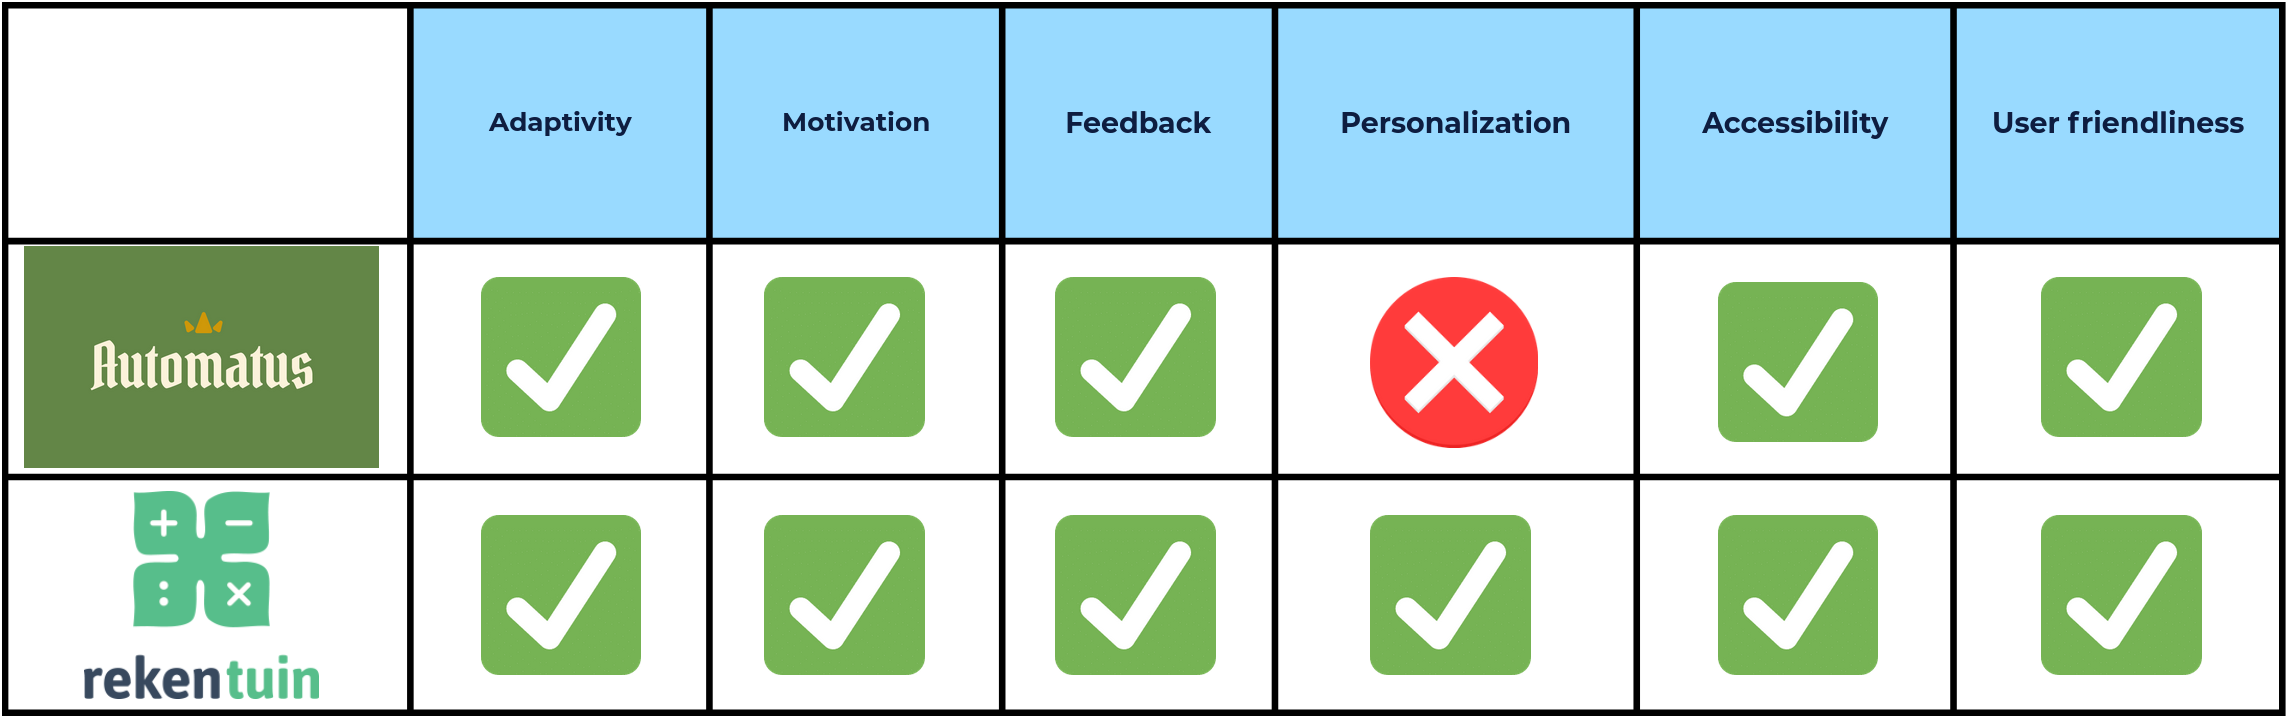
\includegraphics[width=0.85\textwidth]{figures/grid_exercise.png}
\caption{Automatus and Rekentuin evaluated against the six exercise-tool properties from Section \ref{sec:exercise-properties}. Both perform well across the board; Automatus falls slightly short on personalisation.}
\label{fig:exercise-tool-grid}
\end{figure}

\section{Why exercise tools alone are not the answer}
\label{sec:not-the-answer}
The previous section showed that Automatus and Rekentuin are excellent exercise tools. They are adaptive, engaging, well-designed, and genuinely enjoyed by children. A natural question follows: if these tools already solve the engagement and motivation problems that plague research tools, could they not simply be used for research as well?

To answer this, the same six research-tool properties from Section \ref{sec:research-properties} can be applied to both platforms. The result, summarised alongside the exercise-tool evaluation in Figure~\ref{fig:combined-grid}, shows a clear pattern. On three of the six research properties, both tools perform well. On the other three, they fall short in ways that matter.

The three properties that hold up are straightforward. \textbf{Reproducibility} is well-supported: once a teacher has configured a set of exercises for a class, that configuration is saved and can be reused next semester without effort. \textbf{Reliability} is equally strong. Both Automatus and Rekentuin are mature, commercially maintained products used daily by hundreds of thousands of children. They are stable, they do not crash mid-session, and they behave consistently across devices. \textbf{Ease of setup} is, unsurprisingly, a strength rather than a weakness. Both tools were built for teachers, not programmers. Setting up a class, assigning exercises, and managing student progress is done entirely through a graphical dashboard with no code involved.

The problems emerge in the remaining three properties. \textbf{Data tracking} is the first issue. Both platforms collect data on student performance, and teachers can see summaries of accuracy and progress over time. But the level of detail is not what a researcher needs. Arithmetic research requires the exact response time for every individual trial, the precise answer the child gave (not just whether it was correct), and ideally the timestamp of every screen transition. These fine-grained data points are what allow researchers to distinguish, for example, between a child who retrieved a fact from memory in under two seconds and one who calculated the answer in five. Exercise tools log enough to inform a teacher; they do not always log enough to inform a study.

\textbf{Experimental control} is the second and arguably most fundamental problem. As discussed in Section \ref{sec:research-properties}, controlled experiments depend on the researcher being able to dictate what each participant sees and under what conditions. Exercise tools are designed around a partly opposite principle: they are built to give children autonomy, with the system adapting on its own and the teacher setting broad goals rather than trial-by-trial sequences. Some features can be configured by the teacher, and it is not impossible to get two children to see the same set of exercises. But for the kind of fine-grained control a research design typically needs (disabling specific features for a single group, forcing a fixed item sequence, switching off adaptivity while keeping everything else the same) the platforms simply were not designed with this in mind, and the level of control an OpenSesame-style tool offers is out of reach.

\textbf{Flexibility} is the third gap, and it is closely tied to the previous one. As also discussed in Section \ref{sec:research-properties}, flexibility in a research context is the ability to set up a wide range of experimental designs without rebuilding the tool. The configuration options exercise tools expose are designed for pedagogical goals, not experimental ones. A researcher who wants to swap the adaptive algorithm for a different one, introduce a new kind of task, or restructure the session into multi-block sequences with custom rules between blocks has no way to express any of that within the platforms. The kind of flexibility a programming language offers is absent, and the graphical interface itself was never built to support the structured designs that some research studies require.

Figure~\ref{fig:combined-grid} brings both evaluations together. The research-tool properties are on the left, the exercise-tool properties on the right. Automatus and Rekentuin fill the right side almost entirely with green. The left side tells a different story: reproducibility, reliability, and ease of setup are covered, but data tracking, experimental control, and flexibility are not. Exercise tools, on their own, are not the answer. But the qualities they bring to the table are exactly the qualities that Chapter \ref{chp:background} identified as missing from research tools. The next section brings all four tools and all twelve properties together to make this gap fully visible.

\begin{figure}
\centering
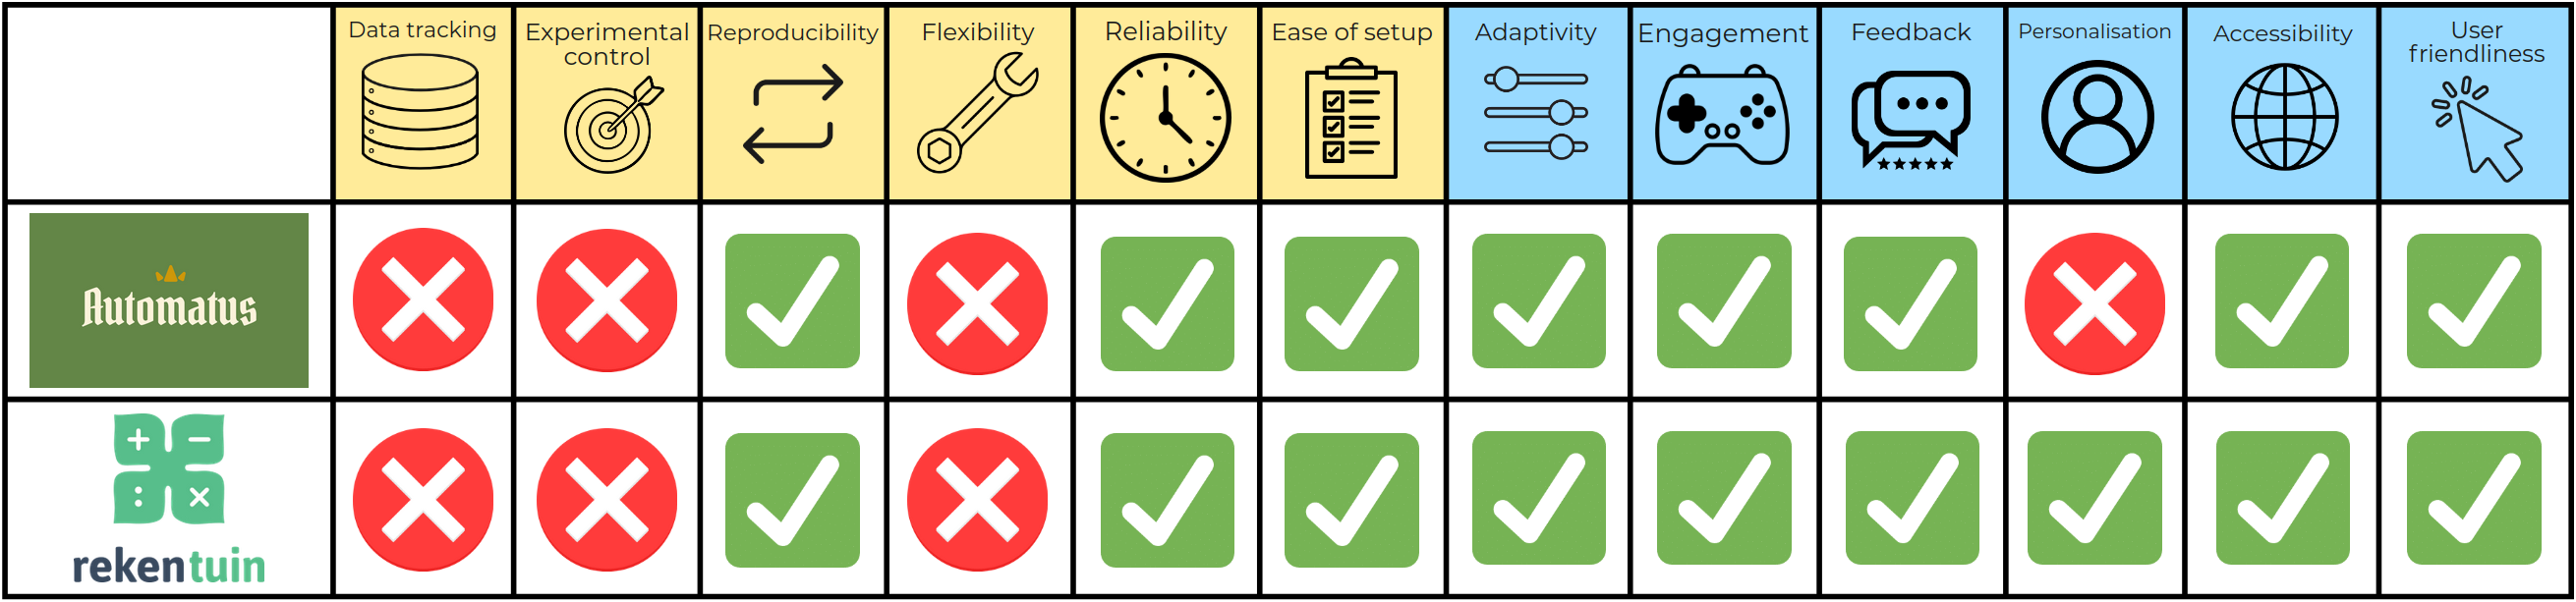
\includegraphics[width=0.85\textwidth]{figures/grid_exercise_research.png}
\caption{Combined comparison of Automatus and Rekentuin against both the exercise-tool properties (Section \ref{sec:exercise-properties}) and the research-tool properties (Section \ref{sec:research-properties}). Both tools excel on the exercise side but fall short on data tracking, experimental control, and flexibility.}
\label{fig:combined-grid}
\end{figure}


\section{The gap: no existing tool covers both sides}
The previous sections built up the comparison piece by piece. Section \ref{sec:research-tools} evaluated OpenSesame and PsychoPy on the research-tool properties, Section \ref{sec:exercise-tools} evaluated Automatus and Rekentuin on the exercise-tool properties, and Section \ref{sec:not-the-answer} tested whether exercise tools could also serve as research tools and found that they could not. The one combination left to make explicit is the reverse: how do the research tools score on the exercise-tool properties?

Section \ref{sec:shared-limitations} answered this question. OpenSesame and PsychoPy were not built to be exercise tools, and they offer none of the six properties from Section \ref{sec:exercise-properties} out of the box. There is no built-in adaptivity, no gamification, no avatar system, no child-friendly login. All of these could in theory be added, but only by writing them from scratch in Python, which brings the researcher straight back to the same programming wall that already made ease of setup the weakest point on the research side.

Figure~\ref{fig:full-grid} brings everything together. All four tools are evaluated against all twelve properties: the six research-tool properties on the left, the six exercise-tool properties on the right. The pattern is now fully visible. Automatus and Rekentuin fill the exercise columns with green but leave gaps in the research columns. OpenSesame and PsychoPy do the reverse. Each tool excels at what it was designed for. None covers both sides.

\begin{figure}
\centering
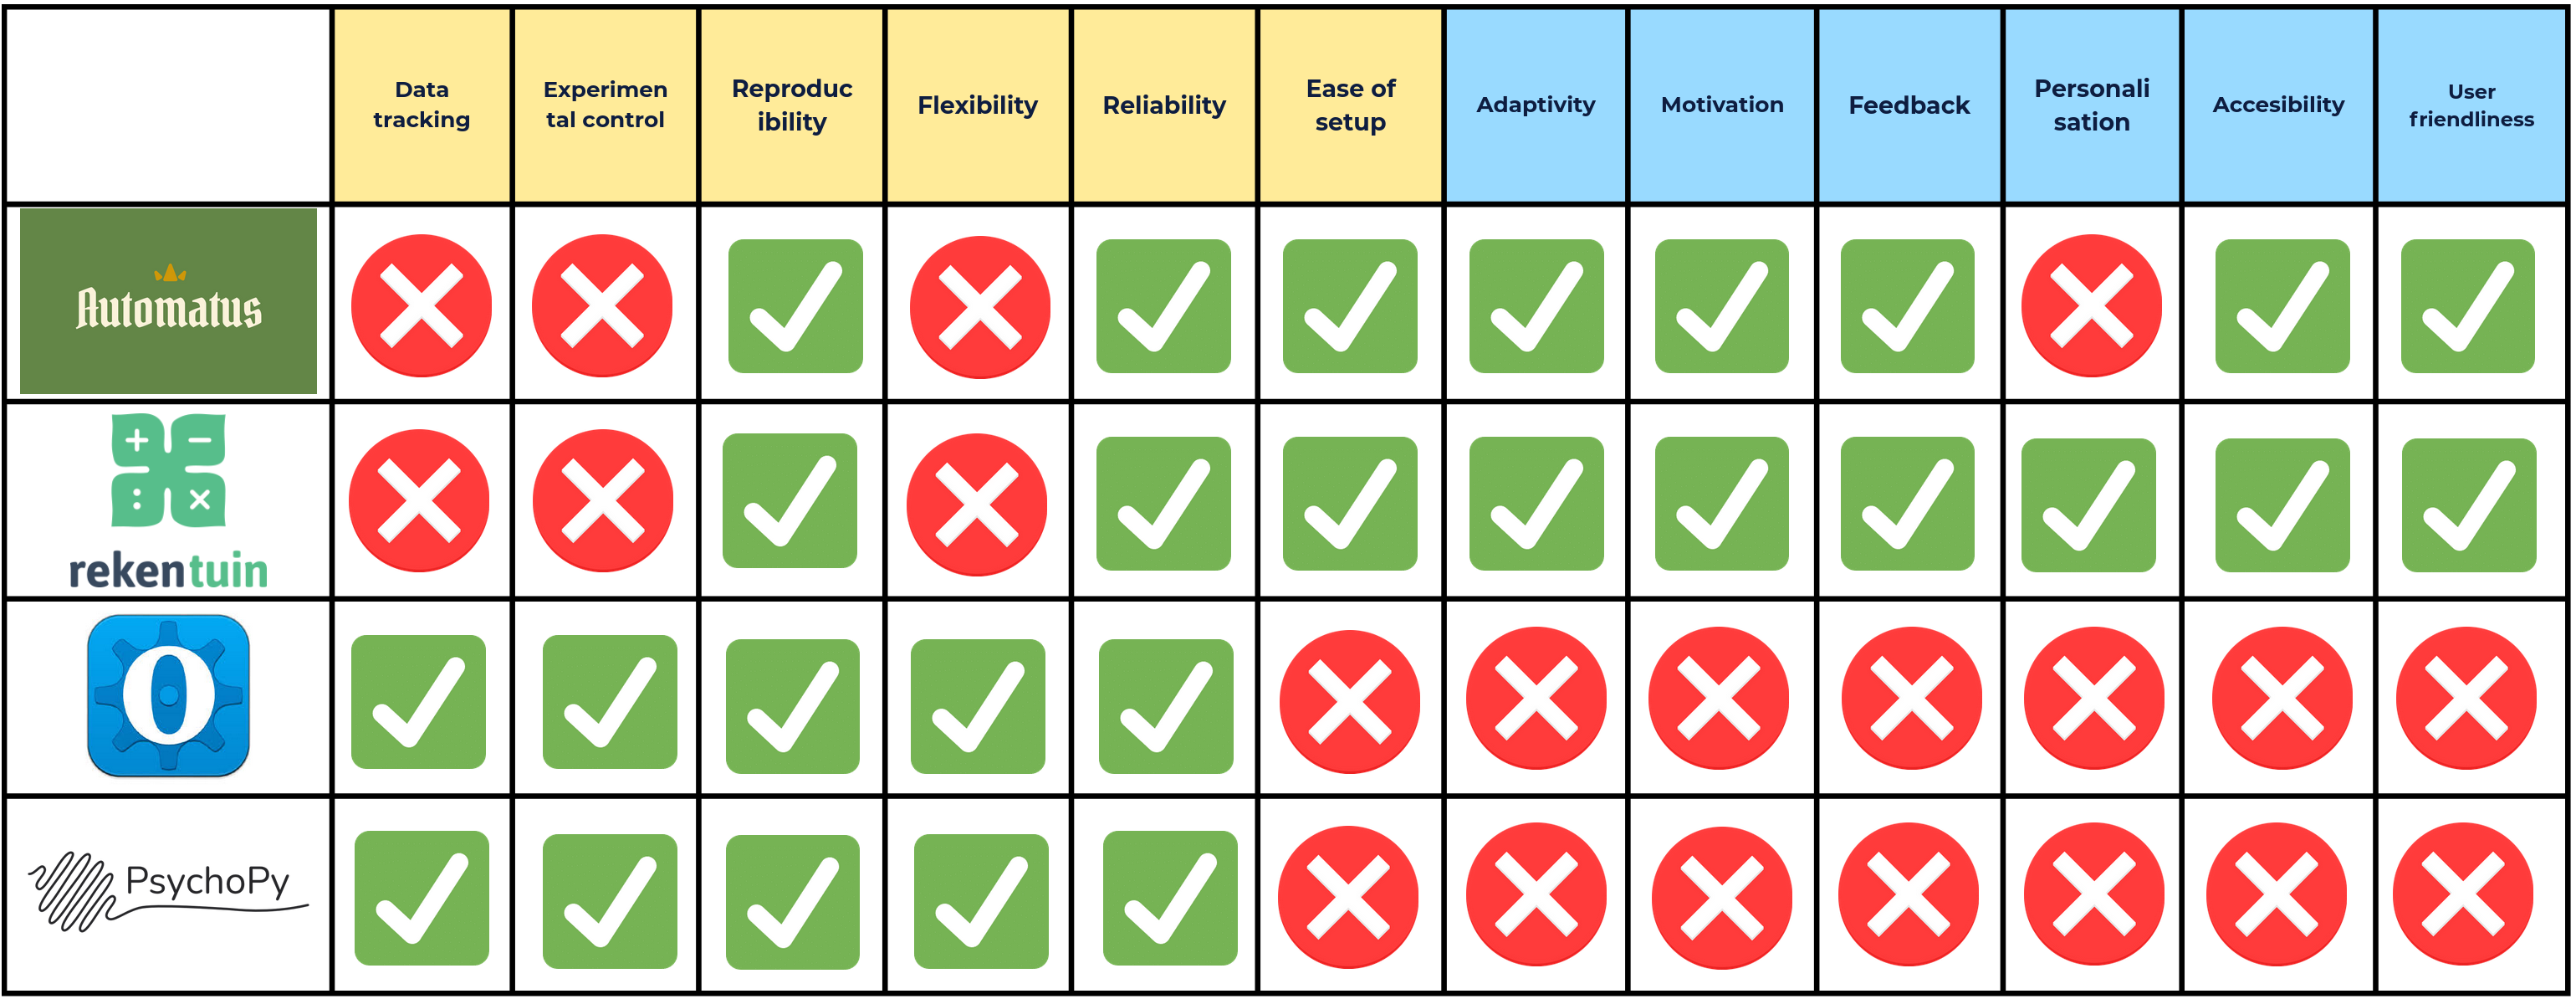
\includegraphics[width=0.85\textwidth]{figures/grid.png}
\caption{Full comparison of all four tools against the twelve properties defined in Sections \ref{sec:research-properties} and \ref{sec:exercise-properties}. Exercise tools (top) score well on exercise properties but lack key research properties. Research tools (bottom) score well on research properties but offer none of the exercise-tool qualities.}
\label{fig:full-grid}
\end{figure}

This is not a criticism of any of these tools individually. Each was built for a specific purpose and serves that purpose well. But for a researcher who wants to run a controlled experiment in a classroom, with children who stay motivated across multiple sessions, using a tool that feels familiar rather than foreign, there is currently no option that works. That gap is formalised in the next chapter.
\include{chapters/problem_statement}
% !TeX root = ../thesis.tex
\chapter{RekenRangers}
\label{chp:rekenrangers}
The previous chapters identified a gap between classroom exercise tools and controlled research software, and Chapter \ref{chp:problem-statement} formalised that gap as a problem statement. This chapter describes RekenRangers\footnote{Although the application is officially named \textit{RekenRangers}, the English name \textit{MathRangers} may also be used throughout this thesis for readability and convenience.}, the platform built to address it. RekenRangers is a web-based arithmetic learning tool designed for primary school children aged 7 to 11. It is built to function both as a daily classroom exercise tool and as a configurable research instrument, so that the same platform children use to practise arithmetic can also serve as the environment in which researchers run controlled experiments.

The platform is hosted on a KU Leuven server and accessible through any modern web browser at \texttt{https://rekenrangers.cs.kuleuven.be/}, which means it runs on the laptops, tablets\footnote{RekenRangers runs in any tablet browser, but the interface has not been specifically optimised for tablets, and there is currently no tablet application. Both are possible directions for future work.}, and Chromebooks that schools already have without requiring any installation. The back-end is written in Python using the Flask web framework \cite{grinberg2018flask}, with a MySQL database for persistent storage. The front-end uses HTML, CSS, and JavaScript, with the Bootstrap library for responsive layout. The full codebase is maintained in a private GitHub repository.\footnote{The author of this thesis intends to set an open-source license on the repository in the future, so that the platform can be reused, extended, and inspected by other researchers.}

This chapter begins by describing the design process and the decisions that shaped the platform at a high level, then walks through the tool's approach to each of the twelve properties identified in Chapters \ref{chp:background} and \ref{chp:exercise-tools}.

\section{Design process and guiding principles}
RekenRangers was not designed in isolation. Building a tool that needs to work for children, teachers, and researchers at the same time is hard to do without input from all three groups, and the design process was set up to make at least some of that input possible. While the project did not involve frequent direct meetings with teachers or children, advice was sought from these groups at key moments, and the design was continuously discussed with the researchers who would eventually use the tool in their own studies. Research in educational technology has consistently shown that involving stakeholders early and continuously in the design process leads to tools that are more likely to be adopted and that better fit the needs of the people who will actually use them \cite{cumbo2022participatory}.

The core development, both back-end and front-end, was carried out by the author of this thesis. Design decisions, however, were shaped through continuous collaboration with several key partners. Throughout the project, the author's supervisor, Prof. Dr. Tom Schrijvers, provided guidance on the overall direction of the work and feedback on its development. On the educational-research side, the co-supervisor of this thesis, Elien Bellon, contributed both the scientific grounding for the platform's features and a concrete benchmark study to replicate, drawing on her own research on metacognitive monitoring in arithmetic \cite{bellon_more_2019, bellon2020, bellon2021}. Two master's students in pedagogical sciences at KU Leuven, Eline T'joen and Kiara Willems, were also closely involved, since their own theses depended on using RekenRangers in classroom settings. Their involvement meant that design decisions were tested against real use cases from the start: if a feature did not make sense to someone planning a study with third-graders, it was reworked. A final, less direct source of input was the set of existing tools discussed in Chapters \ref{chp:background} and \ref{chp:exercise-tools}. These tools served a dual role. Rekentuin and Automatus provided models for what a child-friendly arithmetic tool looks and feels like, from adaptive difficulty to avatar systems to coin-based reward structures. OpenSesame and PsychoPy provided a clear reference for the kinds of experimental control and data logging a research tool must offer, but they also provided a vivid image of what happens when engagement is not a priority. The black-screen, stimulus-response experience that characterises most experiments built in these tools (see Figure~\ref{fig:black_screen}) was a constant reminder of what RekenRangers needed to avoid.

This combination of perspectives shaped two core principles that guided the design throughout.

The first was that the replication of the Bellon et al. study \cite{bellon_more_2019} had to be possible. This study, which investigates the relationship between metacognitive monitoring and arithmetic performance in children, lived in the back of the author's mind throughout development: it was a concrete example of a study that had already been run in OpenSesame and that the researchers involved had found difficult to set up there. It was not used as a checklist that every feature was tested against, but it acted as a recurring reference point that kept the development grounded in a real research need rather than in abstract feature lists.

The second was a matter of audience. RekenRangers needed to be configurable by people who do not write code and feel like a game to the children using it. These are essentially restatements of the central goals identified in Chapters \ref{chp:background} and \ref{chp:exercise-tools}, but they were treated as design principles in their own right: every screen, every flow, and every configuration option was evaluated against whether it served a non-programming researcher on one side and a seven-year-old on the other.

Generative AI tools were used during development to assist with specific implementation tasks such as generating boilerplate code and debugging. All architectural decisions, feature design, and user interface design were made by the author in collaboration with the partners described above.

The following section describes how each of the twelve properties from Chapters \ref{chp:background} and \ref{chp:exercise-tools} was addressed in the design and implementation of RekenRangers.

\section{Approach: design decisions per property}
This section walks through each of the twelve properties from Chapters \ref{chp:background} and \ref{chp:exercise-tools} and describes how RekenRangers addresses them. The research-tool properties are discussed first, followed by the exercise-tool properties.

\subsection{Data tracking}
\label{sec:data-tracking}
Section \ref{sec:research-properties} defined data tracking as the most basic requirement of any research tool: the tool must record what happens, completely and automatically. In RekenRangers, every exercise completed by every child produces a full data record that is stored in the database. The level of detail was determined in close collaboration with Eline T'joen, Kiara Willems, and co-supervisor Elien Bellon, to ensure that the logged data would be sufficient for the kinds of analyses that arithmetic research requires.

Each record captures the full context of a single exercise: who answered, the operation and operands presented, the answer given, whether it was correct, and the response time. The record also includes the difficulty level, whether the timer was visible, the child's current Elo rating and the change in rating produced by that exercise, and the difficulty zone the child was in at the time. When the metacognitive self-assessment is enabled, the confidence judgement is logged together with a calibration field capturing whether the self-assessment matched the actual outcome. Response times are recorded separately for the exercise, the confidence judgement, and the feedback screen, which lets researchers analyse not just what children answered but how long they spent on each phase of the trial. The complete list of fields is given in Appendix~\ref{app:data-fields}.

This data is accessible in two ways. The teacher dashboard, when a student is selected from the group overview, shows the full list of exercises that student has completed, at a level of detail aimed at the teacher rather than at the researcher. For research purposes, the group screen offers an export function that generates a single CSV file containing every exercise completed by every student in the group. This file can be opened directly in Excel or imported into statistical software for analysis. The export is designed to require no preprocessing: each row is one exercise, each column is one variable, and no manual cleaning or restructuring is needed before the data can be used.

\subsection{Experimental control}
\label{sec:experimental-control}
Experimental control is the property that most clearly separates a research tool from a classroom tool. Section \ref{sec:research-properties} defined it as the ability to dictate precisely what each participant sees and under what conditions, so that the researcher can isolate the variables they are studying. In RekenRangers, experimental control is implemented through a layered settings system in the teacher dashboard, where each group of children can be configured independently.

The first layer covers the general exercise settings. For any group, the teacher or researcher can choose which arithmetic operations are available, how difficulty is determined (adaptive, fixed, or chosen by the child), whether a timer is shown, and whether metacognitive self-assessment prompts are enabled. These settings are sufficient for classroom use and for simple studies where the main concern is controlling what type of exercises children see. The full list of configurable settings is provided in Appendix~\ref{app:group-settings}.

The second layer covers the research settings (Figure~\ref{fig:research-settings}), where the experimental control becomes precise. The most important option here is \textit{research mode}. When research mode is enabled, the interface changes in ways that are invisible to the child but critical for the researcher. Mouse interaction is disabled entirely, so that all input happens through the keyboard. Buttons and interface elements that are not essential to the exercise flow are hidden or deactivated, reducing the chance that a child accidentally navigates away from the task or gets distracted by something outside the experiment. Several pieces of interface text are also adjusted: in normal mode some labels offer the child additional options that are no longer available in research mode, so the corresponding text is replaced with a research-mode equivalent. In short, research mode strips the interface down to what the experiment requires and nothing more.

Within the research settings, a set of item generation rules gives the researcher fine-grained control over which exercises can appear. Identical exercises can be blocked from appearing twice within the same session. Tie problems, where both operands are the same number (such as \(4+4\) or \(7 \times 7\)), can be excluded because they are known to be solved through different processes than non-tie problems \cite{campbell2002tie}. Exercises that produce the same result can be prevented from appearing consecutively. Commutativity can be enforced, so that \(3 \times 7\) and \(7 \times 3\) are registered as the same exercise. The position of the larger operand can be balanced across trials to prevent children from developing a position bias. Beyond these structural rules, the researcher can define exclusion lists for specific operand values and results, for example excluding 0, 1, or 11. A fixation screen can also be enabled before each exercise, which is standard practice in reaction-time research to ensure the child is focused before the stimulus appears.

Effort also went into ensuring that children cannot inadvertently break the experimental flow. In research mode, there is no way to skip an exercise, navigate to the puzzle screen mid-session, or exit the exercise sequence (except through browser actions). Answers are constrained to valid numerical input, and the interface enforces a fixed progression from exercise to self-assessment to feedback to the next exercise. In a classroom with twenty children working simultaneously and no researcher behind each screen, these details are the difference between clean data and a session that has to be discarded.

The combination of the general settings and the research-specific controls means that a researcher can configure two groups within the same classroom to see identical exercises but with different feedback conditions, or the same feedback conditions but with different difficulty settings, without writing any code.

\begin{figure}
\centering
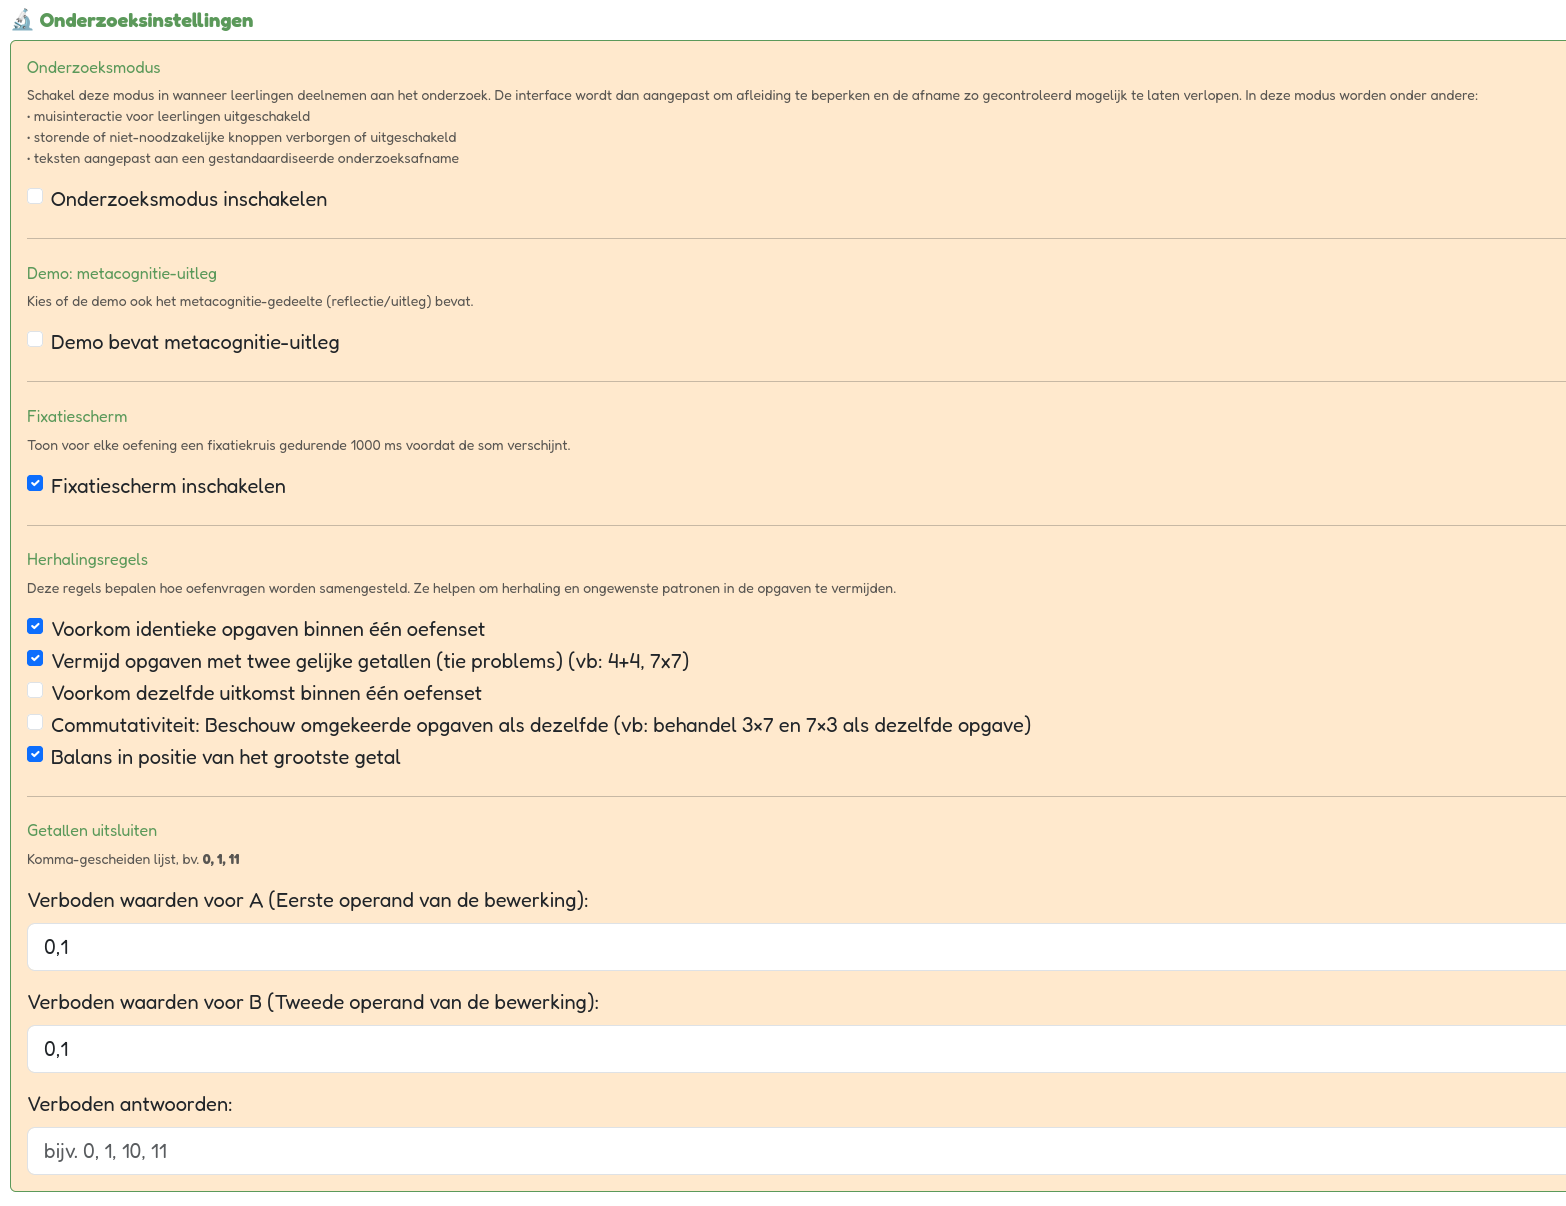
\includegraphics[width=0.85\textwidth]{figures/research-settings-new.png}
\caption{Research settings panel. Researchers can enable research mode, configure item generation rules (e.g.\ tie-problem exclusion, commutativity), define operand exclusion lists, and enable a fixation screen.}
\label{fig:research-settings}
\end{figure}

\subsection{Reproducibility}
Section \ref{sec:research-properties} defined reproducibility as the ability to save, share, and rerun the exact configuration of an experiment. RekenRangers supports this through a JSON-based export and import system, an idea suggested by Tijs Bellefroid. Every setting described in the previous section, from the operation selection to the research-mode rules to the exclusion lists, can be exported to a single JSON file with one click. A second researcher who wants to replicate the study can import that file into their own group, and every setting is restored exactly as it was. Sharing an experimental setup is then as simple as sharing a file.

One important consideration: two children configured with the same settings will not necessarily see the same sequence of exercises. The settings constrain which exercises are allowed, but the choice of which specific exercise comes next is partly random within those constraints. This is reproducibility at the level of experimental conditions, not at the level of literal trial-by-trial identity, which is the level that matters for between-group comparisons.

\subsection{Flexibility}
\label{sec:flexibility}
Flexibility, as defined in Section \ref{sec:research-properties}, is about whether a tool can support a wide variety of experimental designs without requiring the researcher to modify the underlying code. The settings system described in the previous sections already contributes to this: the ability to configure operations, difficulty modes, metacognitive prompts, timer settings, and item generation rules means that a single installation of RekenRangers can host studies with very different designs. But settings alone are not enough. Most research designs in educational psychology do not consist of a single uniform block of exercises. They involve phases: a warm-up, a main task, a break, a post-test, sometimes with different conditions across phases.

RekenRangers addresses this through an exercise sequence system. A sequence consists of multiple blocks, each with its own settings for the number of exercises, the operation, the difficulty mode, and whether metacognitive prompts are enabled. A researcher can, for example, configure a sequence that starts with 10 easy addition exercises as a warm-up without self-assessment, followed by three blocks of 15 adaptive exercises with metacognitive prompts, and a final block of 10 fixed-difficulty exercises as a post-test. Each block is independently configurable, and blocks can be added, edited, reordered, or removed through the dashboard. The research settings (research mode, exclusion rules, fixation screen) apply to the entire sequence rather than per block, which ensures consistency across phases.

The teacher dashboard also provides tools for managing progress through a sequence. The progress of individual students or the entire group can be reset to the beginning of the first block, which is useful when a session needs to be restarted or when the same sequence is used across multiple days. On the student side, a visual progress indicator shows the child where they are in the sequence, and how many blocks remain before they can puzzle. Figure~\ref{fig:sequence-screen} shows the sequence configuration screen in the teacher dashboard.

\begin{figure}
\centering
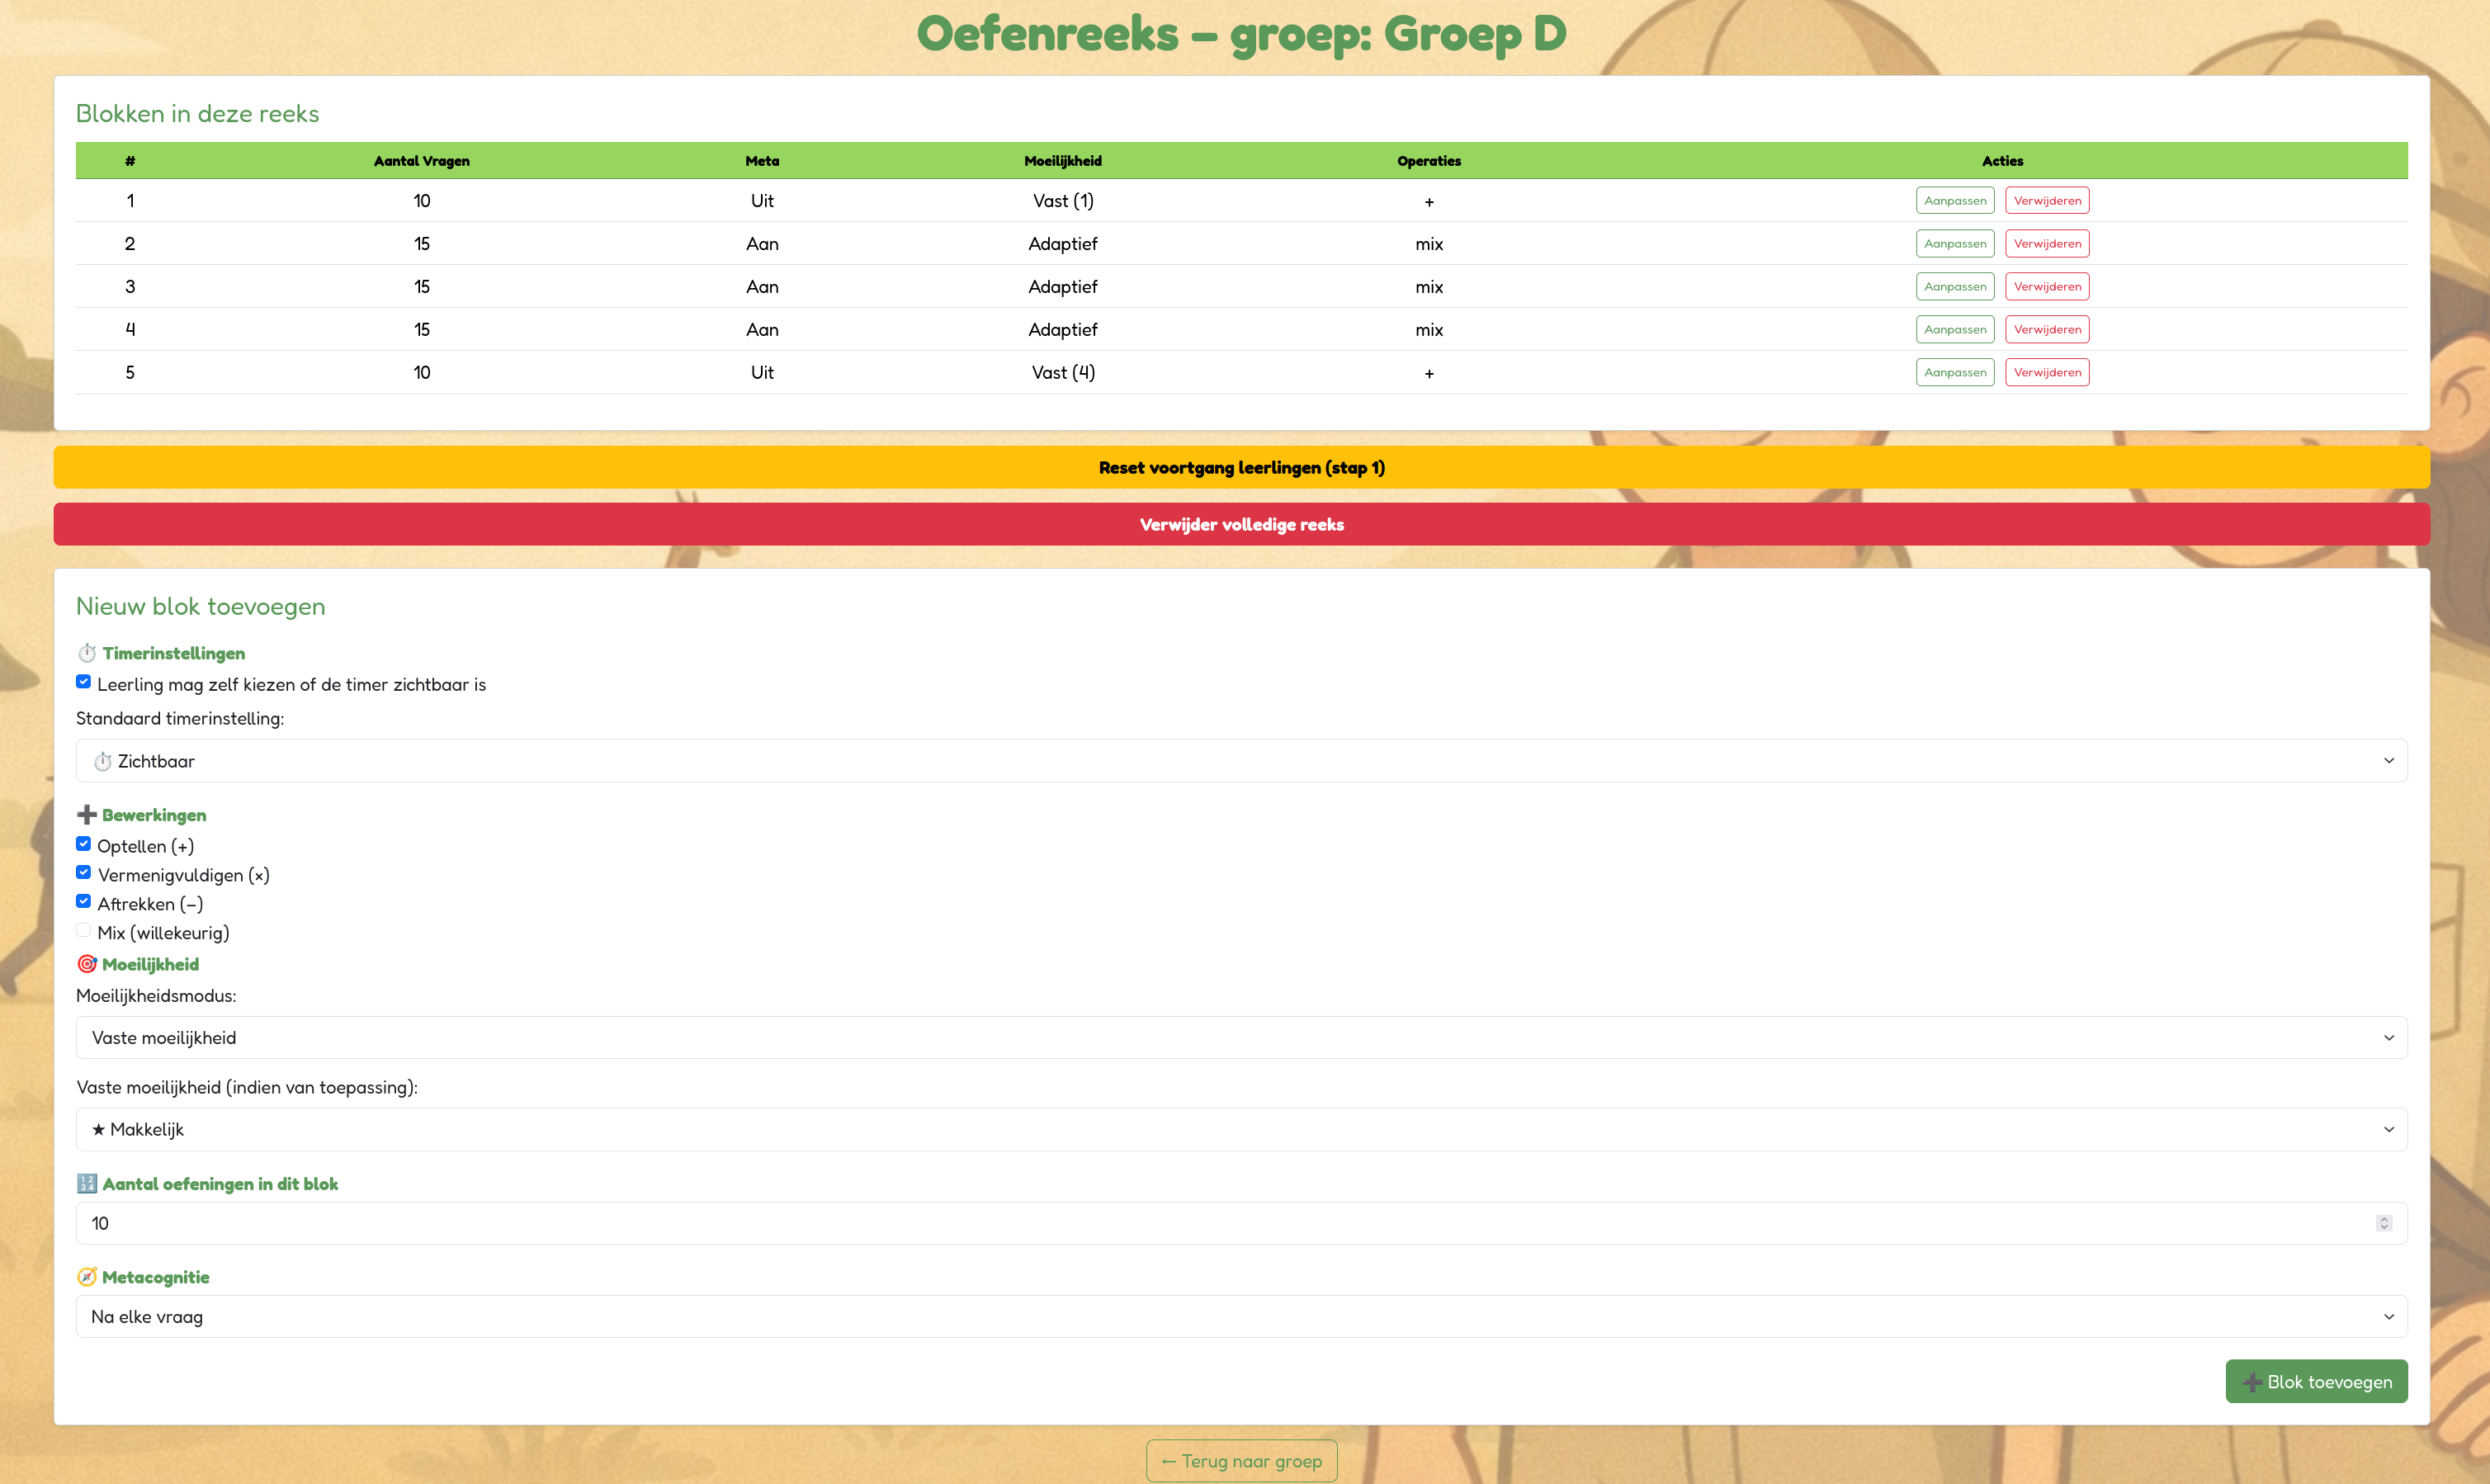
\includegraphics[width=0.8\textwidth]{figures/sequence-screen-new.png}
\caption{The exercise sequence configuration screen. Each row represents a block with its own settings. Blocks can be added, edited, or removed, and student progress can be reset individually or for the entire group.}
\label{fig:sequence-screen}
\end{figure}

The sequence system tries to make RekenRangers more flexible than any of the exercise tools discussed in Chapter \ref{chp:exercise-tools}, and for the kinds of studies it was designed to support, the configurability is sufficient. It does not, however, match the flexibility of a general-purpose programming environment: studies that require trial structures outside the block model, custom adaptive algorithms, or stimulus types beyond arithmetic cannot be expressed within the current tool. This reflects what Lidwell, Holden, and Butler call the ``flexibility--usability tradeoff'': ``as the flexibility of a system increases, the usability of the system decreases'' \cite{lidwell2010universal}. The limits it imposes on RekenRangers are discussed further in Section \ref{sec:limitations}.

\subsection{Reliability}
Section \ref{sec:research-properties} described reliability as having two dimensions: the tool must be robust, stable, and precise in its measurements, and it must keep running under real-world conditions on the kind of hardware schools actually have. RekenRangers addresses both.

On the robustness side, the platform is hosted on a KU Leuven server running inside a containerised environment using Podman and Docker, which isolates the application from the underlying system and makes deployment reproducible and stable. The MySQL database ensures that all data is persistently stored the moment an exercise is completed. If a child's browser crashes mid-session, or if the school's internet drops briefly, the data from every exercise completed up to that point is safe and does not need to be re-collected. The child can log back in and continue from where they left off without losing progress.

On the measurement side, response times are handled in JavaScript on the child's local machine. The timer for an exercise starts when the browser has fully rendered the stimulus on screen, and stops when the child submits their answer. This means that response times reflect actual thinking time rather than being inflated by network latency or server processing delays. The same local timing approach is used for the self-assessment and feedback phases.

The platform was tested across a range of common browsers and some small pilot sessions during development. A more substantial test of how RekenRangers holds up under real classroom conditions is provided by the experiment described in Chapters \ref{chp:experimental-setup} and \ref{chp:results}, with its outcomes discussed in Chapter \ref{chp:discussion}. It is worth noting up front, however, that RekenRangers has not been benchmarked against the kind of formal millisecond-level timing study that has been carried out for tools like PsychoPy \cite{bridges2020timing}.

\subsection{Ease of setup}
The design principle that no feature should require programming knowledge runs through the entire teacher and researcher experience. Every setting discussed in the previous sections, from operation selection to research mode configuration to exercise sequence design, is controlled through dropdown menus, checkboxes, toggle switches, and input fields in a graphical dashboard. There are no configuration files to edit, no scripts to write, and no command-line tools to learn. A researcher who wants to set up a study with three blocks of adaptive multiplication exercises with metacognitive prompts and tie-problem exclusion can do so in a few minutes without ever leaving the browser.

The exercise sequence system in particular benefits from its visual presentation. Each block in a sequence is displayed as a row in a table showing its key settings at a glance, which makes it easy to verify that the experimental design matches the intended protocol. Blocks can be added, reordered, or removed with a single click, and changes are saved immediately. This kind of visual configuration is one of the clearer differences with the research tools discussed in Chapter \ref{chp:background}, where similar functionality would typically require writing and maintaining a Python script.

The teacher and researcher dashboard was designed to be self-explanatory, but for users who need additional guidance a comprehensive manual has been developed that explains every feature and setting in detail. The manual was drafted with the help of generative AI to speed up the writing, and then checked manually to make sure every described feature behaves as written. It is available both within the platform itself\footnote{\url{https://rekenrangers.cs.kuleuven.be/static/handleiding_leerkracht.html}} and as a standalone document included in Appendix~\ref{app:teacher-manual}. A video walkthrough is also available.\footnote{\url{https://youtu.be/jeK2u8FNoPU}}

There is also room for improvement on this front, for example a preview of what the child will see given the current configuration, or a visual timeline of the exercise sequence rather than a table. The current setup interface is functional but does not yet scale with the number of options it now supports, which is one of the limitations of the platform discussed further in Section \ref{sec:limitations}.

\subsection{Adaptivity}
\label{sec:adaptivity}
A core requirement identified in Section \ref{sec:exercise-properties} is that exercises should match the child's current ability level. RekenRangers implements this through an adaptive difficulty system inspired by the Elo rating principle, informed by the work of Klinkenberg et al. on the adaptive engine behind Rekentuin \cite{klinkenberg2011computer}. The system described below was developed in collaboration with Eline T'joen and Kiara Willems.

The central idea is that each child maintains a numerical rating that reflects their estimated skill level. This rating starts at 450 on a scale from 0 to 1000 and is updated after every exercise using the standard Elo update rule:

\begin{equation}
\theta'_j = \theta_j + K(S{ij} - E(S_{ij}))
\end{equation}

where \(\theta_j\) is the child's current rating, \(S_{ij}\) is the score obtained on the exercise, and \(E(S_{ij})\) is the expected score. The paramter \(K\) controls how strongly the rating reacts to each answer and was set to \(K = 20\) after callibration across two pilot studies in the classroom settings.\footnote{In the current version of RekenRangers, \(K\) is fixed at 20. Making this a configurable setting in the teacher dashboard is a natural next step.}

The expected score is fixed at \(E(S_{ij}) = 0.75\). This value was chosen based on findings in the adaptive learning literature suggesting that a target success rate around 75\% keeps learners in a productive zone: high enough to maintain confidence, but low enough that the task remains challenging \cite{klinkenberg2011computer}. The system converges toward a state where the child answers roughly three out of four exercises correctly.

How the actual score \(S_{ij}\) is computed depends on whether the child answered correctly. An incorrect answer always results in \(S_{ij} = 0\), which produces a rating decrease. A correct answer incorporates response time through a quadratic scoring function:

\begin{equation}
\label{for:scoring-function}
S_{ij} = -\frac{5}{4d_i^2} \cdot t_{ij}^2 + 2
\end{equation}

where \(t_{ij}\) is the time the child took and \(d_i\) is the time limit for that exercise (15, 20, or 25 seconds for easy, medium, and difficult exercises respectively). This function has a natural interpretation. If the child answers exactly at the time limit, the score equals 0.75, which matches the expected score and produces no rating change. Answering faster yields a score above 0.75 and pushes the rating up. This means the system does not just track whether a child can solve a problem, but also how fluently they can solve it.

The rating then determines which exercises the child sees. Exercises are categorised into three difficulty levels (easy, medium, and difficult), and the system selects from a probability distribution that shifts with the rating, as shown in Table~\ref{tab:difficulty-zones}. A child below a rating of 250 receives mostly easy exercises, between 250 and 800 a mix dominated by medium exercises, and above 800 mostly difficult ones. Since children start at a rating of 450, they begin in the middle zone with a mix of all three levels. As they improve, the distribution shifts toward harder problems; if they struggle, it shifts back. The system is self-correcting and adjusts to each child individually, without the teacher needing to intervene.

What counts as easy, medium, or difficult depends on the operation and involves constraints on the operands (see Section~\ref{sec:experimental-control}), the result, and whether carrying or borrowing is required. The progression follows the same logic across operations: easy exercises stay within single-digit arithmetic, medium exercises introduce two-digit numbers without carrying or borrowing, and difficult exercises add that step. The full specification is provided in Appendix~\ref{app:exercise-spec}.

\begin{table}
\centering
\begin{tabular}{lll}
\toprule
Difficulty zone & Rating range & Exercise distribution \\
\midrule
1 & 0 -- 200 & 100\% easy \\
2 & 200 -- 400 & 70\% easy, 30\% medium \\
3 & 400 -- 600 & 70\% medium, 20\% easy, 10\% difficult \\
4 & 600 -- 800 & 70\% difficult, 30\% medium \\
5 & 800 -- 1000 & 100\% difficult \\
\bottomrule
\end{tabular}
\caption{Difficulty zone distribution based on participant rating. Children are gradually exposed to harder exercises as their estimated ability increases.}
\label{tab:difficulty-zones}
\end{table}

It is worth noting that adaptivity in RekenRangers is configurable rather than fixed. In research mode, the teacher or researcher can disable the adaptive system and fix the difficulty at a specific level, which is essential for studies that require identical conditions across participants. This and the other research-control settings are discussed in Section~\ref{sec:experimental-control}.

\subsection{Engagement}
Section \ref{sec:exercise-properties} identified engagement as the property that determines whether children actually want to use a tool, not just whether they can. For RekenRangers, this meant that simply presenting arithmetic exercises in a clean interface was not enough. The tool needed a reason for children to care, a narrative that gave the exercises meaning beyond getting the right answer.

The narrative developed for RekenRangers is built around a safari theme. The children are rangers (hence the name RekenRangers) and their mission is to rescue animals that have been captured by poachers. Solving arithmetic exercises earns coins, and coins are spent on puzzle pieces that gradually reveal an image of the animal. Once a puzzle is complete, the animal is freed. This framing turns every exercise session into a small step toward a visible goal, which gives even a routine practice session a sense of purpose.

The coin system is tied directly to performance. Children earn more coins for correct answers and for answering quickly, which creates a natural incentive to stay focused without the competitive pressure of leaderboards or peer comparison. The puzzles add a second layer of motivation: animals cost different amounts to rescue, so children have to choose which animal to work on next, and completing a more expensive puzzle feels like a bigger achievement. Figure~\ref{fig:puzzle-home} shows the puzzle selection screen.

\begin{figure}
\centering
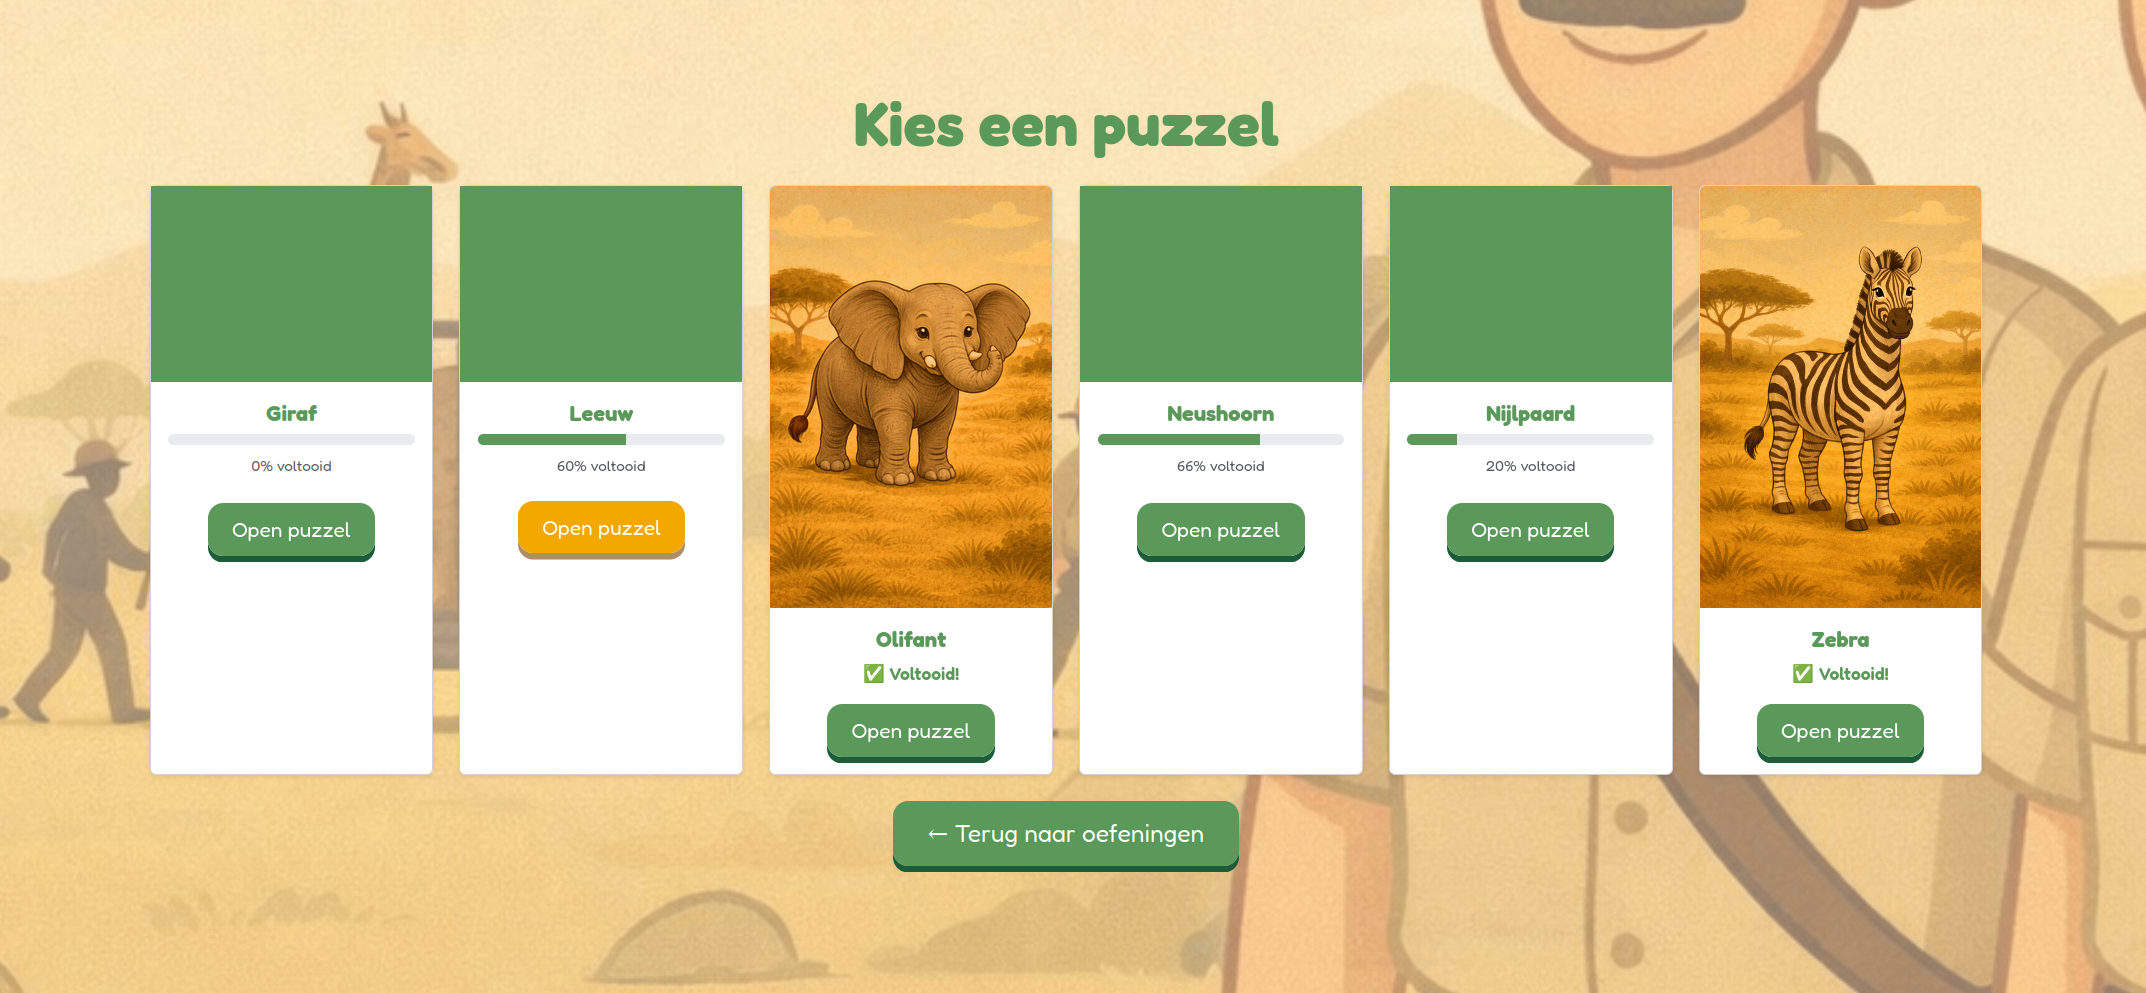
\includegraphics[width=0.85\textwidth]{figures/puzzle-home-new.png}
\caption{The RekenRangers puzzle environment. }
\label{fig:puzzle-home}
\end{figure}

The safari theme is not limited to the reward system. It runs through the entire application: the background illustrations, the button styles, the icons, and the login screen are all designed around the same visual identity. This consistency reinforces the idea that the child is inside a world, not just using a tool. All visual assets, including background scenes and animal images, were created using generative AI and then selected and adapted to fit the visual style of the application.

\subsection{Feedback}
After every exercise, the child receives immediate feedback on their answer. If the answer is correct, the screen shows a short confirmation message. If the answer is wrong, the correct answer is displayed alongside the child's attempt, so that the child can see exactly where they went wrong. The feedback is deliberately kept simple and direct: no elaborate explanations or worked-out solutions, just a clear signal of correctness and, when needed, the right answer. This choice connects back to Section~\ref{sec:exercise-properties}, where the literature on educational feedback suggested that minimal, focused feedback can support children's persistence and strategy use at least as well as more elaborate variants. Extending this with worked-out explanations or hints could still be valuable, particularly for harder operations, and was kept simple here partly because the scope of the supported exercises (single-step addition, subtraction, and multiplication) and the time constraints of the project did not require more.

When the metacognitive self-assessment setting is enabled, a second layer of feedback is added. After each exercise, the child is asked to judge their own answer using a row of four smileys ranging from confident-correct (green) to confident-wrong (red). Once both the answer and the self-assessment are submitted, the feedback screen evaluates both. The self-assessment is considered correct if the child's confidence matched the actual outcome: selecting green or yellow when the answer was right, or orange or red when it was wrong. If the child misjudged their own performance, the feedback tells them so explicitly. Figure~\ref{fig:feedback-screen} shows an example of an exercise that was answered incorrectly but where the child correctly anticipated the mistake.

\begin{figure}
\centering
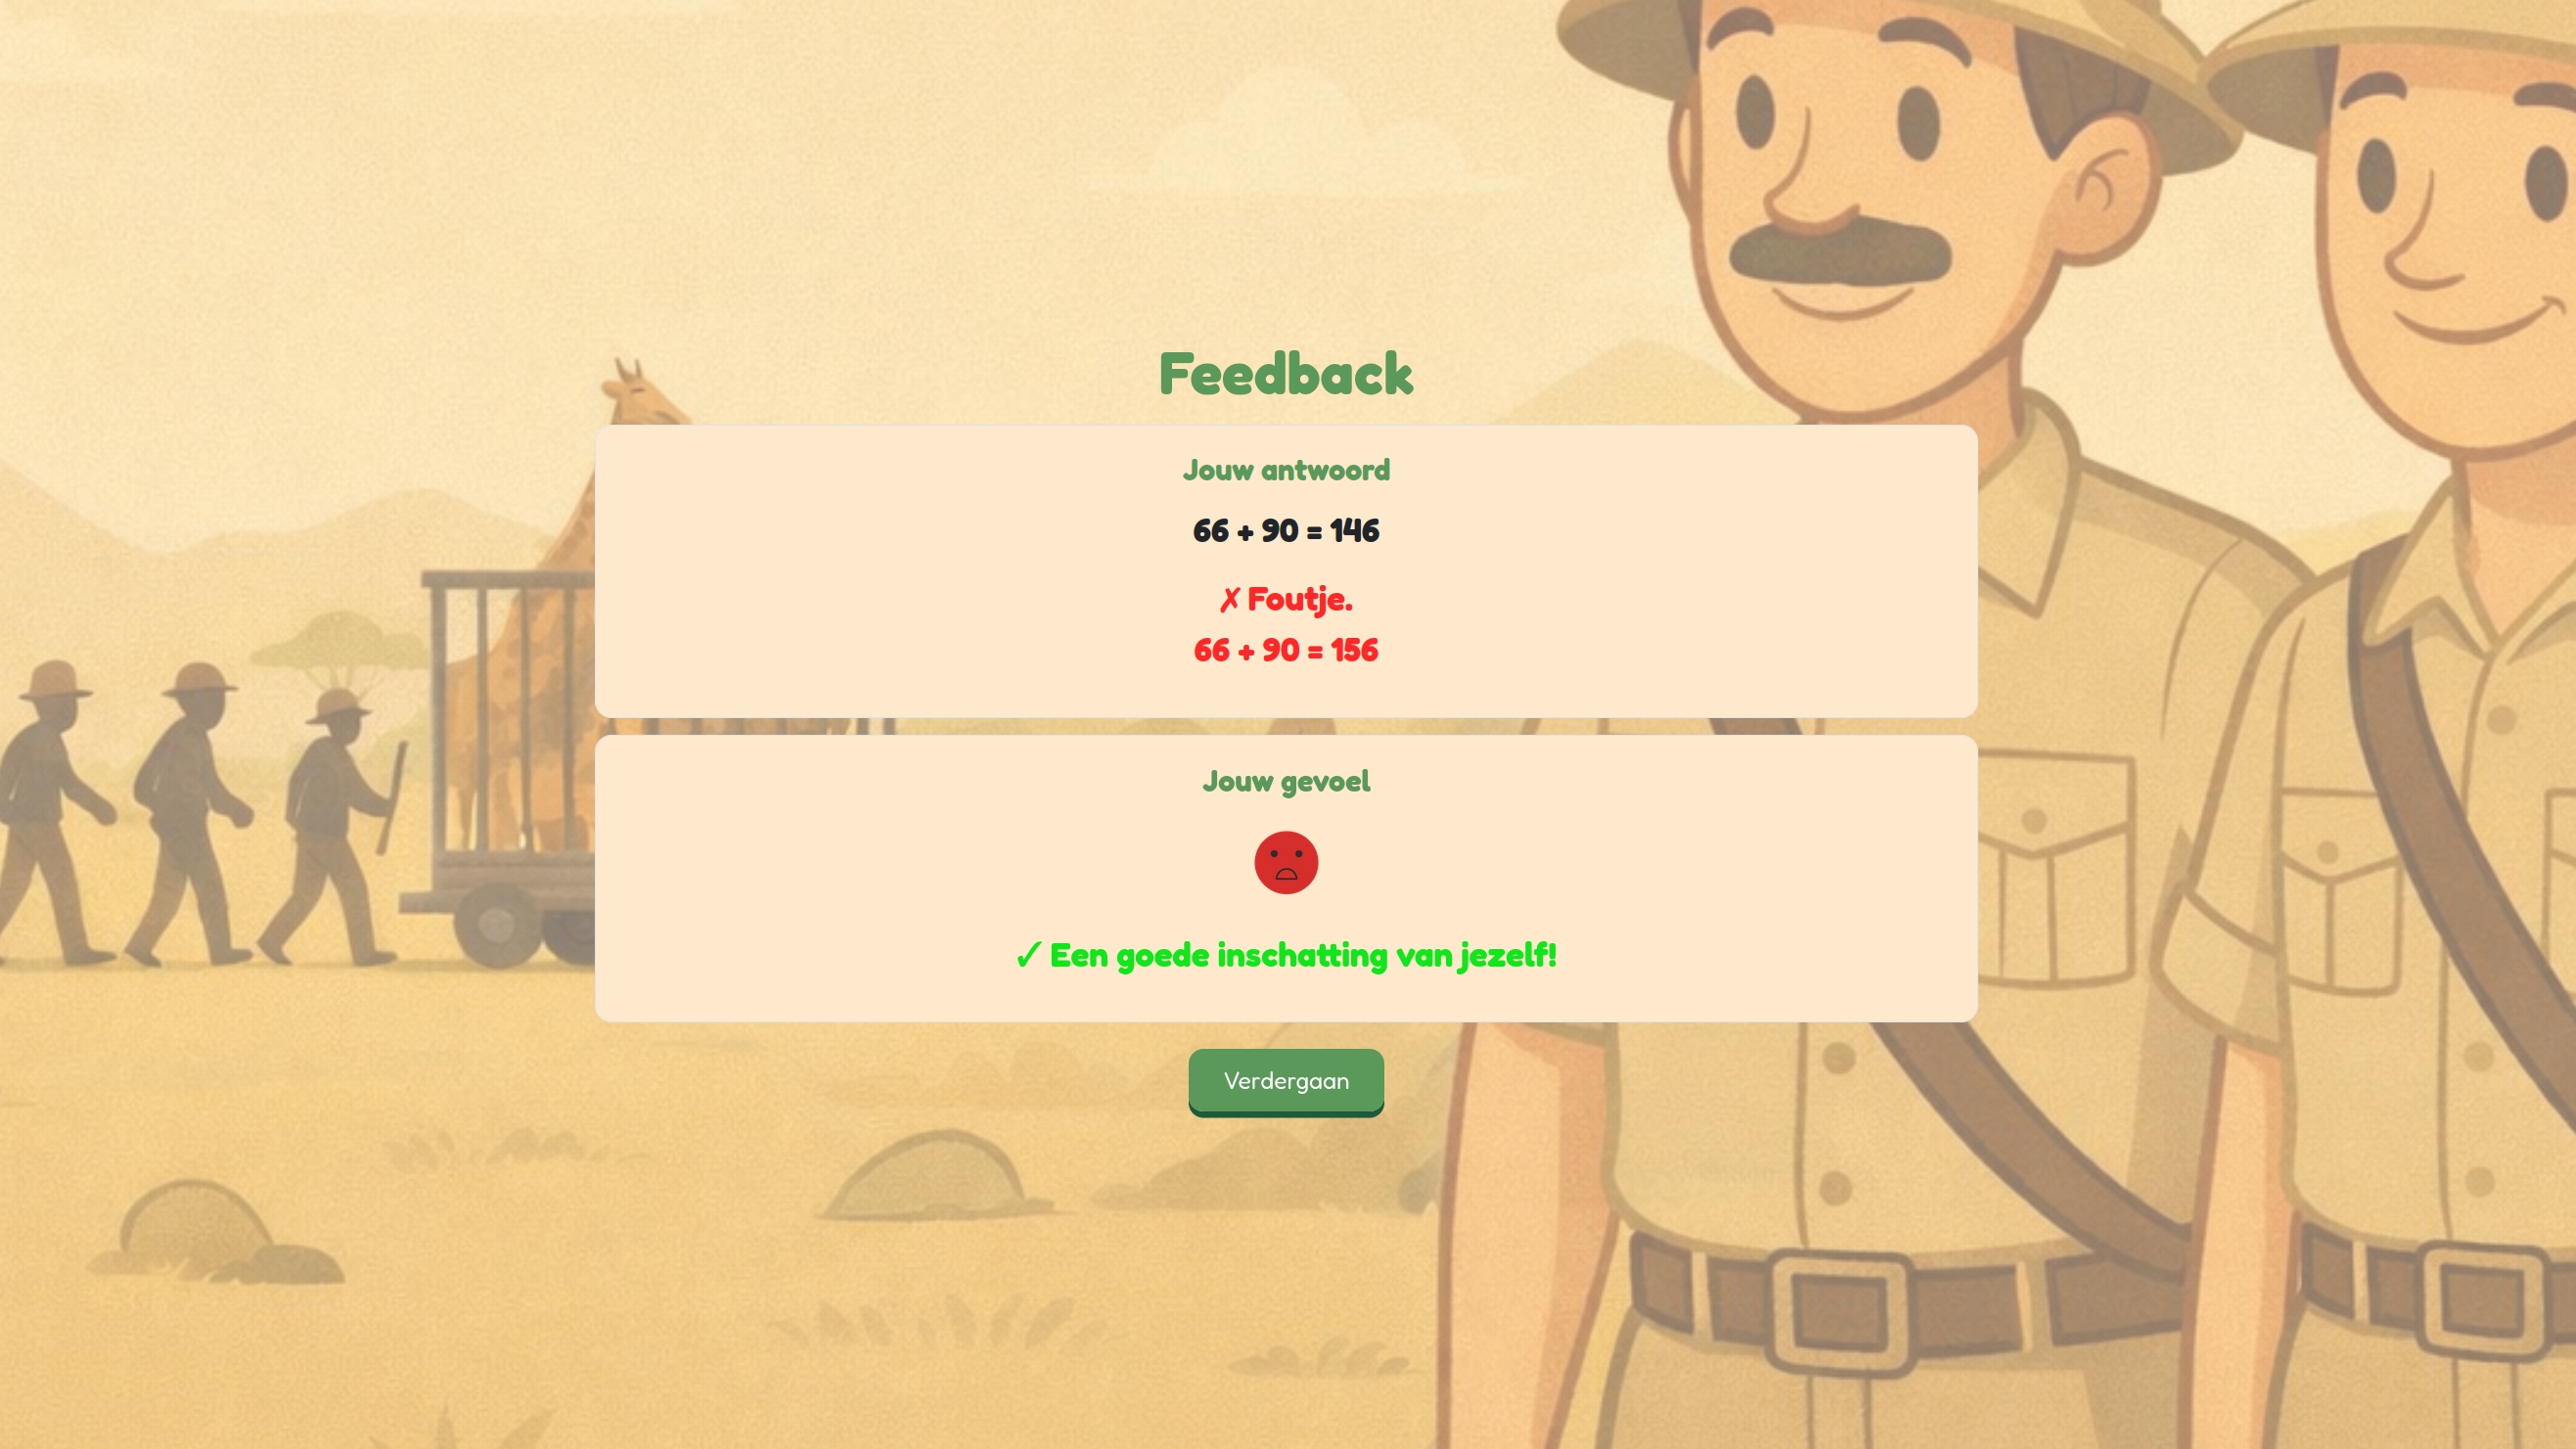
\includegraphics[width=0.85\textwidth]{figures/feedback.png}
\caption{Feedback screen after an incorrectly answered exercise, where the child correctly anticipated the mistake through their self-assessment.}
\label{fig:feedback-screen}
\end{figure}

The confidence judgement paradigm used here mirrors the one in the Bellon et al. study \cite{bellon_more_2019}, and the smileys give it a visual language that is accessible to children as young as seven.

\subsection{Personalisation}
Personalisation is the property where RekenRangers has the most room for growth. The original intention was to integrate an avatar system into the safari theme, where each child would have their own ranger character that could be customised with outfits and accessories purchased with earned coins. Due to time constraints and the need to prioritise the research-critical features, this was not implemented in the current version of the platform.

What RekenRangers does offer is a form of functional personalisation. When enabled by the teacher or researcher, children can choose for themselves which operation they want to practise, what difficulty level they prefer, and whether they want to see a timer. These choices give children a degree of control over their own learning experience, which as discussed in Section \ref{sec:exercise-properties} can support metacognitive awareness and a sense of ownership. Additionally, each child works with their own account, and their coin balance and puzzle progress are personal to them. A child who has saved up coins and completed three animal puzzles sees a different puzzle screen than a classmate who just started. This creates some sense of individual identity within the platform, even without a visual avatar.

The foundation for deeper personalisation is in place. The account system, the coin economy, and the safari theme all lend themselves naturally to extensions such as customisable ranger avatars, personal statistics dashboards, or achievement badges. These are realistic additions for future development and would strengthen a property that is currently functional but not yet fully realised.

\subsection{Accessibility}
RekenRangers is a web application hosted on a KU Leuven server and accessible at \texttt{rekenrangers.cs.kuleuven.be}. It runs in any modern browser without requiring software installation, plugins, or account creation through an external service. This means the tool works on the laptops, tablets, Chromebooks, and even phones that schools and families already have. The only requirements are an internet connection and a browser. There is currently no dedicated mobile app, and the interface is not specifically optimised for smaller screens, but both are realistic extensions for future development.

Access to the platform is managed through a two-step login system designed to be usable by young children without adult help. The child first enters a group code, which identifies their class or research group. They then select their name from a list and enter a personal animal code: a sequence of four animal icons that serves as a child-friendly alternative to a traditional password. Figure~\ref{fig:accessibility} illustrates both the login screen and the printable cards.

\begin{figure}
    \centering
    \begin{subfigure}[t]{\textwidth}
        \centering
        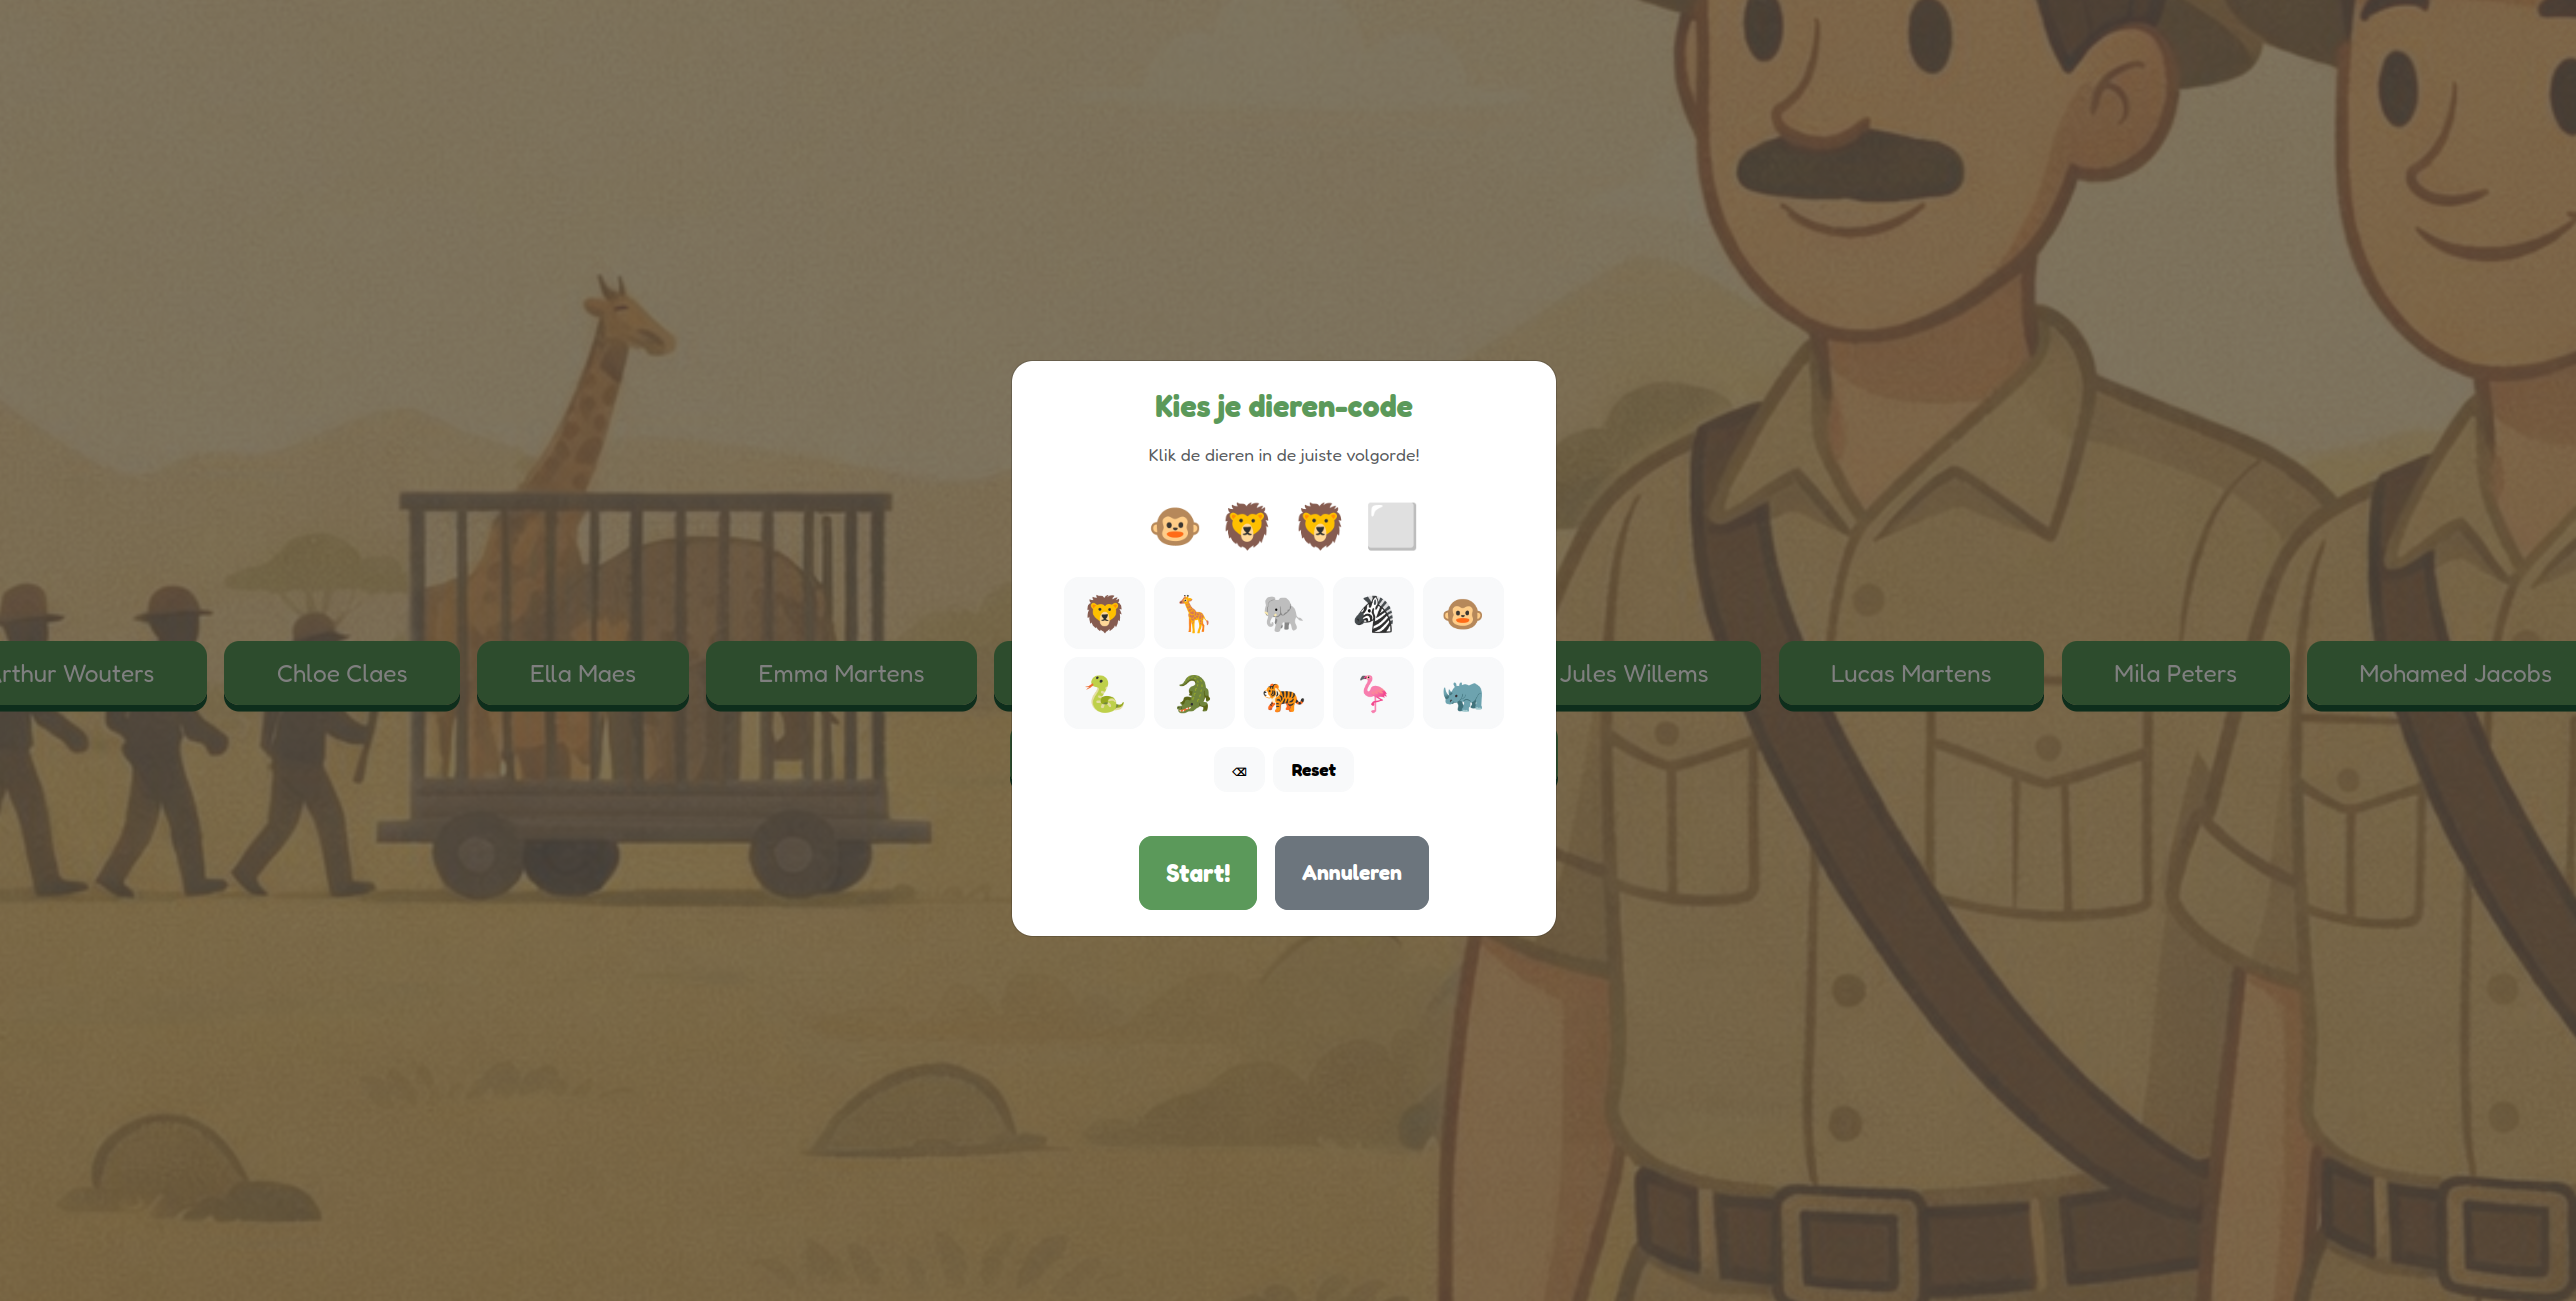
\includegraphics[width=0.8\textwidth]{figures/animal-login.png}
        \caption{The student login screen. After selecting their name, the child enters their personal animal code by clicking four animal icons in the correct order.}
        \label{fig:animal-login}
    \end{subfigure}
    \hfill
    \begin{subfigure}[t]{\textwidth}
         \vspace{0.5cm} 
        \centering
        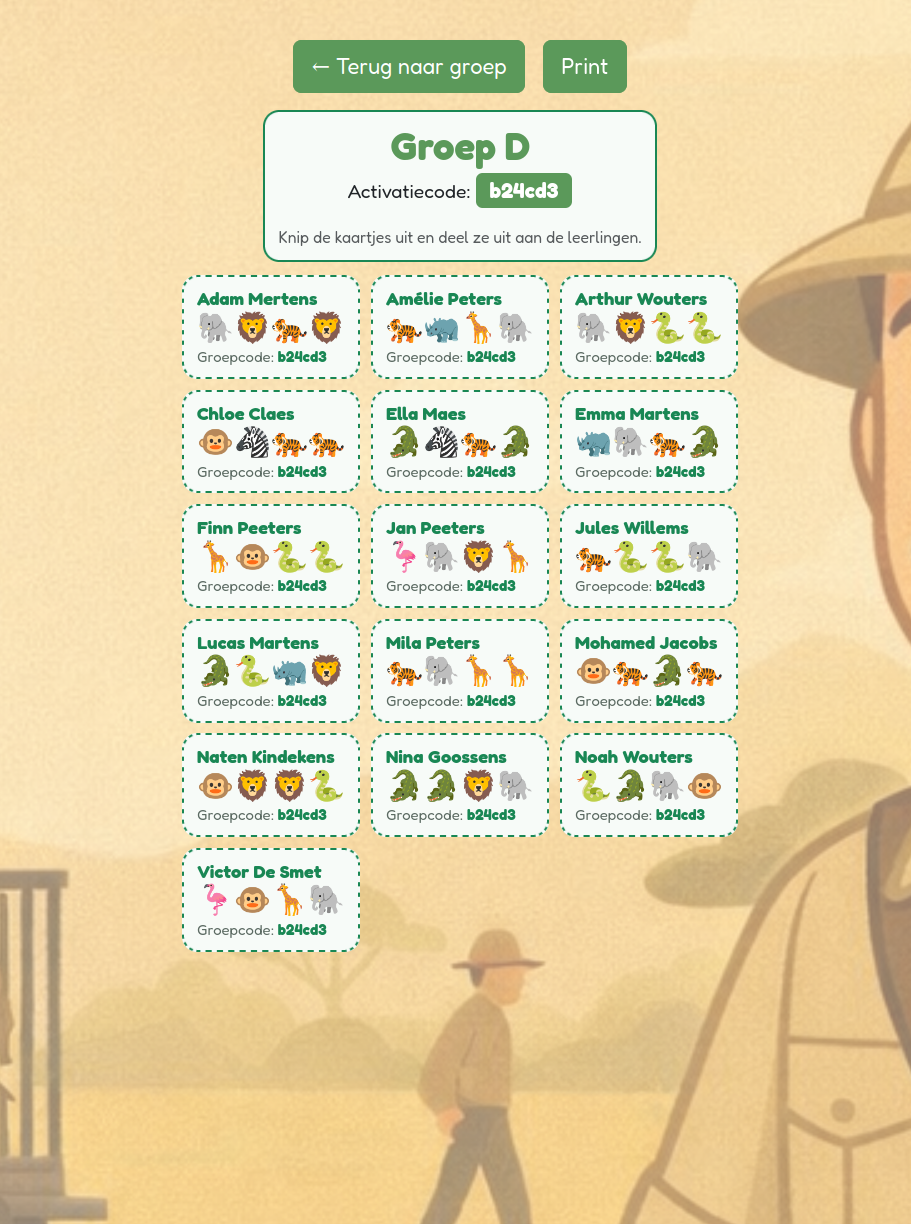
\includegraphics[width=0.4\textwidth]{figures/login-cards.png}
        \caption{Printable login cards generated through the teacher dashboard. Each card shows the child's name, group code, and personal animal code, and can be taken home for use outside the classroom.}
        \label{fig:login-cards}
    \end{subfigure}
    \caption{The RekenRangers login system. Children access the platform using a group code and a personal animal code, both provided through printable cards distributed by the teacher or researcher.}
    \label{fig:accessibility}
\end{figure}

Teachers and researchers generate these cards through the group management screen in the teacher dashboard. The cards can be printed and handed out in class, and since they contain everything a child needs to log in, they also enable use at home. This low-threshold approach to access means that RekenRangers can serve as both a classroom tool and a home practice tool without any additional setup.

\subsection{User friendliness}
The final exercise-tool property is user friendliness, and for RekenRangers this is less a single feature than a principle that runs through every screen of the application. The target audience is children between seven and eleven years old, and every interface element was designed with that in mind. Buttons are large and clearly labelled, navigation follows a simple top-to-bottom flow, and the visual language uses colours, icons, and illustrations rather than relying on text. All text that does appear is written in simple, child-appropriate Dutch.

To help children get started without needing an adult to explain the tool, RekenRangers includes an interactive demo mode. The demo walks the child through the full exercise flow step by step: how to read and answer an exercise, how to submit their answer, how the coin reward works, and how to navigate to the puzzle screen. When the metacognitive self-assessment setting is enabled, a separate version of the demo is available that also explains the smiley-based confidence judgement and what the feedback on it means. The demo can be replayed at any time, so a child who is unsure about something mid-session can revisit the explanation without having to ask for help.

One specific design decision worth mentioning is that the entire child-facing interface can be operated using only the keyboard. Answers are typed in directly, smileys are selected with the f,g,h,j keys, and puzzle pieces are bought with the spacebar. This was a deliberate choice. In pilot sessions, we observed that mouse and trackpad interactions introduced variability in response times that had nothing to do with arithmetic ability. By making the keyboard the primary input method, the tool removes a source of noise from the data, which matters both for the child's experience and for the quality of the research data collected.

The goal behind all of these choices is the same one that Section \ref{sec:exercise-properties} identified through cognitive load theory \cite{sweller1988cognitive}: the interface should be invisible. Every moment a child spends figuring out where to click or what a button means is a moment they are not spending on arithmetic. A well-designed exercise tool is one where the child forgets they are using a tool at all.
% !TeX root = ../thesis.tex
\chapter{Experimental Setup}

\section{How the Bellon et al. study was configured in RekenRangers}

\section{Participants and sessions}

\section{The questionnaire}
\label{sec:questionnaire}
After the final session, each participating child filled in a short paper-based questionnaire about their experience with RekenRangers. The goal was to collect structured feedback on four aspects of the tool: whether children found it motivating, whether they could use it without difficulty, whether it kept them engaged, and whether the feedback and difficulty felt appropriate.\\ \\
Designing a questionnaire for children between eight and eleven years old imposes specific constraints. Questions must be short, concrete, and free of abstract or double-barrelled formulations. Open-ended questions are impractical when the goal is comparable, structured data across a group. And the response scale must be simple enough that a child can use it without hesitation. Research on surveying children confirms that these constraints are not just practical preferences but methodological necessities: younger respondents are more sensitive to question complexity, and poorly formulated items produce unreliable data \cite{borgers2000children}.\\ \\
The questionnaire uses a 4-point Likert scale, where one star means "strongly disagree" and four stars mean "strongly agree." A 4-point scale was chosen to discourage neutral midpoint responses and encourage clearer preference indications.. The stars are presented visually on the paper form, making the scale intuitive without requiring explanation beyond a brief legend at the top of the page.\\ \\
The items are organised around four themes. Motivation is assessed through items about whether the child enjoyed using the tool and whether they would want to use it again. User friendliness is assessed through items about whether the child understood what to do and whether they needed help. Engagement is captured by asking whether RekenRangers made practising arithmetic more interesting. Feedback and difficulty alignment are assessed by asking whether the child understood the correctness feedback and whether the exercises matched their ability level.\\ \\
Two of the seven items are deliberately phrased in the negative direction: "I would not want to use RekenRangers again" and "The exercises did not match my ability well." This is a standard technique in questionnaire design to detect acquiescence bias, the tendency of respondents to agree with every statement regardless of its content. If a child gives four stars to both "I enjoyed using RekenRangers" and "I would not want to use RekenRangers again," this signals inattentive or biased responding and allows the researcher to flag that response for closer inspection.\\ \\
The items were not taken from an existing validated instrument, but are informed by established research traditions. The motivation items align with the principles measured by the Intrinsic Motivation Inventory \cite{ryan1982control}, and the user ffriendliness items reflect the core concerns of the System Usability Scale \cite{brooke1996sus}, both simplified substantially to be appropriate for young children. The full questionnaire is included in Appendix~\ref{app:questionnaire}.\\ \\
% !TeX root = ../thesis.tex
\chapter{Results}

\section{Data quality and completeness}

\section{The adaptive system in practice}
The adaptive difficulty system described in Section~\ref{sec:adaptivity} was used in two of the four experimental conditions (C and D). The non-adaptive conditions (A and B) presented exercises drawn from a balanced mix of all three difficulty levels in a semi-random order. This section examines how the adaptive system behaved in practice using both quantitative data and qualitative observations.\\ \\

\subsection{Elo trajectories}
Figure~\ref{fig:elo-trajectories} shows the Elo trajectories of five randomly selected participants from the adaptive conditions over the course of their 216 exercises. All five children started at the initial rating of 450, but their paths diverge quickly. The strongest participant (blue) climbed rapidly and reached the ceiling of 1000 within the first 50 exercises, remaining there for the rest of the study. Two others (green and orange) followed a slower upward trend, stabilising in the 800--950 range by the end of the training period. The remaining two (red and purple) settled in the 600--800 range, with visible fluctuations that reflect the system adjusting to their performance on individual exercises.\\ \\
Two things are worth noting. First, the trajectories are not smooth curves but jagged paths with frequent ups and downs. This is expected behaviour: the Elo system responds to every exercise, and a single mistake produces an immediate dip. The overall trend, however, is clearly readable in each case. Second, the five trajectories end up at genuinely different levels, which means the system is capturing real individual differences in ability rather than pushing everyone toward the same point.\\ \\
\begin{figure}[ht]
\centering
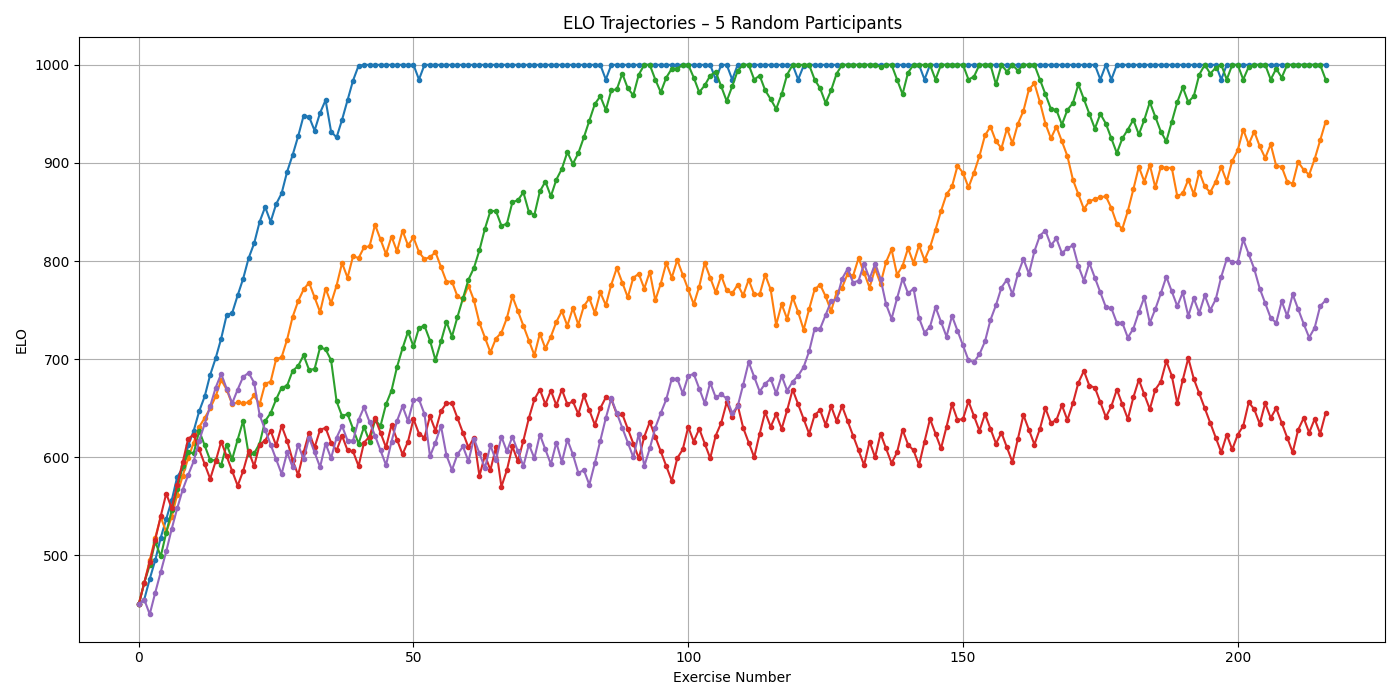
\includegraphics[width=\textwidth]{figures/sample_trajectories.png}
\caption{Elo rating trajectories of five randomly selected participants from the adaptive conditions. All participants started at a rating of 450. The trajectories illustrate how the system differentiates between children of different ability levels over the course of 216 exercises.}
\label{fig:elo-trajectories}
\end{figure}

\subsection{Final Elo distribution}
Figure~\ref{fig:elo-distribution} shows the distribution of final Elo scores across all participants in the adaptive conditions. The distribution spans from approximately 500 to 1000, with a main cluster around 600--700 and a second, distinct peak at the maximum rating of 1000. The main cluster sits in difficulty zone 4 (600--800), meaning these children were predominantly receiving difficult and medium exercises by the end of the training. The peak at 1000 represents children who reached the ceiling and stayed there. For these children, the exercise pool could no longer offer sufficient challenge, as all exercises were already drawn from the highest difficulty level.\\ \\
\begin{figure}[ht]
\centering
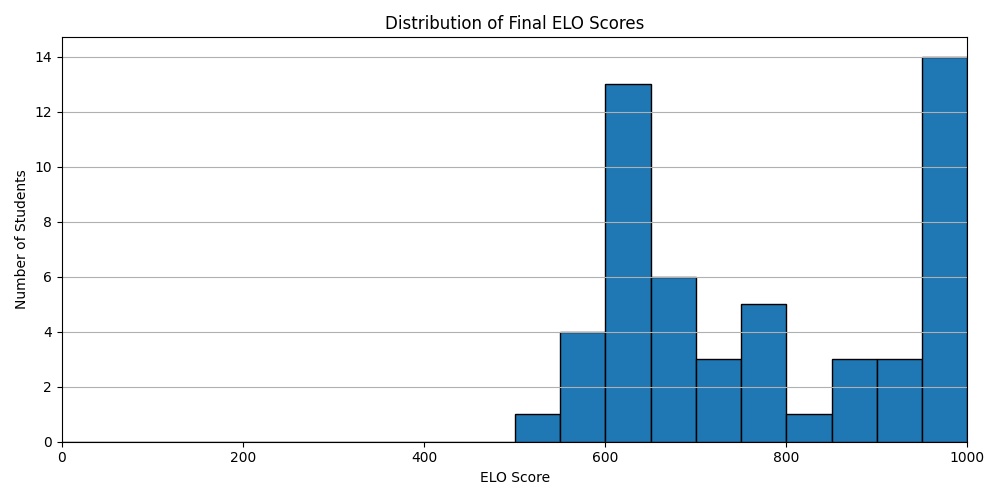
\includegraphics[width=0.8\textwidth]{figures/elo_distribution_histogram.png}
\caption{Distribution of final Elo scores across participants in the adaptive conditions. The main cluster around 600--700 corresponds to difficulty zone 4. The peak at 1000 represents children who reached the rating ceiling.}
\label{fig:elo-distribution}
\end{figure}

\subsection{Accuracy rates}
Figure~\ref{fig:accuracy-distribution} compares the distribution of per-student accuracy rates between the adaptive and non-adaptive conditions. The non-adaptive group achieved a mean accuracy of 76\% (\(\sigma = 0.16\)), which sits close to the 75\% target. The adaptive group achieved a lower mean accuracy of 68\% (\(\sigma = 0.14\)). The difference is expected: children in the adaptive conditions faced a higher average exercise difficulty (mean difficulty level of 2.54, compared to 2.00 in the non-adaptive conditions, where difficulty levels were balanced by design). The adaptive system pushed stronger children toward harder exercises, which increased the error rate.
However, the adaptive system did not converge on the intended 75\% accuracy target. The mean accuracy of 68\% indicates that the current parameter settings produce a difficulty level that is somewhat too challenging for the average participant. The most likely explanation is that the \(K\) parameter or the scoring function needs further tuning to achieve a closer match with the target. This is discussed further in Section \myworries{IN WHICH SETION IN DISCUSSIOn}.
\begin{figure}[ht]
\centering
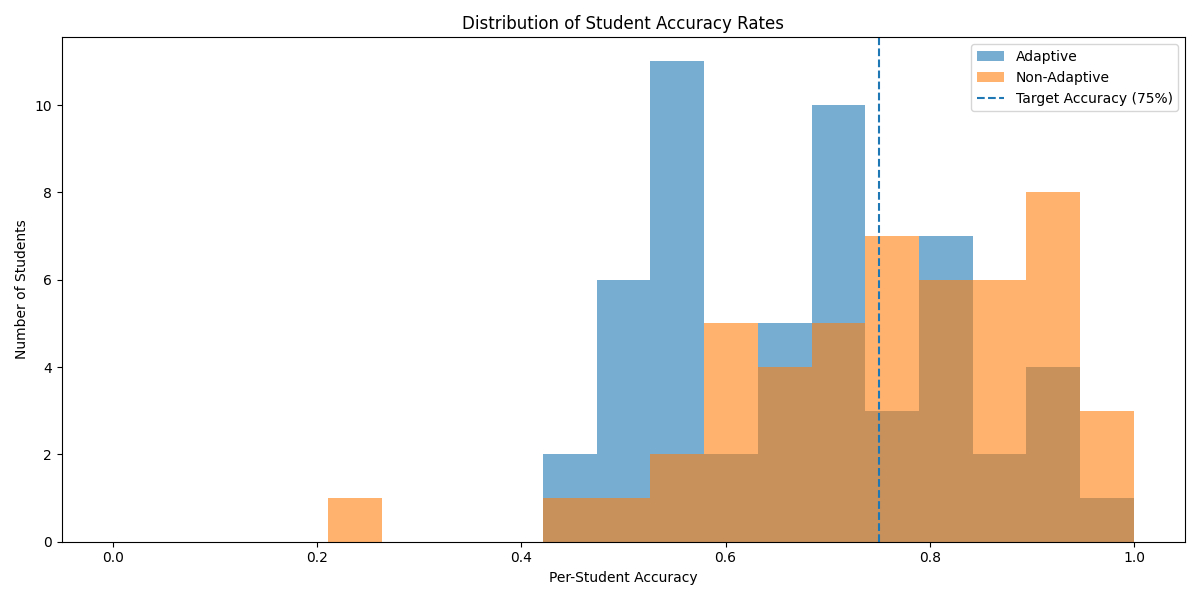
\includegraphics[width=\textwidth]{figures/accuracy_distribution_histogram.png}
\caption{Distribution of per-student accuracy rates for the adaptive and non-adaptive conditions. The dashed line marks the 75\% target accuracy. The adaptive group (mean 68\%) falls below the target, while the non-adaptive group (mean 77\%) lands close to it.}
\label{fig:accuracy-distribution}
\end{figure}

\subsection{Response times}
Figure~\ref{fig:response-time-distribution} shows the distribution of mean response times per student for both groups. The non-adaptive group shows a wide, relatively uniform spread across response times, ranging from around 6 to 14 seconds. This is consistent with the fact that these children received exercises from all three difficulty levels regardless of their ability: strong children solved easy exercises quickly while weaker children spent longer on the harder ones, producing a flat distribution. The adaptive group shows a different pattern, with a concentration toward longer response times (12--14 seconds). This is consistent with how the scoring function works: the system's equilibrium point occurs when a child answers correctly at approximately the time limit, which means the adaptive algorithm naturally pushes children toward exercises where they need close to the full time available.\\ \\
\begin{figure}[ht]
\centering
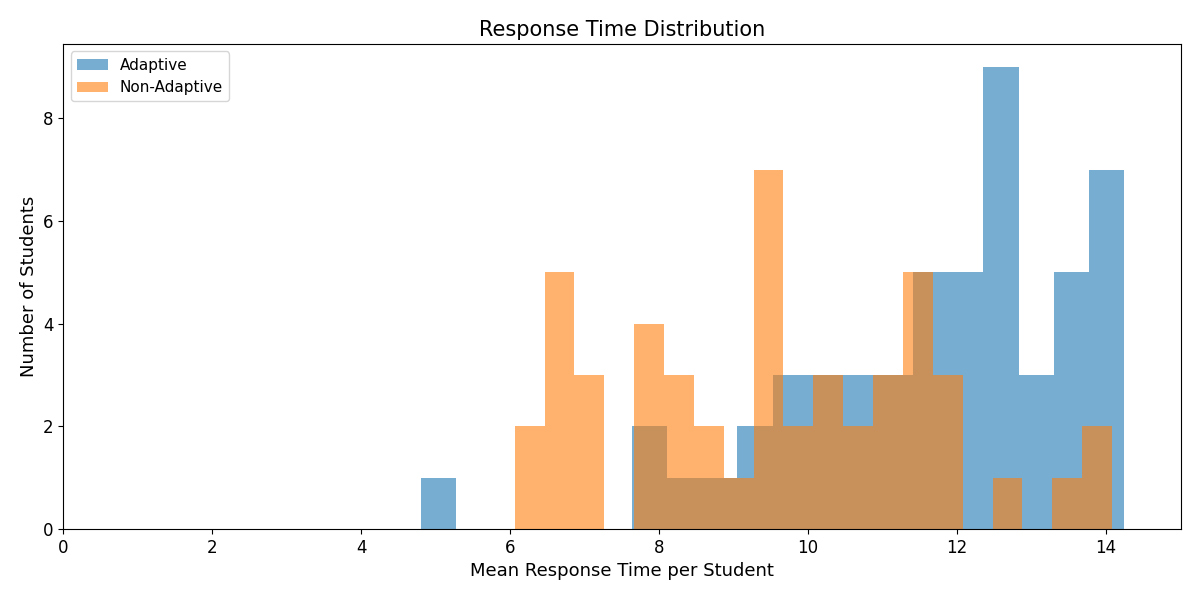
\includegraphics[width=\textwidth]{figures/response_time_distribution.png}
\caption{Distribution of mean response times per student for the adaptive and non-adaptive conditions. The adaptive group clusters toward longer response times, consistent with the scoring function pushing toward the time limit as an equilibrium point.}
\label{fig:response-time-distribution}
\end{figure}

\subsection{Qualitative observations}
The quantitative patterns are supported by observations made during the classroom sessions. In her feedback report, Eline T'joen noted that children in the non-adaptive conditions appeared to lose focus more quickly during exercises, while children in the adaptive conditions remained more consistently engaged. She also observed that the non-adaptive group showed visible signs of frustration or boredom more frequently, which aligns with the theoretical expectation from Section 3.1: when exercises do not match a child's level, the result is either anxiety (too hard) or disengagement (too easy). The adaptive system, despite not hitting its 75\% accuracy target precisely, appears to have produced a more engaging experience by keeping the challenge level closer to each child's ability.

\section{Engagement: coins and puzzles}
One of the central claims of this thesis is that gamification elements help keep children engaged across multiple sessions. The coin and puzzle system in RekenRangers provides a direct way to test this claim with behavioural data rather than self-report alone: if children actively spend their coins on puzzles, they are engaging with the gamification system, and if they complete puzzles, they are treating the animal rescue mission as a genuine subgoal.\\ \\
Table~\ref{tab:coin-summary} summarises the coin and puzzle data across all four conditions. The results are striking. Across the full sample of 107 participants, children spent on average 98.5\% of their earned coins on puzzle pieces. Out of 107 children, nobody spent less then 85\% of their coins. This pattern is consistent across all four conditions, regardless of whether the condition included metacognitive prompts or adaptive difficulty.\\ \\
\begin{table}[ht]
\centering
\small
\setlength{\tabcolsep}{6pt}

\begin{tabular}{@{}lcccccc@{}}
\toprule

Condition & \(n\) & Mean earned & Mean spent & Mean \% spent & Mean puzzles completed \\
\midrule
A & 27 & 671.0 & 659.8 & 98.3 & 2.5 \\
B & 27 & 685.2 & 673.7 & 98.2 & 2.6 \\
C & 27 & 610.4 & 601.9 & 98.6 & 2.0 \\
D & 26 & 620.7 & 613.5 & 98.8 & 2.0 \\
\bottomrule
\end{tabular}

\caption{Average coin earning, spending, and puzzle completion across the four experimental conditions. Children were free to spend or save their coins; no instructions or incentives to buy puzzle pieces were given beyond the narrative framing of the safari story.}
\label{tab:coin-summary}
\end{table}

\noindent It is worth emphasising that children were never instructed to spend their coins. The puzzle shop was available at the end of each training day, and children were told they could buy puzzle pieces if they wanted to, but there was no check or reward for doing so. The near-universal spending behaviour therefore reflects genuine voluntary engagement with the gamification system. The small number of unspent coins per child (on average between 0 and 25 coins depending on the condition) is largely explained by the fact that remaining coins were insufficient to purchase another puzzle piece at the prices available.\\ \\
The puzzle completion data adds a second layer to this picture. Across all conditions, 99\% of children completed at least one puzzle, and 47\% completed three or more over the four training days. The coin system was deliberately designed so that completing all six puzzles within 216 exercises was impossible, ensuring that there was always a next goal to work toward. Interestingly, the data also reveals different purchasing strategies: some children prioritised the cheaper puzzles to complete as many animals as possible, while others saved for more expensive puzzles and ended up with fewer completed puzzles despite having earned a similar number of coins. This variation in strategy suggests that children were not mindlessly clicking through the puzzle shop but were making deliberate choices about how to spend their resources.\\ \\
The difference in mean coins earned between the non-adaptive conditions (A and B, around 680 coins) and the adaptive conditions (C and D, around 615 coins) is expected: the adaptive system presents harder exercises to stronger children, which increases response times and reduces the coin bonus for speed. This does not appear to have affected engagement, as the spending percentages in all four conditions were in fact highly similar.\\ \\

\section{Questionnaire results}

\section{Researcher feedback}

% !TeX root = ../thesis.tex
\chapter{Discussion}
\label{chp:discussion}

\section{Interpretation of results}
The central question behind this thesis is whether a single tool can bridge the gap between classroom exercise tools and controlled research software. The results from the classroom deployment with 107 participants across four conditions and four training days provide a first answer.

\subsection*{Did the tool work as a research instrument?}
On the research side, RekenRangers demonstrated that it can support a real experiment from start to finish. Two researchers with no programming background configured a 2$\times$2 factorial study, deployed it across seven schools, ran it over multiple days, monitored participant progress through the dashboard, and exported structured data ready for analysis. There were problems along the way (the duplicate submission bug, a server downtime incident, a demo that was too long) but none of these resulted in permanent data loss or forced the study to be abandoned. The final results of the study itself are not yet available, as Eline T'joen and Kiara Willems will complete their master's thesis in the next academic year. But the fact that the tool carried a study of this scale and complexity is itself a meaningful result. It shows that the gap identified in Chapters \ref{chp:background} and \ref{chp:exercise-tools} is not just a theoretical concern but one that can be addressed in practice.

\subsection*{Did the engagement system deliver?}
The engagement data tells a clearer story. Children spent 98.5\% of their earned coins on puzzle pieces, and 99\% completed at least one puzzle, all without any instruction or incentive to do so. The variation in purchasing strategies (some children going for cheap puzzles to rescue as many animals as possible, others saving for expensive ones) suggests that children were making deliberate choices rather than clicking through the shop mechanically. From the qualitative feedback, Eline reported that children were visibly enthusiastic about the puzzles and the safari theme. What the data cannot show is whether this engagement translated into better arithmetic performance or more sustained accuracy over the four training days. Demonstrating a causal link between gamification and learning outcomes would require a dedicated study with engagement as the independent variable, which was outside the scope of this thesis.

\subsection*{Did the adaptivity system perform as designed?}
The adaptive difficulty system produced mixed results. On the positive side, it clearly differentiated between children of different ability levels: final Elo scores ranged from 500 to 1000, and the trajectory data shows the system responding to each child individually. Children in the adaptive conditions received exercises closer to their own level (mean difficulty of 2.54 compared to the fixed 2.00 in non-adaptive conditions), and the response time data confirms that the scoring function pushed children toward exercises where they needed close to the full time available. These are signs that the system is doing what it was designed to do: keeping children in a zone where the exercises are challenging but not impossible. On the other hand, the system did not converge on its 75\% accuracy target. The mean accuracy of 68\% in the adaptive conditions indicates that the current calibration is too aggressive. The most likely causes are the fixed expected score of 0.75 and the scoring function \ref{for:scoring-function}, both of which were set based on limited pilot data. A more refined approach would be to assign an Elo rating to each individual exercise rather than working with fixed difficulty categories, following the item-level model used in Rekentuin \cite{klinkenberg2011computer}. This would allow the system to learn which specific exercises are hard and which are easy, rather than relying on a predefined classification. The ceiling effect, with 14 children reaching the maximum Elo of 1000, points in a similar direction: the current exercise pool does not extend far enough at the top end, and either harder exercises or a wider rating scale would be needed to keep the system informative for the strongest children. These are calibration and content problems rather than architectural ones. The adaptive framework itself is sound and can be improved incrementally.\\ \\
The response time difference between the adaptive and non-adaptive groups is worth a brief note. The adaptive group clustered toward longer response times, while the non-adaptive group was spread more uniformly. This is a direct consequence of the scoring function, whose equilibrium point sits at the time limit. The pattern confirms that the system behaves as designed, but it also raises the question of whether pushing children to work at the edge of their time limit is pedagogically desirable. A scoring function with a more generous equilibrium might produce a more comfortable experience without sacrificing the adaptive mechanism.



\section{Limitations}
\label{sec:limitations}

\section{Collaborating across disciplines: reflections for a computer scientist}


% !TeX root = ../thesis.tex
\chapter{Conclusion and Future Work}
\label{chp:conclusions}

\section{Conclusion}

\section{Future work}
\label{sec:future-work}

\appendix

\chapter{Exercise Specification}
\label{app:exercise-spec}

RekenRangers supports three arithmetic operations: addition, subtraction, and multiplication. For each operation, exercises are classified into three difficulty levels based on properties of the operands and the result. This appendix describes the classification rules for each operation.

\section{Addition}

The difficulty of an addition exercise $a + b = s$ is determined by the magnitude of the operands and whether the addition requires carrying (i.e., whether the sum of the unit digits exceeds or equals 10).

\begin{table}[ht]
\centering
\begin{tabular}{cp{10cm}}
\toprule
Level & Criteria \\
\midrule
1 (easy) & The sum is less than 10. Both operands are single-digit numbers and the result stays within the single digits. \\
2 (medium) & The sum is 10 or greater, but no carrying is required, except for two single digits. This includes cases where both operands are single-digit and the sum just crosses 10, as well as cases involving two-digit operands where the unit digits sum to less than 10. \\
3 (difficult) & Both operands are two-digit numbers and carrying is required: the sum of the unit digits is 10 or greater. \\
\bottomrule
\end{tabular}
\caption{Difficulty classification for addition exercises.}
\label{tab:diff-addition}
\end{table}

\section{Subtraction}

The difficulty of a subtraction exercise $a - b$ (where $a \geq b$) depends on the magnitude of the operands and whether borrowing is required (i.e., whether the unit digit of $a$ is smaller than the unit digit of $b$).

\begin{table}[ht]
\centering
\begin{tabular}{cp{10cm}}
\toprule
Level & Criteria \\
\midrule
1 (easy) & Both operands are single-digit numbers and the result is less than 10. \\
2 (medium) & At least one operand is a two-digit number, but no borrowing is required: the unit digit of $a$ is greater than or equal to the unit digit of $b$. \\
3 (difficult) & Both operands are two-digit numbers and borrowing is required: the unit digit of $a$ is smaller than the unit digit of $b$. \\
\bottomrule
\end{tabular}
\caption{Difficulty classification for subtraction exercises.}
\label{tab:diff-subtraction}
\end{table}

\section{Multiplication}

The difficulty of a multiplication exercise $a \times b = p$ is based on the magnitude of the operands and the product.

\begin{table}[ht]
\centering
\begin{tabular}{cp{10cm}}
\toprule
Level & Criteria \\
\midrule
1 (easy) & The product is at most 25. These are small multiplication facts that children typically memorise early. \\
2 (medium) & Both operands are at most 10 (single-digit multiplication tables), but the product exceeds 25. \\
3 (difficult) & Both operands are at most 20, with exactly one operand exceeding 10. These exercises require multiplying a single-digit number by a two-digit number. \\
\bottomrule
\end{tabular}
\caption{Difficulty classification for multiplication exercises.}
\label{tab:diff-multiplication}
\end{table}

\noindent These classification rules are implemented as deterministic functions in the back-end. When the adaptive system selects an exercise, it first determines which difficulty level to draw from (based on the child's current rating and the distribution in Table~\ref{tab:difficulty-zones}), then generates a random exercise that satisfies the corresponding criteria.\\ \\
The difficulty classification described above is based on the categorisation of arithmetic exercises used in the Flemish primary school mathematics curriculum \cite{REF_CURRICULUM}, which distinguishes exercises by operand magnitude and the presence or absence of carrying and borrowing as key indicators of cognitive complexity.

\chapter{Data Fields}
\label{app:data-fields}

Table~\ref{tab:data-fields} lists all fields recorded for each exercise completed in RekenRangers.

\begin{table}[ht]
\centering
\begin{tabular}{lp{9cm}}
\toprule
Field & Description \\
\midrule
user & The student who completed the exercise \\
set\_id & Unique identifier linking all exercises completed in one session \\
operation & The arithmetic operation (addition, subtraction, or multiplication) \\
left\_operand & The first operand of the exercise \\
right\_operand & The second operand of the exercise \\
user\_answer & The answer entered by the child \\
real\_answer & The correct answer \\
is\_correct & Whether the child's answer was correct \\
response\_time & Time taken to answer the exercise (in milliseconds) \\
timestamp & The exact date and time the exercise was completed \\
difficulty & The difficulty level of the exercise (1, 2, or 3) \\
timer\_visible & Whether the timer was visible to the child during the exercise \\
confidence\_judgement & The self-assessment smiley selected by the child (if enabled) \\
confidence\_calibration & Whether the self-assessment matched the actual outcome \\
response\_time\_selfscore & Time taken to select the confidence judgement \\
response\_time\_feedback & Time spent on the feedback screen \\
current\_elo & The child's Elo rating at the time of the exercise \\
delta\_elo & The change in Elo rating produced by this exercise \\
difficulty\_zone & The difficulty zone the child was in (1 through 5) \\
\bottomrule
\end{tabular}
\caption{Complete list of data fields recorded for each exercise in RekenRangers.}
\label{tab:data-fields}
\end{table}
\chapter{Group Settings}
\label{app:group-settings}

Table~\ref{tab:group-settings} lists all configurable settings available in the RekenRangers teacher dashboard for each group.

\begin{table}[ht]
\centering
\begin{tabular}{lp{8.5cm}}
\toprule
Setting & Description \\
\midrule
\multicolumn{2}{l}{\textit{General settings}} \\
\midrule
Timer mode & Whether children can choose to show or hide the timer. \\
Timer visibility & Whether the timer is forced on or off. \\
Available operations & Which operations are available: addition, subtraction, multiplication, or a mix \\
Mix composition & When mix is selected, which operations are included \\
Difficulty mode & Adaptive (Elo-based), fixed by the researcher, or chosen by the child \\
Fixed difficulty level & When fixed, the difficulty level (1, 2, 3, or a mix) \\
Metacognitive prompting & Whether the self-assessment smiley prompt is shown after each exercise \\
\midrule
\multicolumn{2}{l}{\textit{Research settings}} \\
\midrule
Research mode & Disables mouse interaction, hides non-essential buttons, and standardises interface text \\
Demo with metacognition & Whether the interactive demo includes the self-assessment explanation \\
Fixation screen & Whether a fixation cross is displayed before each exercise \\
Prevent identical exercises & Blocks the same exercise from appearing twice in one session \\
Exclude tie problems & Prevents exercises where both operands are equal \\
Prevent repeated results & Blocks exercises with the same outcome from appearing consecutively \\
Commutativity & Treats commuted exercises (e.g., $3 \times 7$ and $7 \times 3$) as identical \\
Operand position balance & Balances whether the larger operand appears on the left or right \\
Excluded values (operand A) & List of values that may not appear as the first operand \\
Excluded values (operand B) & List of values that may not appear as the second operand \\
Excluded values (result) & List of values that may not appear as the answer \\
\bottomrule
\end{tabular}
\caption{Complete list of group settings available in the RekenRangers teacher dashboard.}
\label{tab:group-settings}
\end{table}
\chapter{Teacher and researcher manual}
\label{app:teacher-manual}

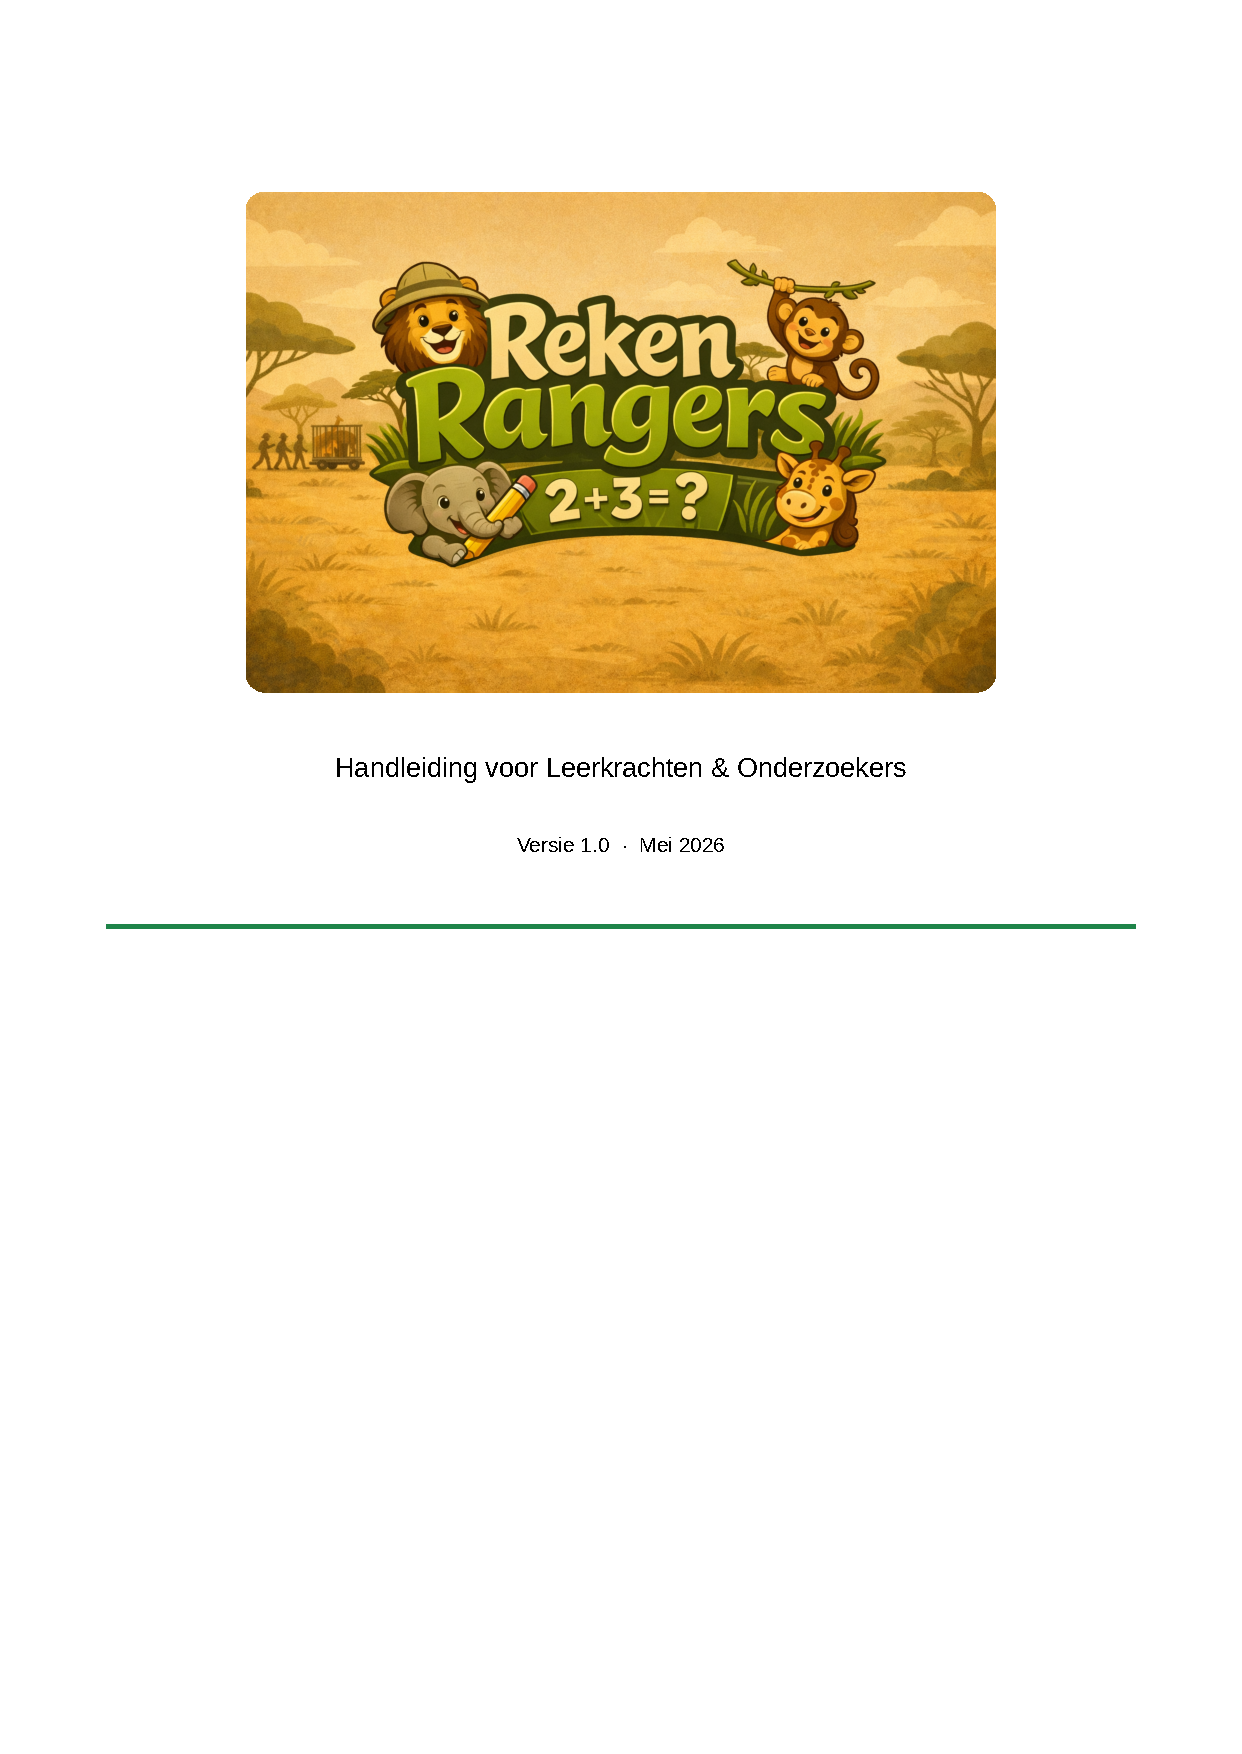
\includepdf[pages=-]{figures/handleiding.pdf}
\chapter{Questionnaire}
\label{app:questionnaire}
% Include the questionnaire PDF
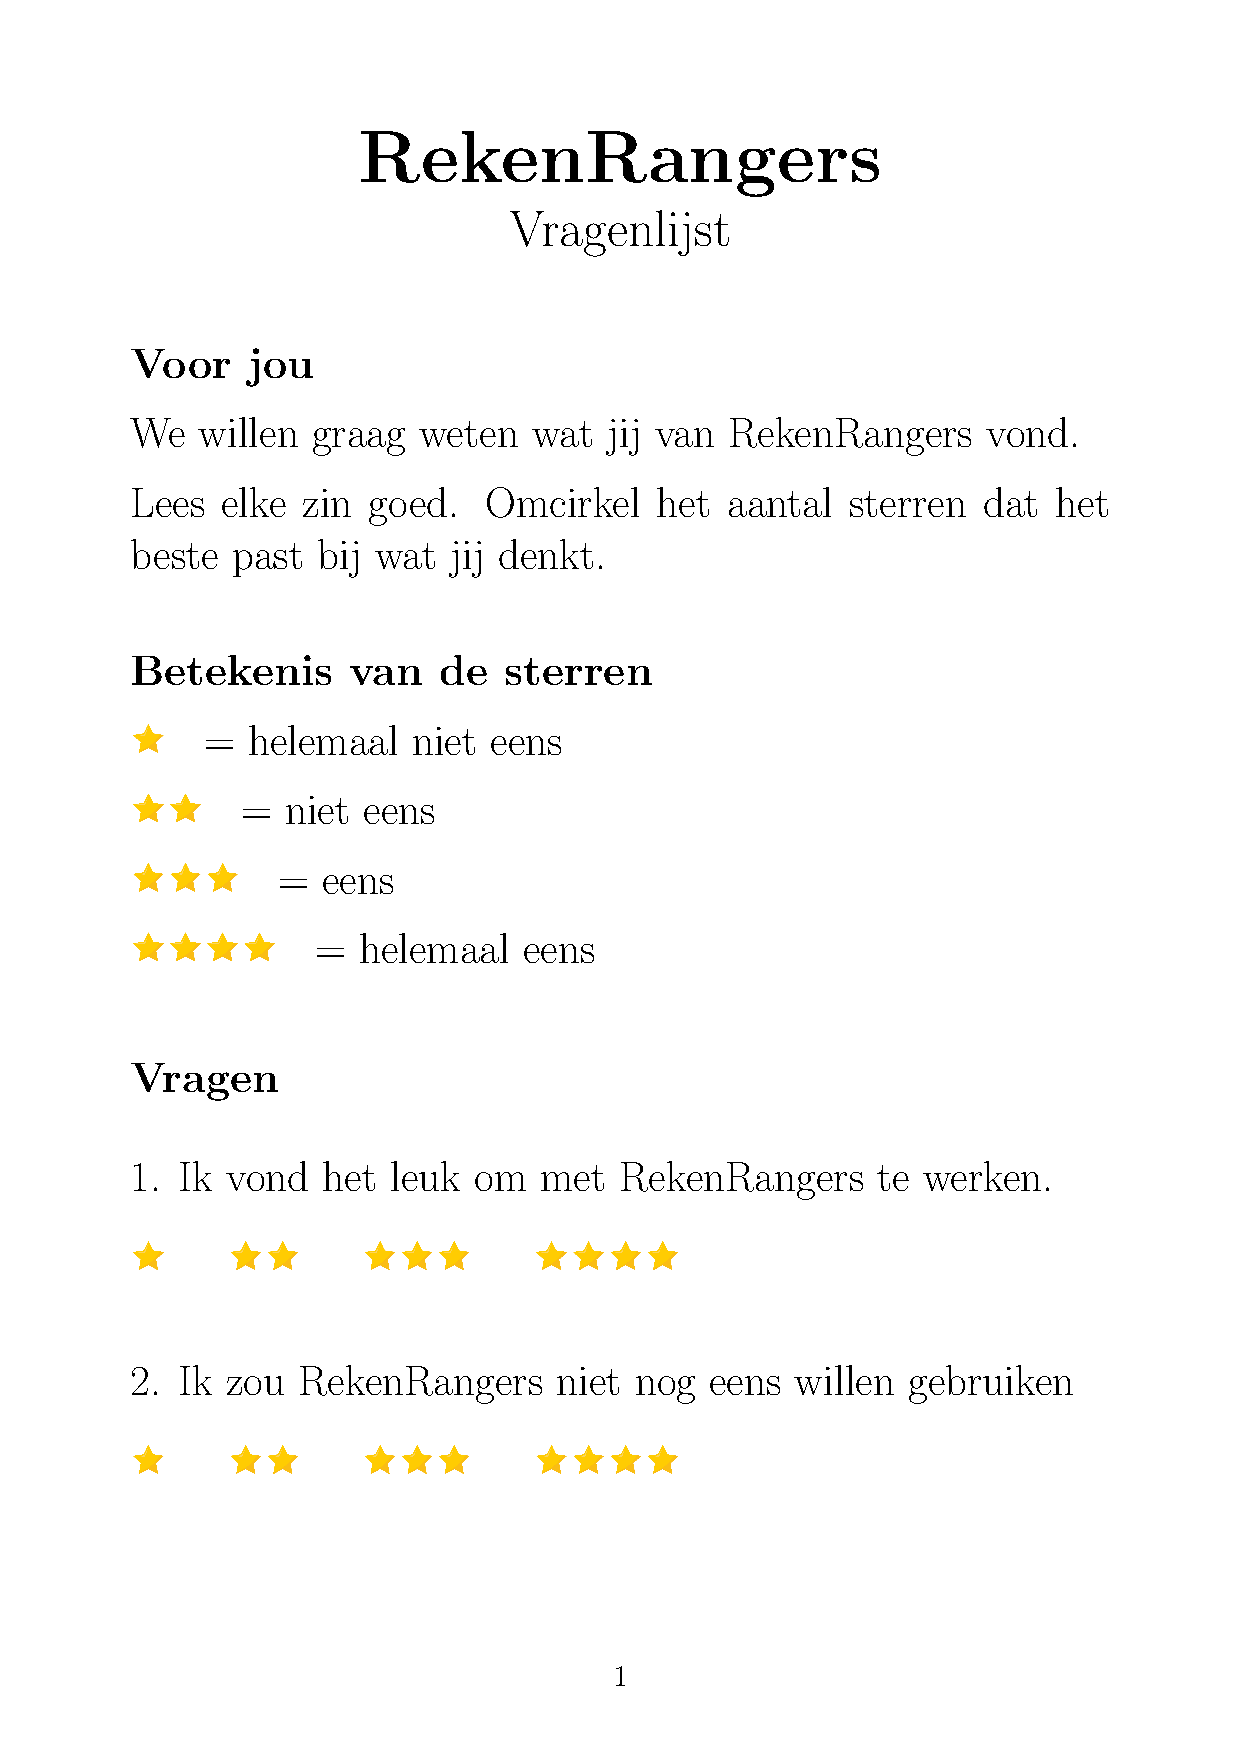
\includepdf[pages=-]{figures/questions_rekenrangers.pdf}

% === Bibliography ===
\backmatter
\bibliographystyle{abbrv}
\bibliography{references}



\end{document}
